%!TeX encoding = UTF-8
%!TEX TS-program = pdflatex
% Author: Phil Steinhorst, p.st@wwu.de
%!TEX root = thesis.tex
% Author: Phil Steinhorst, p.st@wwu.de

% **************************************************
% Document Class Definition
% **************************************************
\documentclass[%
	paper=A4,					% paper size --> A4 is default in Germany
	twoside=true,				% onesite or twoside printing
	openright,					% doublepage cleaning ends up right side
	parskip=full,				% spacing value / method for paragraphs
	chapterprefix=true,			% prefix for chapter marks
	11pt,						% font size
	headings=normal,			% size of headings
	bibliography=totoc,			% include bib in toc
	listof=totoc,				% include listof entries in toc
	titlepage=on,				% own page for each title page
	captions=tableabove,		% display table captions above the float env
	draft=false,				% value for draft version
]{scrreprt}%

% **************************************************
% Debug LaTeX Information
% **************************************************
%\listfiles

% **************************************************
% Information and Commands for Reuse
% **************************************************
\newcommand{\thesisTitle}{Titel der Masterarbeit}
\newcommand{\thesisName}{Phil Steinhorst}
\newcommand{\thesisSubject}{Masterarbeit}
\newcommand{\thesisDate}{\today}
\newcommand{\thesisVersion}{My First Draft}
\newcommand{\thesisAuthorStreet}{Dürerstraße 1}
\newcommand{\thesisAuthorCity}{Münster}
\newcommand{\thesisAuthorPostalCode}{48147}
\newcommand{\thesisAuthorMail}{p.st@wwu.de}
\newcommand{\thesisDegree}{Master of Education}
\newcommand{\thesisAuthorFirstSubject}{Mathematik}
\newcommand{\thesisAuthorSecondSubject}{Informatik}
\newcommand{\thesisAuthorId}{382 837}

\newcommand{\thesisFirstReviewer}{Prof. Dr. Jan Vahrenhold}
\newcommand{\thesisFirstReviewerUniversity}{\protect{Clean Thesis Style University}}
\newcommand{\thesisFirstReviewerDepartment}{Department of Clean Thesis Style}

\newcommand{\thesisSecondReviewer}{Prof. Dr. Markus Müller-Olm}
\newcommand{\thesisSecondReviewerUniversity}{\protect{Clean Thesis Style University}}
\newcommand{\thesisSecondReviewerDepartment}{Department of Clean Thesis Style}

\newcommand{\thesisFirstSupervisor}{Jane Doe}
\newcommand{\thesisSecondSupervisor}{John Smith}

\newcommand{\thesisUniversity}{\protect{Westfälische Wilhelms-Universität Münster}}
\newcommand{\thesisUniversityDepartment}{Fachbereich 10 -- Mathematik und Informatik}
\newcommand{\thesisUniversityInstitute}{Institut für Informatik}
\newcommand{\thesisUniversityGroup}{Clean Thesis Group (CTG)}
\newcommand{\thesisUniversityCity}{Münster}
\newcommand{\thesisUniversityStreetAddress}{Einsteinstraße 62}
\newcommand{\thesisUniversityPostalCode}{48149}

% **************************************************
% Load and Configure Packages
% **************************************************
\usepackage[utf8]{inputenc}		% defines file's character encoding
\usepackage[ngerman]{babel} % babel system, adjust the language of the content
\usepackage[					% clean thesis style
	sansserif=false,%
	hangfigurecaption=false,%
	hangsection=true,%
	hangsubsection=true,%
	figuresep=colon,%
	colorize=reduced,%
	colortheme=bluemagenta,%
	bibsys=biber,%
	bibfile=bib-refs,%
	bibstyle=alphabetic,%
]{cleanthesis}

\usepackage{nimbusmononarrow}

\hypersetup{					% setup the hyperref-package options
	pdftitle={\thesisTitle},	% 	- title (PDF meta)
	pdfsubject={\thesisSubject},% 	- subject (PDF meta)
	pdfauthor={\thesisName},	% 	- author (PDF meta)
	plainpages=false,			% 	-
	colorlinks=false,			% 	- colorize links?
	pdfborder={0 0 0},			% 	-
	breaklinks=true,			% 	- allow line break inside links
	bookmarksnumbered=true,		%
	bookmarksopen=true			%
}

\usepackage{mathtools}
\usepackage[textsize=small,color=Red1!80!OrangeRed1!80]{todonotes}

% TikZ
% ===========================================================
	\usepackage{tikz}
	\usepackage{tikz-cd}					% kommutative Diagramme
	\usetikzlibrary{arrows.meta}			% mehr Pfeile!
	\usetikzlibrary{shadows}
	\usetikzlibrary{calc}
	\tikzset{>=Latex}						% Standard-Pfeilspitze
% ===========================================================

% Listen und Tabellen
% ===========================================================
	\usepackage{multicol}
	\usepackage{multirow}
	%\setlist{itemsep=0pt}
	%\setlist[enumerate]{font=\sffamily\bfseries}
	%\setlist[itemize]{label=$\triangleright$,font=\bfseries}
	\usepackage{tabularx}
% ===========================================================

% minted
% ===========================================================
\usepackage{minted}
\setminted{%
	style=bw,
	fontsize=\normalsize,
	breaklines,
	breakanywhere=false,
	breakbytoken=false,
	breakbytokenanywhere=false,
	breakafter={.,},
	autogobble,
	numbersep=3mm,
	tabsize=4,
	frame=lines
}
\setmintedinline{%
	fontsize=\normalsize,
	numbers=none,
	numbersep=12pt,
	tabsize=4,
}

% ===========================================================

% algorithmics
% ===========================================================
\usepackage[chapter]{algorithm}
\floatname{algorithm}{Algorithmus}
\usepackage{algpseudocode}

\newcommand{\Atomic}{\textbf{atomic}\ }
\newcommand{\Deref}{\texttt{*}}
\newcommand{\FOR}{\textbf{for}\ }
\newcommand{\FOREACH}{\textbf{for each}\ }
\newcommand{\IF}{\textbf{if}\ }
\newcommand{\Method}[1]{\textit{#1}}
\newcommand{\MethodHead}[1]{\textbf{\textit{#1}}}
\newcommand{\Null}{\texttt{null}\ }
\newcommand{\Var}[1]{\texttt{#1}}
\newcommand{\WHILE}{\textbf{while}\ }

\newcommand{\Pointers}{\textsc{Pointers}\xspace}
\newcommand{\Roots}{\textsc{Roots}\xspace}
% ===========================================================
%!TEX root = thesis.tex
% Abkürzungen
% ===========================================================
	\newcommand{\BB}{\mathbb{B}}
	\newcommand{\CC}{\mathbb{C}}
	\newcommand{\EE}{\mathbb{E}}
	\newcommand{\FF}{\mathbb{F}}
	\newcommand{\HH}{\mathcal{H}}
	\newcommand{\KK}{\mathbb{K}}
	\newcommand{\LL}{\mathbb{L}}
	\newcommand{\NN}{\mathbb{N}}
	\newcommand{\QQ}{\mathbb{Q}}
	\newcommand{\RR}{\mathbb{R}}
	\newcommand{\ZZ}{\mathbb{Z}}
	\newcommand{\oh}{\mathcal{O}}				% Landau-O
	\newcommand{\ind}{1\hspace{-0,8ex}1} 		% Indikatorfunktion (Doppeleins)
	\newcommand{\bewrueck}{\enquote{$\Leftarrow$}:} 	% Beweis Rückrichtung
	\newcommand{\bewhin}{\enquote{$\Rightarrow$}:}		% Beweis Hinrichtung
	\newcommand{\ol}[1]{\overline{#1}}
	\newcommand{\wt}[1]{\widetilde{#1}}
	\newcommand{\wh}[1]{\widehat{#1}}
% ===========================================================

% Operatoren
% ===========================================================
	\DeclareMathOperator{\id}{id} 				% Identität
	\DeclareMathOperator{\im}{im} 				% image
	\DeclareMathOperator{\pot}{\mathcal{P}}		% Potenzmenge
	\DeclareMathOperator{\sgn}{sgn} 			% Signum
	\DeclareMathOperator{\Sym}{Sym} 			% Symmetrische Gruppe
% ===========================================================

% Klammerungen und ähnliches
% ===========================================================
	\DeclarePairedDelimiter{\absolut}{\lvert}{\rvert}		% Betrag
	\DeclarePairedDelimiter{\ceiling}{\lceil}{\rceil}		% aufrunden
	\DeclarePairedDelimiter{\Floor}{\lfloor}{\rfloor}		% aufrunden
	\DeclarePairedDelimiter{\Norm}{\lVert}{\rVert}			% Norm
	\DeclarePairedDelimiter{\sprod}{\langle}{\rangle}		% spitze Klammern
	\DeclarePairedDelimiter{\enbrace}{(}{)}					% runde Klammern
	\DeclarePairedDelimiter{\benbrace}{\lbrack}{\rbrack}	% eckige Klammern
	\DeclarePairedDelimiter{\penbrace}{\{}{\}}				% geschweifte Klammern
	\newcommand{\Underbrace}[2]{{\underbrace{#1}_{#2}}} 	% bessere Unterklammerungen
	% Kurzschreibweisen für Faule und Code-Vervollständigung
	\newcommand{\abs}[1]{\absolut*{#1}}
	\newcommand{\ceil}[1]{\ceiling*{#1}}
	\newcommand{\flo}[1]{\Floor*{#1}}
	\newcommand{\no}[1]{\Norm*{#1}}
	\newcommand{\sk}[1]{\sprod*{#1}}
	\newcommand{\enb}[1]{\enbrace*{#1}}
	\newcommand{\penb}[1]{\penbrace*{#1}}
	\newcommand{\benb}[1]{\benbrace*{#1}}
	\newcommand{\stack}[2]{\makebox[1cm][c]{$\stackrel{#1}{#2}$}}
% ===========================================================

% Monotypes
% ===========================================================
	\newcommand{\Band}{\mathtt{AND}}
	\newcommand{\Bor}{\mathtt{OR}}
	\newcommand{\zero}{\mathtt{0}}
	\newcommand{\one}{\mathtt{1}}
	\newcommand{\Bnot}{\mathtt{NOT}}
	\newcommand{\Bnand}{\mathtt{NAND}}
	\newcommand{\Bnor}{\mathtt{NOR}}
	\newcommand{\Bxor}{\mathtt{XOR}}
	\DeclareMathOperator{\DNF}{DNF}
	\DeclareMathOperator{\KNF}{KNF}
	
	\newcommand{\NUM}{\ensuremath{\mathtt{NUM}}}
	\newcommand{\OP}{\ensuremath{\mathtt{OP}}}
	\newcommand{\EXP}{\ensuremath{\mathtt{EXP}}}
	\newcommand{\scheme}{R\textsuperscript{5}RS\xspace}
	\newcommand{\slot}[1]{{\small\ensuremath{\sprod{\mathit{#1}}}}}
	\newcommand{\fslot}[1]{{\footnotesize\ensuremath{\sprod{\mathit{#1}}}}}
	
	%%%%%%%%%%%%%%%%%%%%%%%%%%%%%%%%%%%%%%%%%%%%%%%%%%%%%%%%%%%%%%%%%%%%%%%%%%
	
	\newcommand{\code}[1]{\texttt{#1}}
	
	\newcommand{\Atomic}{\textbf{atomic}\xspace}
	\newcommand{\Deref}{\texttt{*}}
	\newcommand{\Do}{\textbf{do}\xspace}
	\newcommand{\ELSE}{\textbf{else}\xspace}
	\newcommand{\FOR}{\textbf{for}\xspace}
	\newcommand{\FOREACH}{\textbf{for each}\xspace}
	\newcommand{\Global}{\item[\textbf{global:}]}
	\newcommand{\Input}{\item[\textbf{Input:}]}
	\newcommand{\IF}{\textbf{if}\xspace}
	\newcommand{\IFN}{\textbf{if not}\xspace}
	\newcommand{\Method}[1]{\textit{#1}}
	\newcommand{\MethodHead}[1]{\textbf{\textit{#1}}}
	\newcommand{\NOT}{\textbf{not}\xspace}
	\newcommand{\Null}{\texttt{null}\xspace}
	\newcommand{\Pre}{\item[\textbf{Vorbedingung:}]}
	\newcommand{\Var}[1]{\texttt{#1}}
	\newcommand{\WHILE}{\textbf{while}\xspace}
	
	\newcommand{\Fields}{\textsc{PointerFields}\xspace}
	\newcommand{\Pointers}{\textsc{Pointers}\xspace}
	\newcommand{\Roots}{\textsc{Roots}\xspace}
	\newcommand{\Blocks}{\textsc{Blocks}\xspace}
	\newcommand{\Reach}{\ensuremath{\mathcal{R}}}
	\newcommand{\ObjectSet}{\mathbb{O}}
	\newcommand{\HeapSize}{\mathbb{H}}
	\newcommand{\Handles}{\textsc{Handles}\xspace}
	
	\newcommand{\transreach}{\overset{*}{\rightarrow}}
	\newcommand{\handle}[1]{\ensuremath{\mathtt{\tilde{#1}}}}

\listfiles
\begin{document}

\listoftodos

%%% General ToDos %%%
\begin{enumerate}
	\item Seitenumbrüche optimieren
	\item ggfs. Zitate zu Beginn der Kapitel
\end{enumerate}

%!TEX root = ../../thesis.tex
% Author: Phil Steinhorst, p.st@wwu.de

% --------------------------
% rename document parts
% --------------------------
%\renewcaptionname{ngerman}{\figurename}{Abb.}
%\renewcaptionname{ngerman}{\tablename}{Tab.}

% --------------------------
% Front matter
% --------------------------
\pagenumbering{roman}				% roman page numbing (invisible for empty page style)
\pagestyle{empty}					% no header or footers
% !TEX root = ../../thesis.tex
%
% ------------------------------------  --> cover title page
%\begin{titlepage}
%	\pdfbookmark[0]{Cover}{Cover}
%	\flushright
%	\hfill
%	\vfill
%	{\LARGE\thesisTitle \par}
%	\rule[5pt]{\textwidth}{.4pt} \par
%	{\Large\thesisName}
%	\vfill
%	\textit{\large\thesisDate} \\
%	Version: \thesisVersion
%\end{titlepage}


% ------------------------------------  --> main title page
\begin{titlepage}
	\pdfbookmark[0]{Titelblatt}{Titelblatt}
	\tgherosfont
	
	\begin{minipage}[b]{0.4\textwidth}
	\begin{flushleft}
	
\includegraphics[width=5.5cm,keepaspectratio]{img/wwulogo17.eps}\\[1cm]
	\end{flushleft}
	\end{minipage}
	\hfill
	\begin{minipage}[b]{0.5\textwidth}
	\begin{flushright}
	%\vspace*{0.45cm}
	\footnotesize
	Westfälische Wilhelms-Universität Münster \\
	Fachbereich 10 -- Mathematik und Informatik \\
	Institut für Informatik
%	\textsf{Westfälische Wilhelms-Universität Münster} \\
%	\textsf{Fachbereich 10 -- Mathematik und Informatik} \\
%	\textsf{Institut für Informatik}
	\end{flushright}
	\end{minipage}
		
	%{\Large \thesisUniversity} \\[4mm]
	%
\includegraphics[width=6cm]{gfx/Clean-Thesis-Logo} \\[2mm]
	%\textsf{\thesisUniversityDepartment} \\
	%\textsf{\thesisUniversityInstitute} \\
	%\textsf{\thesisUniversityGroup} \\

	\vfill
	
	\centering
	
	{\large \thesisSubject} \\[5mm]
	{\huge \color{ctcolortitle}\textbf{\thesisTitle} \\[10mm]}
	{\LARGE \thesisName}

	\vfill
	\begin{minipage}[t]{.4\textwidth}
		\raggedleft
		\textit{Erstgutachter und Betreuung}
	\end{minipage}
	\hspace*{15pt}
	\begin{minipage}[t]{.45\textwidth}
		{\Large \thesisFirstReviewer} \\
	  	%{\small \thesisFirstReviewerDepartment} \\[-1mm]
		%{\small \thesisFirstReviewerUniversity}
	\end{minipage} \\[0mm]
	\begin{minipage}[t]{.4\textwidth}
		\raggedleft
		\textit{Zweitgutachter}
	\end{minipage}
	\hspace*{15pt}
	\begin{minipage}[t]{.45\textwidth}
		{\Large \thesisSecondReviewer} \\
	  	%{\small \thesisSecondReviewerDepartment} \\[-1mm]
		%{\small \thesisSecondReviewerUniversity}
	\end{minipage} \\[10mm]
%	\begin{minipage}[t]{.27\textwidth}
%		\raggedleft
%		\textit{Betreuung}
%	\end{minipage}
%	\hspace*{15pt}
%	\begin{minipage}[t]{.65\textwidth}
%		\thesisFirstSupervisor\ and \thesisSecondSupervisor
%	\end{minipage} \\[10mm]

	\thesisAuthorCity, \thesisDate \\

\end{titlepage}


% ------------------------------------  --> lower title back for single page layout
\hfill
\vfill
{
	\small
	\textbf{\thesisTitle} \\
	\thesisSubject\ zur Erlangung des akademischen Grades \textit{\thesisDegree} \\
	in den Fächern \thesisAuthorFirstSubject\ und \thesisAuthorSecondSubject \\
	Erstgutachter und Betreuung: \thesisFirstReviewer \\
	Zweitgutachter: \thesisSecondReviewer \\
%	Betreuung: \thesisFirstSupervisor\ und \thesisSecondSupervisor \\
	\thesisAuthorCity, \today \\[1.5em]	
	\textbf{\thesisName} \\
	\thesisAuthorStreet, \thesisAuthorPostalCode\ \thesisAuthorCity \\
	\texttt{\thesisAuthorMail} \\
	Matrikelnummer: \thesisAuthorId \\[1.5em]
	\textbf{\thesisUniversity} \\
	\thesisUniversityDepartment \\
	\thesisUniversityInstitute \\
	\thesisUniversityStreetAddress, \thesisUniversityPostalCode\ \thesisUniversityCity
}
		% INCLUDE: all titlepages
\cleardoublepage

\pagestyle{plain}					% display just page numbers
% !TEX root = ../../thesis.tex
%
\pdfbookmark[0]{Zusammenfassung}{Zusammenfassung}
\chapter*{Zusammenfassung}
\label{sec:abstract}
\vspace*{-10mm}

Die vorliegende Arbeit liefert eine Aufarbeitung verschiedener Ansätze für Garbage-Collection-Algorithmen.
Nach einer kurzen Darstellung der zugrunde liegenden Problematik und deren praktischer Relevanz sowie der Vor- und Nachteilen einer automatischen Speicherverwaltung gegenüber einer manuellen Speicherverwaltung werden gängige Ansätze vergleichend vorgestellt.
Hierbei erfolgt auch eine Beurteilung des Einsatzes und der Eignung in der Praxis.
Als Gütekriterien dienen unter anderem Laufzeitbetrachtungen, Speicherbedarf und entstehende Verzögerungen im Programmablauf, die für ausgewählte Ansätze besonders detailliert untersucht werden.

Weiter wird eine Anwendung entworfen, mit der die Arbeitsweise der diskutierten Garbage-Collection-Ansätze visualisiert werden kann.
Dies umfasst eine angemessene Visualisierung eines beschränkten Speicherbereichs durch eine optische Unterscheidbarkeit belegter Blöcke sowie der einzelnen Arbeitsphasen, die eine Garbage Collection ausführt.
Dabei sind auch unterschiedliche Szenarien auswählbar, etwa verschiedene Speicherfüllstände und eine variable Anzahl bzw. Größe von Objekten, die im Speicher hinterlegt sind.
Nennenswerte Auszüge aus dem Entwurfs- und Implementationsprozess werden detailliert hervorgehoben und erläutert.		% INCLUDE: the abstracts (english and german)
\cleardoublepage
%
%% !TEX root = ../thesis-example.tex
%
\pdfbookmark[0]{Acknowledgement}{Acknowledgement}
\chapter*{Acknowledgement}
\label{sec:acknowledgement}
\vspace*{-10mm}

\Blindtext[2][2]
 % INCLUDE: acknowledgement
%\cleardoublepage
%
\setcounter{tocdepth}{2}		% define depth of toc
\tableofcontents				% display table of contents

\cleardoublepage

\pagenumbering{arabic}
\setcounter{page}{1}
\pagestyle{maincontentstyle}

% !TEX root = ../thesis.tex
\chapter{Einleitung}
\label{cha:intro}

Die Möglichkeiten einer dynamischen Speicherverwaltung sind in den meisten modernen und höheren Programmiersprachen ein unverzichtbarer Bestandteil.
Die Vorteile, einen Teil des dynamischen Speichers, der oft auch als \textit{Heap} bezeichnet wird, zur Laufzeit eines Programms anfordern zu können, sind unbestreitbar:
Speicherbereiche des Heaps dienen für Unterprogramme als Ablagemöglichkeit jenseits ihrer eigenen \textit{Stacks}, sodass abgelegte Inhalte nach Terminierung erhalten und für weitere Unterprogramme zugänglich bleiben.
Die Größe des angeforderten Speichers muss dabei nicht zur Übersetzungszeit bekannt sein, was die Realisierung dynamischer Datenstrukturen ermöglicht und die Gefahr zu klein oder zu groß gewählter fester Speicherbereiche reduziert.

Für die konkrete Verwendung einer dynamischen Speicherverwaltung sind grundsätzlich zwei diametrale Ansätze denkbar:
Zum einen kann die Verantwortung für den korrekten Umgang mit dynamisch angefordertem Speicher gänzlich der Entwicklerin übertragen werden.
Dies ist in der Regel mit zusätzlichem Aufwand verbunden (vgl. \cite[S. 1f]{wilson1992}):
Speicheradressen müssen manuell verwaltet werden, Anweisungen zur Anforderung und Freigabe von Speicher müssen in den eigentlichen Code integriert werden und entsprechende Ausnahmefälle bei Fehlschlägen müssen ordnungsgemäß abgefangen werden.
Neben einer komplexer werdenden Codestruktur führt dies zu weiteren Fehlerquellen:
Die Freigabe noch benötigten Speichers führt zu sogenannten \textit{hängenden Zeigern} (engl. \textit{dangling pointers}) -- Referenzen, die \textit{ins Leere zeigen} und in der Folge bestenfalls zu Programmabstürzen, schlimmstenfalls aber zu unerwartetem Verhalten und Datenverlust führen können.
Nicht freigegebener, aber nicht mehr benötigter Speicher kann wiederum zu \textit{Speicherlecks} (engl. \textit{memory leaks}) und -- bei hinreichend langer Laufzeit des Programms -- zu einer Ausschöpfung des Speichers führen.
\textit{Double frees}, bei denen Speicherbereiche doppelt freigegeben werden, sind eine weitere Ursache für unerwünschtes Programmverhalten.
Während die Anforderung von Speicher in der Regel unproblematisch ist, ist die Frage, wann und an welcher Stelle angeforderter Speicher wieder freigegeben werden kann, deutlich komplizierter, und fehlerhafte Verwendungen werden gegebenenfalls erst bei langfristiger Ausführung des Programms bemerkt.

Zum anderen existiert zur Vermeidung eben jener Schwierigkeiten der Ansatz, dem Compiler und der Laufzeitumgebung die adäquate Freigabe nicht mehr benötigten Speichers zu überlassen.
Zuständig hierfür ist dann ein Mechanismus, der gemeinhin als \textbf{Garbage Collection} (dt. \textit{Abfallentsorgung}) bezeichnet wird.
Eine Garbage Collection führt automatisch zu bestimmten Zeitpunkten -- etwa regelmäßig oder wenn akuter Speichermangel besteht -- eine Bereinigung des Speichers durch und gibt nicht mehr benötigte Speicherbereiche frei, ohne dass die Entwicklerin entsprechende Routinen in ihr Programm integrieren muss.
Nichtsdestoweniger wird dieser Komfort nicht ohne Nachteile erworben:
Wie jede Programmanweisung besitzt auch eine Garbage Collection einen gewissen Bedarf an Rechenzeit und Ressourcen, der sich negativ auf die Performance der eigentlichen Anwendung auswirken kann.
Vor allem in Anwendungen, die einen hohen Durchsatz erreichen sollen oder in denen Deadlines und maximale Laufzeiten (engl. \textit{worst case execution times}) um jeden Preis eingehalten werden müssen, spielt die Auswahl eines geeigneten Garbage-Collection-Algorithmus eine signifikante Rolle.

In dieser Arbeit werden gängige Ansätze zur Garbage Collection vorgestellt und miteinander verglichen.
Dabei werden zunächst drei Klassen von Algorithmen fokussiert, die als Grundlage aller fortgeschrittenen Konzepte betrachtet werden können: markierende Algorithmen, referenzzählende Algorithmen und objektkopierende Algorithmen zur Kompaktierung des Heaps (vgl. \cite[S. 25]{blackburn2004}).
Dazu wird aus jeder Klasse ein elementarer Algorithmus betrachtet, an dem das Grundprinzip der zugehörigen Algorithmen nachvollzogen werden kann.
Durch einen Blick auf Performance und Ressourcenbedarf im Kontext verschiedener Anwendungsfälle ergeben sich dann Ansätze, die zu einer Auseinandersetzung mit elaborierteren Varianten motivieren.
Im zweiten Teil der Arbeit wird der Entwurf und die Implementation einer Anwendung beschrieben, die die diskutierten Garbage-Collection-Algorithmen grafisch visualisiert und in einem vereinfachten Speichermodell simuliert.
Anhand dieser Anwendung wird die Arbeitsweise der Algorithmen zusätzlich veranschaulicht, sodass ihre charakteristischen Merkmale erkennbar sind.


% % % % % % % % % % % % % % % % % % % % % % % % % % % % % 
 % % % % % % % % % % % % % % % % % % % % % % % % % % % % % 
% % % % % % % % % % % % % % % % % % % % % % % % % % % % %


\section{Terminologie}
\label{sec:intro:terminologie}
Bevor genauer darauf eingangen wird, was man unter einer Garbage Collection konkret versteht, erfolgt zunächst eine Einführung der nötigen Terminologie sowie eines Speichermodells, das im Fortgang dieser Arbeit benutzt wird.
Dieses Speichermodell ist bewusst abstrakt gehalten, sodass es möglichst allgemeine Betrachtungen losgelöst von konkreten Programmiersprachen, Laufzeitumgebungen und Betriebssystemen ermöglicht, auch wenn an einigen Stellen exemplarisch Bezüge zu diesen hergestellt werden.
Die eingeführten Begrifflichkeiten orientieren sich stark an der Terminologie aus der Fachliteratur (vgl. \cite[Kap. 1]{jones-lins}).

\subsubsection*{Objekt}
Der Begriff \textbf{Objekt} bezeichnet stets eine konkrete Instanz eines definierten Datentyps, beispielsweise eines \code{struct} in C oder einer Java-Klasse.
Ein Objekt besitzt eine festgelegte Anzahl von \textbf{Feldern}, die jeweils einen Wert eines festgelegten Datentyps -- etwa ein Integer oder eine Referenz auf ein anderes Objekt im hier definierten Sinne -- enthalten.
Der in dieser Arbeit verwendete Objektbegriff ist wesentlich allgemeiner gehalten als in der Objektorientierung üblich:
Auch einzelne Werte eines Basisdatentyps oder Arrays werden als Objekt aufgefasst, selbst wenn diese nicht Bestandteil eines im Programm definierten Datentyps sind.

Ferner wird vorausgesetzt, dass Objekte und ihre Felder \textit{typisiert} sind.
Das bedeutet, dass stets nachvollziehbar ist, aus welchen Feldern ein Objekt besteht und von welchem Datentyp diese sind.
Insbesondere ist unterscheidbar, ob ein Feld eines Objekts eine Referenz enthält oder nicht.
Weiter wird angenommen, dass jedes Objekt einen sogenannten \textit{Header} besitzt.
Dies sind separate Felder, die Metainformationen aufnehmen, die für den Compiler und die Laufzeitumgebung, nicht aber für die Entwicklerin, zugänglich sind.
Diverse vorgestellte Algorithmen werden diesen Bereich nutzen, um für die Speicherverwaltung relevante Informationen zu hinterlegen.\footnote{Technisch kann dies etwa dadurch realisiert werden, dass die angeforderte Speichermenge für ein Objekt vergrößert wird, sodass die Informationen des Headers am Anfang des Objekts aufgenommen werden können.
Als Ergebnis der Speicheranforderung wird dann die Speicheradresse zurückgegeben, die auf den Bereich hinter dem Header verweist.}

\subsubsection*{Heap}
Der \textbf{Heap} ist derjenige Speicherbereich, in dem zur Laufzeit eines Programms Objekte in beliebiger Reihenfolge erzeugt und freigegeben werden können.
Der Heap besteht aus \textit{Wörtern} einer festen Größe, auf die über eine Speicheradresse zugegriffen werden kann; ein \textit{Wort} ist dabei die kleinste zuweisbare Speichermenge und kann die Zustände \textit{belegt} (bzw. \textit{zugewiesen}) oder \textit{frei} annehmen.
Sofern nichts anderes vereinbart ist, wird davon ausgegangen, dass der Heap ein zusammenhängender linearer Speicherbereich ist (siehe Abbildung~\ref{fig:heap}).\footnote{Tatsächlich ist dies eine starke Vereinfachung.
In der Praxis ist der Bereich des physikalischen Speichers, der von einer Anwendung verwendet wird, häufig fragmentiert und inhomogen.
Die Speicherverwaltung eines Betriebssystems bildet diesen Bereich auf einen \textit{virtuellen Speicher} ab, der der Anwendung zur Verfügung gestellt wird und aus ihrer Sicht linear zusammenhängend ist.
Für einen Überblick hierzu siehe etwa \cite[Kap. 3.3]{tanenbaum}.}

\begin{figure}[h]
	\centering
	\includestandalone[scale=1.0]{img/tikz/ch1-heap}
	\caption[Beispiel eines Heaps mit Objekten]{Beispiel eines Heaps, der mit einigen Objekten gefüllt ist. Die Position eines Objekts ist durch die Adresse des ersten Worts gegeben, das von dem Objekt belegt wird.}
	\label{fig:heap}
\end{figure}

Der Zugriff auf das \Var{i}-te Feld eines Objekts \Var{a} wird -- analog zur Syntax der Programmierspache C -- mit \Var{a[i]} notiert.
Ebenso bezeichnet \Var{\&a} die Adresse eines Objekts und \Var{*p} die Dereferenzierung eines Zeigers \Var{p}.
Mit $\Pointers(\Var{a})$ wird zudem die Menge aller von \Var{a} ausgehenden Referenzen auf andere Objekte des Heaps und mit $\Fields(\Var{a})$ die Menge aller Felder von \Var{a}, die eine solche Referenz enthalten, bezeichnet.
Ist also $\Var{x} \in \Fields(\Var{a})$, so bezeichnet \Var{*x} entsprechend die im Feld gespeicherte Referenz und \Var{**x} das Ziel dieser Referenz.
In den Algorithmen wird in der Regel auf eine Überprüfung von Referenzen auf \Null verzichtet, bevor sie dereferenziert werden.\footnote{In vielen Algorithmen, die in dieser Arbeit vorgestellt werden, werden Objekte als Parameter an Hilfsprozeduren übergeben.
Ob es an der Stelle sinnvoll ist, Objekte \textit{by value} oder \textit{by reference} zu übergeben, ist ein Implementationsdetail, das die Entwicklerin im Anbetracht der verwendeten Programmiersprache festlegt.
In dieser Arbeit soll die Übergabe eines Objekts die Intention erzeugen, dass die im Objekt gespeicherten Informationen relevant sind, während die Übergabe einer Objektadresse dessen Position im Speicher in den Fokus rückt.
Ähnliches gilt für Mengen von Objekten, die in manchen Algorithmen vorkommen.}

\subsubsection*{Allokator, Mutator und Kollektor}
Aufgabe des \textbf{Allokators}, der zur Laufzeitumgebung eines Programms gehört, ist zum einen die Zuweisung von Heapspeicher bei dynamischer Instanziierung eines neuen Objekts und zum anderen die Freigabe von Objekten.
Der Allokator führt somit Buch über die belegten und freien Wörter des Heaps.
Die genaue Realisierung dieser Mechanismen werden in dieser Arbeit weitestgehend außen vor gelassen, jedoch wird in gewissen Situationen das Vorhandensein bestimmter Funktionalitäten vorausgesetzt.
Beispielsweise wird verlangt, dass eine Prozedur \Method{new} zur Verfügung steht, die bei der Erzeugung eines neuen Objekts Speicher reserviert und die entsprechende Speicheradresse zurückgibt.
Die Funktionsweise von \Method{new} kann dabei vom verwendeten Garbage-Collection-Algorithmus abhängen.
In Algorithmus~\ref{algo:new} ist etwa eine naive Implementation zu sehen.

\begin{algorithm}
\begin{algorithmic}[1]
	\State \MethodHead{new}():
	\State \quad \Var{adr} $\gets$ \Method{allocate}()		\Comment{Versuche Zuweisung von Speicher}
	\State \quad \IF \Var{adr} $=$ \Null		\Comment{Nicht genügend freier Speicher}
	\State \quad \quad \Method{collect}()	\Comment{Aufruf der Garbage Collection}
	\State \quad \quad \Var{adr} $\gets$ \Method{allocate}()	\Comment{Neuer Versuch}
	\State \quad \quad \IF \Var{adr} $=$ \Null
	\State \quad \quad \quad \Method{error}(\Var{"Nicht genügend Speicher"})
	\State \quad \Return \Var{adr}
\end{algorithmic}
\caption[Prozedur \Method{new} zur Erzeugung eines neuen Objekts]{Prozedur \Method{new} zur Erzeugung eines neuen Objekts. Die Garbage Collection wird hier bei Bedarf ausgelöst, wenn nicht genügend freier Speicher verfügbar ist.}
\label{algo:new}
\end{algorithm}

Nach \textsc{Dijkstra} et al. besteht die Laufzeitumgebung eines Programms zudem aus zwei funktional unterscheidbaren Bestandteilen \cite[S. 967]{dijkstra1978}:
Der \textbf{Mutator} ist derjenige Thread (bzw. eine Menge von Threads), der den eigentlichen Programmcode ausführt.
Bedeutsam sind dabei vor allem Programmanweisungen, die in Feldern von Objekten vorhandene Referenzen manipulieren und somit ursächlich für die Entstehung nicht mehr benötigter Objekte sind.
Im Gegensatz dazu ist die Aufgabe des \textbf{Kollektors}, die nicht mehr benötigten Objekte zu identifizieren und ihre Freigabe zu veranlassen.
Der Kollektor ist demnach derjenige Thread (bzw. eine Menge von Threads), der einen Garbage-Collection-Algorithmus ausführt.


% % % % % % % % % % % % % % % % % % % % % % % % % % % % % 
 % % % % % % % % % % % % % % % % % % % % % % % % % % % % % 
% % % % % % % % % % % % % % % % % % % % % % % % % % % % %


\section{Problemstellung}
\label{sec:intro:problem}
Nachdem die nötigen Grundbegriffe eingeführt wurden, kann nun definiert werden, was unter einer Garbage Collection verstanden wird.
Anschließend folgt eine Spezifikation von Eigenschaften, die im Kontext dieser Arbeit von einem Garbage-Collection-Algorithmus gefordert werden.

\begin{mybox}
\begin{defn}[Lebendigkeit]
	\label{def:liveness}
	Ein Objekt heißt zu einem bestimmten Zeitpunkt im Programmablauf \textbf{lebendig}, wenn der Mutator im weiteren Programmablauf lesend oder schreibend auf dieses zugreift.
	Andernfalls wird das Objekt als \textbf{nicht mehr benötigt} bezeichnet.
\end{defn}
\end{mybox}

\begin{mybox}
\begin{defn}[Garbage Collection]
	\label{def:gc}
	Eine \textbf{Garbage Collection} ist ein Algorithmus zur automatischen Wiederverwendung bereits genutzten Heapspeichers durch Identifikation und Freigabe von Objekten, die im weiteren Programmverlauf nicht mehr benötigt werden.
\end{defn}
\end{mybox}

Sobald der Mutator auf eine Objektinstanz im weiteren Programmverlauf nicht mehr zugreift -- weder lesend, noch schreibend -- ist ein Überschreiben des Objekts unproblematisch.
Demzufolge darf eine Garbage Collection die Freigabe des entsprechenden Speicherbereichs veranlassen, sobald eine Stelle im Programmcode erreicht wurde, ab der der Bezeichner eines Objekts (bzw. eine Referenz auf dieses Objekt) nicht mehr verwendet wird -- auch, wenn theoretisch noch darauf zugegriffen werden könnte.
Allerdings ist die Frage, ob dies der Fall ist oder nicht, nicht beantwortbar:

\begin{mybox}
\begin{satz}[Unentscheidbarkeit von Lebendigkeit]
	Es existiert kein Algorithmus, der die Lebendigkeit von Objekten entscheidet.
\end{satz}
\end{mybox}

\begin{proof}[Beweisskizze]
	Dies ist ein Korollar aus der Unentscheidbarkeit des Halteproblems:
	Angenommen, es gäbe einen Algorithmus, der für ein beliebiges Programm entscheidet, ob Objekte zu einem bestimmten Zeitpunkt lebendig sind.
	Dieser müsste insbesondere entscheiden, dass der Teil eines Programms, in dem ein Objekt lebendig ist, terminiert.
	Ein solcher Algorithmus existiert jedoch im Allgemeinen nicht (vgl. \cite[Kap. 4.2]{sipser}).
\end{proof}

Aus diesem Grund wird nachfolgend eine schwächere Eigenschaft von Objekten betrachtet: die Erreichbarkeit über Referenzen.
Dafür wird von einer Menge \Roots von \textbf{Basisobjekten} (engl. \textit{root objects}) ausgegangen, die nicht zum Heap gehören.
Diese sind dadurch gekennzeichnet, dass der Mutator unmittelbaren Zugriff auf sie hat, ohne dafür zunächst ihre Adresse aus den Feldern anderer Objekte beschaffen zu müssen.
Hierzu zählen zum Beispiel statische Objekte, deren Positionen im Speicher bereits zur Übersetzungszeit bekannt sind, oder Objekte, die sich in Aufrufstapeln von Unterprogrammen befinden.
Basisobjekte selbst werden durch die Garbage Collection nicht verwaltet, allerdings werden ihre Header von manchen Algorithmen dennoch zur Speicherung von Informationen genutzt.
Alle weiteren Objekte, die zur Laufzeit dynamisch erzeugt werden, gelten als erreichbar, wenn auf sie über eine Folge von Referenzen zugegriffen werden kann, wobei diese in den Feldern von Objekten gespeichert sind und die erste Referenz von einem Basisobjekt ausgeht.
Einfacher ausgedrückt: Ein Objekt ist erreichbar, wenn der Mutator die Möglichkeit hat, mittelbar oder unmittelbar über Referenzen auf das Objekt zugreifen zu können.
Formal wird diese Eigenschaft wie folgt definiert:

\begin{mybox}
\begin{defn}[Erreichbarkeit]
	\label{def:erreichbar}
	Jedes Element der Menge $\Reach$ der \textbf{erreichbaren Objekte} ist durch endlich häufige Anwendung der folgenden beiden Regeln konstruiert:
	\begin{enumerate}[(1)]
		\item Ist $\Var{a} \in \Roots$, so folgt $\Var{a} \in \Reach$.
		\item Ist $\Var{a} \in \Reach$, $\Var{b}$ ein weiteres Objekt und existiert ein $\Var{i} \in \NN_0$ mit $\Var{*a[i]} = \Var{b}$, so folgt $\Var{b} \in \Reach$.
	\end{enumerate}
	Gilt $\Var{*a[i]} = \Var{b}$, so schreibt man auch $\Var{a} \rightarrow \Var{b}$.
	Existiert für zwei Objekte $\Var{a}, \Var{b}$ eine endliche Folge von Objekten $\Var{a}_1, \dots, \Var{a}_n$ mit $\Var{a} \rightarrow \Var{a}_1 \rightarrow \dots \rightarrow \Var{a}_n \rightarrow \Var{b}$, so wird dies zudem mit $\Var{a} \transreach \Var{b}$ notiert.
\end{defn}
\end{mybox}

Diese Definition garantiert zwar nicht, dass jedes erreichbare Objekt auch lebendig ist.
Davon ausgehend, dass unerreichbare Objekte auch nicht \textit{wiedergefunden} werden können und verwaist bleiben, lässt sich jedoch mit Sicherheit sagen, dass unerreichbare Objekte nicht mehr verwendet werden und gefahrlos durch den Kollektor freigegeben werden dürfen.

Die Erreichbarkeit von Objekten lässt sich mithilfe eines sogenannten \textbf{Objektgraphen} visualisieren.
Jedes existierende Objekt korrespondiert dabei mit einem Knoten des Graphen, sodass das Objekt mit seinem Knoten identifiziert werden kann (und umgekehrt).
Besitzt ein Objekt \Var{a} in mindestens einem seiner Felder eine Referenz auf ein weiteres Objekt \Var{b}, so wird dies durch eine gerichtete Kante zwischen den entsprechenden Knoten dargestellt.
Ein Objekt ist somit nicht erreichbar, wenn es im Objektgraphen keinen Pfad zu ihm gibt, der in einem Basisobjekt startet.
Objektgraphen werden im Rahmen dieser Arbeit bei der Veranschaulichung der vorgestellten Algorithmen dienlich sein.

	
\begin{mybox}
\begin{defn}[Objektgraph]
	Sei $O$ eine Menge von Objekten.
	Ein gerichteter Graph $G = (V,E)$ mit Knotenmenge $V$ und Kantenmenge $E \subseteq V \times V$ heißt \textbf{Objektgraph} zu $O$, wenn eine bijektive Abbildung $\varphi \colon O \rightarrow V$ existiert, sodass für je zwei Objekte $\mathtt{a,b} \in O$ gilt:
	\[
		\mathtt{a} \rightarrow \mathtt{b} \quad \Leftrightarrow \quad (\varphi(\mathtt{a}),\varphi(\mathtt{b})) \in E.
	\]
\end{defn}
\end{mybox}

\begin{figure}[h]
	\centering
	\includestandalone{img/tikz/ch1-objgraph}
	\caption[Beispiel eines Objektgraphen]{Beispiel eines Objektgraphen. Die Objekte \Var{a}, \Var{b} und \Var{c} sind Basisobjekte. Die Objekte \Var{h}, \Var{i}, \Var{l} und \Var{m} sind in dieser Konstellation nicht erreichbar.}
\end{figure}

An dieser Stelle folgt die Formulierung eines Korrektheitskriteriums für Garbage-Collection-Algorithmen.
Dieses besteht aus der Anforderung, dass keine noch benötigten Daten zerstört werden.

\begin{mybox}
\begin{defn}[Korrektheit von Garbage-Collection-Algorithmen]
	Ein Garbage-Collection-Algorithmus ist \textbf{korrekt}, wenn er keine lebendigen Objekte freigibt.
\end{defn}
\end{mybox}

Gemäß Definition~\ref{def:erreichbar} ist es folglich hinreichend zu zeigen, dass nur nicht erreichbare Objekte freigegeben werden, um Korrektheit nachzuweisen.

An dieser Stelle ist erwähnenswert, warum nicht vorausgesetzt wird, dass die Ausführung eines Garbage-Collection-Algorithmus die Freigabe \textit{sämtlicher} nicht erreichbaren Objekte anfordert.
Tatsächlich wird zu sehen sein, dass es aus Performancegründen vorteilhaft sein kann, nur einen Teil des nicht mehr benötigten zugewiesenen Speichers zu bereinigen, um längere Wartezeiten zu vermeiden.
Ein solches Kriterium wäre daher zu restriktiv.
\part{Algorithmen und Ansätze}
%!TEX root = ../../thesis.tex
\chapter{Mark-Sweep-Algorithmen}
\label{cha:mark-sweep}
Dieses Kapitel beginnt mit einer Vorstellung des ersten Garbage"=Collection"=Algorithmus, der auf \textsc{McCarthy} zurückgeht \cite[191--193]{mccarthy1960}.
Im Rahmen eines im Jahr 1960 veröffentlichten Artikels über die Berechnung rekursiver Funktionen auf dem \textit{IBM 704} mithilfe des \textit{LISP Programming Systems} erläutert \textsc{McCarthy} die Speicherung von Daten in einer Listenstruktur.
Diese besteht aus Paaren, deren erster Eintrag \texttt{car} die zu speichernde Information enthält\footnote{Genauer: Die Adresse des Registers, in dem die zu speichernde Information gelagert wird.}, während im zweiten Eintrag \texttt{cdr} die Registeradresse des nachfolgenden Paares zu finden ist (siehe Abbildung~\ref{fig:lisp-list}).
Diese Struktur hat den Vorteil, dass ein in mehreren Listen vorkommendes Datum nur ein einziges Register belegt.
Register, die aktuell nicht zur Speicherung von Daten genutzt werden, befinden sich in einer \textit{free storage list}.
Bei der Anforderung von Speicher für ein zu speicherndes Datum werden Register aus dieser Liste entfernt.
Durch die Manipulation der Registeradressen können Paare verwaisen, was zu Speicherlecks führt.
Zur Auflösung dieser Problematik bietet LISP als erste Programmiersprache ihrer Zeit eine automatische Speicherverwaltung, die von \textsc{McCarthy} wie folgt grob umschrieben wird:
Im Falle von Speicherknappheit wird -- ausgehend von einer Menge von Basisregistern -- ermittelt, welche Register über eine Folge von \texttt{cdr}-Einträgen erreichbar sind.
Nicht erreichbare Register enthalten überschreibbare Inhalte, sodass diese zurück in die \textit{free storage list} eingefügt werden können und wieder als freie Speicherplätze zur Verfügung stehen.
Diese zweischrittige Vorgehensweise -- das Erkennen nicht mehr benötigter Speicherbereiche und die anschließende Freigabe eben jener -- bildet die Grundlage des \textbf{Mark-Sweep-Algorithmus}.

\begin{figure}[h]
	\centering
	\includestandalone{img/tikz/ch2-lisp}
	\caption[Visualisierung einer LISP-Liste]{Visualisierung der LISP-Liste \texttt{a = (13,42,7,42)} als \textit{Box-and-Pointer}-Diagramm (vgl. \cite[Kapitel 3.3]{sicp}).}
	\label{fig:lisp-list}
\end{figure}


% % % % % % % % % % % % % % % % % % % % % % % % % % % % % % % % % % 
 % % % % % % % % % % % % % % % % % % % % % % % % % % % % % % % % % % 
% % % % % % % % % % % % % % % % % % % % % % % % % % % % % % % % % % 


\section{Naiver Mark-Sweep-Algorithmus}
\label{sec:naive-mark-sweep}
Der \textbf{naive Mark-Sweep-Algorithmus} arbeitet in zwei Schritten:
Zunächst wird bestimmt, welche Objekte im Speicher unerreichbar sind, weil sie von keinem anderen erreichbaren Objekt referenziert werden.
Diese Objekte können gefahrlos freigegeben werden, da auf ihre Informationen nicht mehr zugegriffen werden kann.
Der zweite Schritt besteht aus einer Traversierung des gesamten Heaps.
Dabei werden alle existierenden Objekte besucht und diejenigen freigegeben, die im ersten Schritt als unerreichbar identifiziert werden konnten.
Die entsprechenden Speicherbereiche stehen anschließend wieder für neue Objekte zur Verfügung.

\begin{algorithm}
\begin{algorithmic}[1]
	\State \MethodHead{collect}():
	\State \quad \Method{markStart}()
	\State \quad \Method{sweep}()
	\Statex
	\State \MethodHead{markStart}():
	\State \quad \Var{toDo} $\gets$ $\emptyset$				\Comment{Noch abzuarbeitende Objekte}
	\State \quad \FOREACH \Var{obj} $\in \Roots$		\Comment{Beginne mit Basisobjekten}
	\State \quad \quad \IF \NOT \Method{isMarked}(\Var{obj})
	\State \quad \quad \quad \Method{setMarked}(\Var{obj})	\Comment{Objekt als erreichbar markieren}
	\State \quad \quad \quad \Method{add}(\Var{toDo}, \Var{obj})	
	\State \quad \quad \quad \Method{mark}()			\Comment{Abarbeitung starten}
	\Statex
	\State \MethodHead{mark}():
	\State \quad \WHILE \Var{toDo} $\neq \emptyset$
	\State \quad \quad \Var{obj} $\gets$ \Method{remove}(\Var{toDo})			\Comment{Hole nächstes Objekt}
	\State \quad \quad \FOREACH \Var{ref} $\in \Pointers(\Var{obj})$	\Comment{Hole nächste Referenz auf Objekt}
	\State \quad \quad \quad \IF \NOT \Method{isMarked}(\Var{*ref})
	\State \quad \quad \quad \quad \Method{setMarked}(\Var{*ref})	
	\State \quad \quad \quad \quad \Method{add}(\Var{toDo}, \Var{*ref})
\end{algorithmic}
\caption[Naives Mark and Sweep -- Markierung]{Naives Mark and Sweep -- Markierungsphase (vgl. \cite[Kap. 2.2]{jones-lins})}
\label{algo:naive-mark}
\end{algorithm}

Die Markierungsphase (engl. \textit{mark}) startet mit Auslösung der Garbage Collection durch den Allokator und funktioniert wie folgt:
Ein Objekt zu markieren bedeutet, es als erreichbar zu kennzeichnen, indem in seinem Header ein entsprechender Wert -- etwa ein Bit -- gesetzt wird.
Zunächst wird mittels der Prozedur \Method{markStart} eine Menge \Var{toDo} erzeugt, die diejenigen Objekte enthält, die bereits als erreichbar erkannt, aber selbst noch nicht verarbeitet wurden (Zeile 5 in Algorithmus~\ref{algo:naive-mark}).
In diese werden alle bislang unmarkierten Basisobjekte der Menge \Roots eingefügt und markiert, da sie in jedem Fall erreichbar sind (Zeile 6 bis 9).
Ist ein Basisobjekt bereits markiert worden, so wurde es schon entdeckt -- etwa, weil es durch ein zuvor abgearbeitetes Objekt referenziert wird.
Daraus folgt, dass es ebenfalls bereits abgearbeitet wurde oder sich noch in der Menge \Var{toDo} befindet.
In beiden Fällen muss es folglich nicht erneut zu \Var{toDo} hinzugefügt werden.

Bereits nach dem Hinzufügen des ersten Basisobjekts wird die Prozedur \Method{mark} aufgerufen, welche die \Var{toDo}-Menge abarbeitet.
Für jedes Objekt in \Var{toDo} werden diejenigen Felder betrachtet, die eine Referenz auf ein Objekt enthalten (Zeile 13 und 14).
Wenn dieses Objekt noch nicht markiert wurde, wird es in diesem Augenblick zum ersten Mal entdeckt.
Da es somit erreichbar ist, kann es markiert und zu \Var{toDo} hinzugefügt werden (Zeile 16 und 17), um zu einem späteren Zeitpunkt abgearbeitet zu werden.
Verweist die Referenz hingegen auf ein Objekt, das bereits markiert wurde, wurde dieses schon zuvor entdeckt.
Auch hier ist ein erneutes Hinzufügen zu \Var{toDo} überflüssig.
Sobald \Var{toDo} leer ist, erfolgt die Rückkehr zur Prozedur \Method{markStart}, sodass gegebenenfalls das nächste Basisobjekt abgearbeitet wird.
Abbildung~\ref{fig:mark-example} zeigt die Arbeitsweise des Algorithmus an einem Beispiel.

\begin{figure}[H] \newcommand{\markexscale}{0.85} \newcommand{\markexspace}{0.7cm}
	\centering
	\begin{subfigure}[t]{0.45\textwidth}
		\centering
		\includestandalone[scale=\markexscale]{img/tikz/ch2-mark1}
	\end{subfigure}~\hspace{\markexspace}~
	\begin{subfigure}[t]{0.45\textwidth}
		\centering
		\includestandalone[scale=\markexscale]{img/tikz/ch2-mark2}
	\end{subfigure}\\[1cm]
	\begin{subfigure}[t]{0.45\textwidth}
		\centering
		\includestandalone[scale=\markexscale]{img/tikz/ch2-mark3}
	\end{subfigure}~\hspace{\markexspace}~
	\begin{subfigure}[t]{0.45\textwidth}
		\centering
		\includestandalone[scale=\markexscale]{img/tikz/ch2-mark4}
	\end{subfigure}\\[1cm]
	\begin{subfigure}[t]{0.45\textwidth}
		\centering
		\includestandalone[scale=\markexscale]{img/tikz/ch2-mark5}
	\end{subfigure}~\hspace{\markexspace}~
	\begin{subfigure}[t]{0.45\textwidth}
		\centering
		\includestandalone[scale=\markexscale]{img/tikz/ch2-mark6}
	\end{subfigure}\\[0.5cm]
	\caption[Beispielhafte Ausführung der Markierungsphase]{Beispielhafte Ausführung von Algorithmus~\ref{algo:naive-mark}.}
	\label{fig:mark-example}
\end{figure}

Es ist wesentlich, dass Objekte bereits markiert werden, wenn sie der Menge \Var{toDo} hinzugefügt werden, und nicht etwa, nachdem sie abgearbeitet wurden (Zeile 8 und 9 bzw. 16 und 17).
Andernfalls besteht bei zyklischen Referenzen die Gefahr einer Endlosschleife, da unmarkierte Objekte mehrfach hinzugefügt würden.
Präziser lässt sich festhalten, dass \Var{toDo} zu jedem Zeitpunkt ausschließlich bereits markierte Objekte enthält.
Da keine Objekte hinzugefügt werden, die bereits markiert wurden (Zeile 7 und 15), wird kein Objekt mehrfach verarbeitet.
Da zudem mit jeder Iteration der \WHILE-Schleife mindestens ein Objekt aus \Var{toDo} entfernt wird (Zeile 13), die Anzahl aller Objekte endlich ist und vorausgesetzt wird, dass während der Ausführung des Kollektors keine neuen Objekte entstehen, wird sowohl die \WHILE-Schleife, als auch die \FOREACH-Schleife nach endlich vielen Schritten terminieren.

\begin{algorithm}
\begin{algorithmic}[1]
	\State \MethodHead{sweep}():
	\State \quad \Var{pos} $\gets$ \Method{nextObject}(\Var{HEAP\_START})	\Comment{Beginne bei erstem Objekt im Heap}
	\State \quad \WHILE \Var{pos} $\neq$ \Null
	\State \quad \quad \IF \Method{isMarked}(\Var{*pos})
	\State \quad \quad \quad \Method{unsetMarked}(\Var{*pos})
	\State \quad \quad \ELSE \Method{free}(\Var{pos})
	\State \quad \quad \Var{pos} $\gets$ \Method{nextObject}(\Var{pos})
	\State \quad \FOREACH $\Var{obj} \in \Roots$	\Comment{Markierung der Basisobjekte zurücksetzen}
	\State \quad \quad \Method{unsetMarked}(\Var{obj})
\end{algorithmic}
\caption[Naives Mark and Sweep -- Bereinigung]{Naives Mark and Sweep -- Bereinigungsphase (vgl. \cite[Kap. 2.2]{jones-lins})}
\label{algo:naive-sweep}
\end{algorithm}

Die Bereinigungsphase (engl. \textit{sweep}) beginnt unmittelbar nach der Markierungsphase durch Aufruf der Prozedur \Method{sweep}.
Die Variable \Var{pos} wird mit der Speicheradresse initialisiert, an der sich das erste Objekt im Heap befindet.
Hier wird davon ausgegangen, dass eine Prozedur \Method{nextObject} des Allokators zur Verfügung steht, die anhand einer übergebenen Speicheradresse die Adresse des nachfolgenden Objekts oder \Null zurückgibt, wenn dieses nicht existiert.
Dadurch wird der Heap linear traversiert; nicht markierte Objekte werden freigegeben, während die Markierung erreichbarer Objekte zurückgesetzt wird.
Damit auch die Markierung der nicht dem Heap zugehörigen Basisobjekte zurückgesetzt wird, erfolgt zuletzt eine Iteration über \Roots (Zeile~8f).

Wir halten zunächst fest, dass der Mark-Sweep-Algorithmus in seiner Gänze terminiert und korrekt ist, sofern während der Garbage Collection das laufende Programm angehalten wird:

\begin{mybox}
\begin{satz}[Korrektheit des naiven Mark-Sweep-Algorithmus]
	\label{satz:mark-sweep-correctness}
	Der Mark-Sweep-Algorithmus terminiert und ist korrekt, wenn der Mutator während der Arbeit des Kollektors angehalten wird.
\end{satz}
\end{mybox}

\begin{proof}
	Wie oben erläutert, terminiert die Markierungsphase in jedem Fall, da bei angehaltenem Mutator keine neuen Objekte erstellt werden.
	Gleiches gilt für die Bereinigungsphase, in der alle Objekte des Heaps in endlicher Zeit besucht werden.
	Somit terminiert der gesamte Algorithmus.
	
	Weiter werden lediglich nicht markierte Heapobjekte freigegeben (Zeile~4 bis~6 in Algorithmus~\ref{algo:naive-sweep}).
	Bleibt ein Objekt \Var{obj} unmarkiert, so ist \Var{obj} kein Basisobjekt, da \Method{markStart} alle Basisobjekte markiert.
	Somit bleibt kein Basisobjekt unmarkiert.
	Wir zeigen, dass es nach der Markierungsphase zudem keine zwei Objekte $\Var{a}$, $\Var{b}$ mit $\Var{a} \rightarrow \Var{b}$ gibt, sodass $\Var{a}$ markiert und $\Var{b}$ unmarkiert ist:
	Da $\Var{a}$ markiert ist, wurde $\Var{a}$ auch der Menge $\Var{toDo}$ hinzugefügt (Zeile 8f bzw. 16f in Algorithmus~\ref{algo:naive-mark}).
	Entsprechend gab es eine Iteration der \WHILE-Schleife mit $\Var{obj} = \Var{a}$.
	Gilt nun \Var{a} $\rightarrow$ \Var{b}, so ist $\Var{\&b} \in \Pointers(\Var{a})$.
	Folglich wird in einer Iteration der \FOREACH-Schleife mit \Var{ref} $=$ \Var{\&b} auch \Var{*(\&b)} $=$ \Var{b} markiert, falls \Var{b} nicht schon zuvor markiert wurde.
	Es existiert somit keine Referenz von einem erreichbaren auf ein unmarkiertes Objekt, weswegen keine erreichbaren Objekte freigegeben werden.
\end{proof}

Die Bedingung, dass der Mutator während des Markierens pausiert wird, ist tatsächlich notwendig, um zu vermeiden, dass fälschlicherweise erreichbare Objekte entfernt werden, wie folgendes Beispiel zeigt (vgl. \cite[969]{dijkstra1978}):
Man betrachte etwa die Situation, dass zwei Basisobjekte $\Var{a}$ und $\Var{b}$ alternierend auf ein Objekt $\Var{c}$ verweisen, das ausschließlich über $\Var{a}$ oder $\Var{b}$ erreichbar ist.
Während der Kollektor aktiv ist, führe der Mutator folgenden Code aus:

\begin{center}
\begin{minipage}{0.3\textwidth}
	\centering
	\begin{algorithmic}[1]
		\State \Var{b.ref} $\gets$ \Var{\&c}
		\State \Var{a.ref} $\gets$ \Null
		\State \Var{a.ref} $\gets$ \Var{\&c}
		\State \Var{b.ref} $\gets$ \Null
	\end{algorithmic}
\end{minipage}~
\begin{minipage}{0.3\textwidth}
	\centering
	\includestandalone{img/tikz/ch2-concurrent1}
\end{minipage}~
\begin{minipage}{0.3\textwidth}
	\centering
	\includestandalone{img/tikz/ch2-concurrent2}
\end{minipage}
\end{center}

Es könnte passieren, dass der Kollektor gerade Objekt $\Var{a}$ abarbeitet, unmittelbar nachdem Zeile~2 ausgeführt wurde.
Es wird dann keine Referenz auf Objekt $\Var{c}$ vorgefunden.
Wenn der Kollektor nun Objekt $\Var{b}$ betrachtet, nachdem bereits Zeile~4 abgearbeitet wurde, wird Objekt $\Var{c}$ weiterhin nicht entdeckt.
Insgesamt wird Objekt $\Var{c}$ somit nicht markiert, obwohl es über $\Var{a}$ erreichbar ist.
In der Folge würde $\Var{c}$ irrtümlich freigegeben werden, sodass ein hängender Zeiger entsteht oder sogar Datenverlust verursacht wird -- der Algorithmus arbeitet also nicht korrekt.

Situationen, in denen die nebenläufige Ausführung von Programmsegmenten zu unvorhersehbarem Verhalten führt, werden als \textit{race conditions} bezeichnet.
Algorithmen, die zur Vermeidung von \textit{race conditions} zwischen Kollektor und Mutator die Arbeit des letzteren unterbrechen, werden auch als \textit{Stop-the-World-Algorithmen} (vgl. \cite[S. 2]{levanoni2006}) bezeichnet.


% % % % % % % % % % % % % % % % % % % % % % % % % % % % % % % % % % 
 % % % % % % % % % % % % % % % % % % % % % % % % % % % % % % % % % % 
% % % % % % % % % % % % % % % % % % % % % % % % % % % % % % % % % % 


\section{Drei-Farben-Abstraktion}
\label{sec:tricolor}
Da das Anhalten des Mutators während eines gesamten Garbage-Collection-Zyklus zu großen Verzögerungen führen kann, ist eine Optimierung der Markierungsphase wünschenswert.
Zielführend ist, Kollektor und Mutator möglichst häufig eine nebenläufige Ausführung zu ermöglichen, ohne dabei die Korrektheit der Garbage Collection zu gefährden.
Wir haben gesehen, dass die Manipulation von Referenzen während der Markierungsphase dazu führt, dass Verweise von markierten auf unmarkierte Objekte entstehen können, sodass erreichbare Objekte unmarkiert bleiben.
Um dies zu vermeiden, könnte man als ersten Ansatz beim Schreiben einer neuen Referenz in ein Feld eines Objekts das Ziel dieser Referenz sofort markieren.
Dies ist jedoch nur scheinbar eine Lösung:
Da das Ziel ebenfalls Referenzen auf unmarkierte Objekte bereithalten könnte, entstehen dadurch möglicherweise neue Referenzen von markierten auf unmarkierte Objekte.
Von \textsc{Dijkstra} et al. stammt ein Ansatz, der diese Idee aufgreift und um ein \textit{Zwischenstadium} erweitert \cite[S. 969f]{dijkstra1978}.
Diese ermöglicht es, markierte Objekte, die bereits komplett abgearbeitet wurden, von solchen zu unterscheiden, die bislang lediglich entdeckt wurden.
Dazu werden Objekte mit drei verschiedenen Farben markiert:

\begin{description}
	\item[weiß:] Das Objekt wurde bislang nicht als erreichbar identifiziert.
		Bleibt es nach Ende der Markierungsphase weiß, kann es freigegeben werden.
	\item[grau:] Das Objekt ist erreichbar, allerdings wurden die Felder des Objekts noch nicht auf Referenzen zu weiteren Objekten überprüft.
	\item[schwarz:] Das Objekt ist erreichbar und alle Felder des Objekts wurden bereits überprüft.
\end{description}

Zu Beginn des Algorithmus sind alle existierenden Objekte weiß.
Der ursprüngliche Mark-Sweep-Algorithmus~\ref{algo:naive-mark} wird nun so modifiziert, dass Objekte bei ihrer Entdeckung grau und nach Abarbeitung ihrer Felder schwarz markiert werden.
Hierfür existiert eine atomare Prozedur \Method{setColor}, die die Markierung eines Objekts auf eine bestimmte Farbe \Var{WHITE}, \Var{GRAY} oder \Var{BLACK}\footnote{Die Farbinformation kann dadurch realisiert werden, dass jede Farbe mit einer eindeutigen Konstante identifiziert wird. Entsprechend ist darauf zu achten, dass dies mehr Speicherplatz zur Verwaltung der Markierungsinformationen benötigt.} setzt.
Auf diese Art bleiben nicht mehr erreichbare Objekte weiß und können anschließend als löschbar identifiziert werden.
Analog wird die \Method{sweep}-Prozedur in Algorithmus~\ref{algo:naive-sweep} so abgeändert, dass Objekte gelöscht werden, wenn sie weiß markiert sind.
Andernfalls wird ihre Markierung zurück auf weiß gesetzt.

\begin{algorithm}[h]
\begin{algorithmic}[1]
	\State \MethodHead{markStart}():
	\State \quad \Var{graySet} $\gets$ $\emptyset$				\Comment{Grau markierte Objekte}
	\State \quad \FOREACH \Var{obj} $\in \Roots$
	\State \quad \quad \IF \Method{isWhite}(\Var{obj})
	\State \quad \quad \quad \Method{setColor}(\Var{obj}, \Var{GRAY})	
	\State \quad \quad \quad \Method{add}(\Var{graySet}, \Var{obj})	
	\State \quad \quad \quad \Method{mark}()
	\Statex
	\State \MethodHead{mark}():
	\State \quad \WHILE \Var{graySet} $\neq \emptyset$
	\State \quad \quad \Var{obj} $\gets$ \Method{remove}(\Var{graySet})
	\State \quad \quad \Method{setColor}(\Var{obj}, \Var{BLACK})		\Comment{Objekt wird nun abgearbeitet}
	\State \quad \quad \FOREACH \Var{ref} $\in \Pointers(\Var{obj})$
	\State \quad \quad \quad \IF \Method{isWhite}(\Var{*ref})
	\State \quad \quad \quad \quad \Method{setColor}(\Var{*ref}, \Var{GRAY})	\Comment{Referenzierte Objekte grau markieren}
	\State \quad \quad \quad \quad \Method{add}(\Var{graySet}, \Var{*ref})
	\Statex
	\State \MethodHead{sweep}():
	\State \quad \Var{pos} $\gets$ \Method{nextObject}(\Var{HEAP\_START})
	\State \quad \WHILE \Var{pos} $\neq$ \Null
	\State \quad \quad \IF \Method{isWhite}(\Var{*pos})
	\State \quad \quad \quad \Method{free}(\Var{pos})
	\State \quad \quad \ELSE \Method{setColor}(\Var{*pos}, \Var{WHITE})
	\State \quad \quad \Var{pos} $\gets$ \Method{nextObject}(\Var{pos})
	\State \quad \FOREACH $\Var{obj} \in \Roots$
	\State \quad \quad \Method{setColor}(\Var{obj}, \Var{WHITE})
\end{algorithmic}
\caption[Markierung mit Drei-Farben-Abstraktion]{Markierung mit Drei-Farben-Abstraktion (vgl. \cite[S. 970]{dijkstra1978})}
\label{algo:tricolor}
\end{algorithm}

Mithilfe dieser \textbf{Drei-Farben-Abstraktion} (engl. \textit{tri-color abstraction}, Algorithmus~\ref{algo:tricolor}) können nun Referenzmanipulationen zugelassen werden, die parallel zur Markierungsphase der Garbage Collection stattfinden:
Wird in einem Objekt \Var{a} eine Referenz auf ein Objekt \Var{b} hinterlegt, so kann dies dazu führen, dass \Var{b} erreichbar wird.
Infolgedessen müssen auch alle von \Var{b} referenzierten Objekte als erreichbar identifiziert werden.
Somit ist es zielführend, \Var{b} beim Setzen der Referenz grau zu markieren und zur Menge \Var{graySet} hinzuzufügen, sofern dies noch nicht der Fall ist oder die Felder von \Var{b} nicht bereits verfolgt wurden.
Dies kann etwa mit einer \textit{Schreibbarriere} (engl. \textit{write barrier}) realisiert werden, die genau dann zum Einsatz kommt, wenn während eines Kollektionszyklus eine Referenz in ein Feld eines Objekts geschrieben wird (siehe Algorithmus~\ref{algo:tricolor-barrier}).
Auf diese Art kann es jedoch vorkommen, dass Objekte unerreichbar werden, nachdem sie bereits grau oder schwarz markiert wurden.
Entsprechend verbleiben sie vorübergehend im Speicher und werden erst im nächsten Garbage-Collection-Zyklus entfernt.

\begin{algorithm}[h]
\begin{algorithmic}[1]
	\State \Atomic \MethodHead{writeRef}(\Var{obj}, \Var{i}, \Var{ref}):
	\State \quad \IF \Method{isWhite}(\Var{*ref})
	\State \quad \quad \Method{setColor}(\Var{*ref}, \Var{GRAY})
	\State \quad \quad \Method{add}(\Var{grayList}, \Var{*ref})
	\State \quad \Var{obj[i]} $\gets$ \Var{ref}
\end{algorithmic}
\caption[Schreibbarriere zur Manipulation von Referenzen]{Schreibbarriere zur Manipulation von Referenzen in Objekten. \Var{obj} bezeichnet das Objekt, in das die Referenz geschrieben wird, \Var{i} den Index des Feldes und \Var{ref} die zu schreibende Referenz.}
\label{algo:tricolor-barrier}
\end{algorithm}

An dieser Stelle gehen wir auf die Terminierung und Korrektheit des modifizierten Mark-Sweep-Algorithmus ein.

\begin{mybox}
\begin{satz}[Korrektheit der Drei-Farben-Abstraktion]
	\label{satz:tricolor-correctness}
	Der Mark-Sweep-Algorithmus mit Drei-Farben-Abstraktion terminiert und ist korrekt, sofern während der Arbeit des Kollektors keine neuen Objekte erzeugt werden.
\end{satz}
\end{mybox}

\begin{proof}[Beweis der Terminierung:]
	Zunächst ist festzuhalten, dass Objekte während der Markierungsphase ausschließlich \textit{dunkler} gefärbt werden:
	In Algorithmus~\ref{algo:tricolor} werden lediglich weiß markierte Objekte grau gefärbt (Zeile~5 und 14); eine Weißfärbung geschieht in dieser Phase grundsätzlich nicht.
	Analog zum ursprünglichen Algorithmus~\ref{algo:naive-mark} enthält \Var{graySet} nur grau markierte Objekte.
	Jedes Objekt befindet sich dadurch höchstens einmal in dieser Menge.
	Da \Var{graySet} nach jeder Iteration der \WHILE-Schleife um ein Objekt reduziert wird und keine neuen Objekte erzeugt werden, terminieren auch hier \WHILE- und \FOREACH-Schleife nach endlich vielen Schritten.
	Zuletzt terminiert auch die Bereinigungsphase (siehe Satz~\ref{satz:mark-sweep-correctness}).
	
	\textit{Zur Korrektheit:} Erneut ist zu zeigen, dass keine Objekte unmarkiert bleiben, die erreichbar sind.
	Dies wäre genau dann der Fall, wenn nach der Markierungsphase ein schwarz markiertes Objekt eine Referenz auf ein weiß markiertes Objekt besitzt.
	Daher ist die Gültigkeit folgender Schleifeninvariante für die \WHILE-Schleife (Zeile~9 bis~15) zu zeigen:
	\begin{description}
		\item[(A)] Es existieren keine zwei Objekte \Var{a} und \Var{b} mit \Var{a} $\rightarrow$ \Var{b}, sodass \Var{a} schwarz markiert und \Var{b} weiß markiert ist.
	\end{description}
	Da zu Beginn alle Objekte weiß markiert sind und bis zum Eintritt in die \WHILE-Schleife Objekte nur grau markiert werden, gilt (A) trivialerweise, da keine schwarz markierten Objekte existieren.
	Gelte nun (A) zu Beginn einer Schleifeniteration und sei $\Var{obj} = \Var{a}$ dasjenige Objekt, das der Menge \Var{graySet} entnommen und schwarz gefärbt wird (Zeile~10f).
	Existiert nun ein weiteres Objekt \Var{b} mit \Var{a} $\rightarrow$ \Var{b}, so ist \Var{\&b} $\in \Pointers(\Var{a})$.
	Ist \Var{b} bereits grau oder schwarz markiert, so geschieht nichts.
	Andernfalls wird \Var{*(\&b)} $=$ \Var{b} grau markiert (Zeile~14).
	In beiden Fällen ist \Var{b} am Ende der Schleife nicht weiß markiert.
	Da \Var{a} das einzige Objekt ist, das in dieser Iteration schwarz gefärbt wird, ist (A) nach der Iteration weiterhin gültig.
	Da die Schleife terminiert, die Invariante aufrecht erhalten bleibt und in der Bereinigungsphase nur weiß markierte Heapobjekte freigegeben werden, ist der Algorithmus korrekt.
\end{proof}

Die Atomizität der Schreibbarriere \Method{writeRef} in Algorithmus~\ref{algo:tricolor-barrier} ist in der Tat notwendig, um die Korrektheit zu gewährleisten.
Käme es unmittelbar nach der Markierung des Referenzziels, aber vor dem eigentlichen Setzen der Referenz in Zeile 5, zu einem kompletten Garbage-Collection-Zyklus, so würde die Markierung durch den Kollektor wieder aufgehoben.
Damit bestünde im Anschluss die Möglichkeit, dass die Invariante (A) verletzt wird.
Allerdings kann die Invariante (A) abgeschwächt und damit eine \textit{feingranularere} Lösung ermöglicht werden.
Für Details hierzu sei auf die Publikation von \textsc{Dijkstra} et al. verwiesen \cite[S. 972ff]{dijkstra1978}.
\textsc{Pirinen} liefert darüber hinaus einen Überblick über Vor- und Nachteile verschiedener Lese- und Schreibbarrieren im Kontext der Drei-Farben-Abstraktion \cite{pirinen}.


% % % % % % % % % % % % % % % % % % % % % % % % % % % % % 
 % % % % % % % % % % % % % % % % % % % % % % % % % % % % % 
% % % % % % % % % % % % % % % % % % % % % % % % % % % % % 


\section{Verzögerte Bereinigung}
\label{sec:lazy-sweep}
Die im vorigen Abschnitt vorgestellte Drei-Farben-Markierung dient vor allem dazu, die durch die Markierungsphase entstehenden Verzögerungen im Programmablauf zu reduzieren.
In diesem Abschnitt wird eine Reduktion der Kosten der Sweep-Phase angestrebt.
Meist können Mutator und Kollektor während der Bereinigung gleichzeitig tätig sein:
Nicht mehr erreichbare Objekte sind ohne Nebenwirkungen zerstörbar und Markierungsinformationen werden so hinterlegt, dass sie für den Mutator grundsätzlich nicht zugänglich sind.
\textit{Race conditions} sind dadurch prinzipiell ausgeschlossen.
Ferner ergibt sich hierdurch die Möglichkeit, die Bereinigungsphase nicht unmittelbar nach der Markierungsphase ausführen zu müssen.
Für Systeme ohne hardware- oder softwareseitige Unterstützung von Multithreading, in denen die Aufgaben des Mutators und Kollektors nicht gleichzeitig bearbeitet werden können, bietet sich hingegen die \textbf{verzögerte Bereinigung} (engl. \textit{lazy sweeping}) nach \textsc{Hughes} \cite{hughes} an.

\begin{figure}[h]
	\centering
	\includestandalone{img/tikz/ch2-heap-region}
	\caption[Veranschaulichung eines in Blöcken aufgeteilten Heaps]{Veranschaulichung eines in Blöcken aufgeteilten Heaps. Jeder Block kann Objekten einer festgelegten Größenordnung zugewiesen werden. Für eine Größenordnung können allerdings mehrere Blöcke verwendet werden.}
	\label{fig:heap-region}
\end{figure}

Bei der verzögerten Bereinigung ist der Heapspeicher in \textbf{Blöcke} eingeteilt.
Jeder Block enthält Objekte einer festgelegten Größenordnung; zu jeder Größenordnung können mehrere Blöcke existieren (Abbildung~\ref{fig:heap-region}).
Die Idee ist nun, das Sweeping durch den Allokator ausführen zu lassen, wenn Speicher angefordert wird.
Dabei werden die zuvor markierten Objekte freigegeben, allerdings nur in denjenigen Blöcken, die der angeforderten Speichermenge zugeordnet sind.
Die Bereinigung beschränkt sich dadurch auf einen Bruchteil des Heaps.

\begin{algorithm}[h]
\begin{algorithmic}[1]
	\State \MethodHead{new}(\Var{size}):
	\State \quad \Var{adr} $\gets$ \Method{allocate}(\Var{size})
	\State \quad \IF \Var{adr} $=$ \Null
	\State \quad \quad \Method{lazySweep}(\Var{size})	\Comment{Starte Lazy-Sweep-Zyklus}
	\State \quad \quad \Var{adr} $\gets$ \Method{allocate}(\Var{size})	\Comment{Zweiter Versuch}
	\State \quad \quad \IF \Var{adr} $=$ \Null
	\State \quad \quad \quad \Method{collect}()		\Comment{Nach weiteren unerreichbaren Objekten suchen}
	\State \quad \quad \quad \Method{lazySweep}(\Var{size})	\Comment{Zweiter Lazy-Sweep-Zyklus}
	\State \quad \quad \quad \Var{adr} $\gets$ \Method{allocate}(\Var{size})	\Comment{Dritter Versuch}
	\State \quad \quad \quad \IF \Var{adr} $=$ \Null
	\State \quad \quad \quad \quad \Method{error}(\Var{"Nicht genügend Speicher"})
	\State \quad \Return \Var{adr}
	\Statex
	\State \MethodHead{collect()}:
	\State \quad \Method{markStart()}		\Comment{Siehe Algorithmus~\ref{algo:naive-sweep} bzw. \ref{algo:tricolor}}
	\State \quad \FOREACH \Var{blk} $\in \Blocks$
	\State \quad \quad \IF \NOT \Method{isMarked}(\Var{blk})
	\State \quad \quad \quad \Method{free}(\Var{blk})	\Comment{Gib komplett verwaisten Block sofort frei}
	\State \quad \quad \ELSE \Method{add}(\Var{toSweep}, \Var{blk})
	\Statex
	\State \MethodHead{lazySweep}(\Var{size})
	\State \quad \Do
	\State \quad \quad \Var{blk} $\gets$ \Method{remove}(\Var{toSweep}, \Var{size})
	\State \quad \quad \IF \Method{sweep}(\Method{start}(\Var{blk}), \Method{end}(\Var{blk}))
	\State \quad \quad \quad \Return	\Comment{Beende, sobald Speicher gewonnen wurde}
	\State \quad \WHILE \Var{blk} $\neq$ \Var{null}
	\State \quad \Method{createBlock}(\Var{size})	\Comment{Initialisiere neuen Block, wenn nichts freigegeben}
\end{algorithmic}
\caption[Verzögertes Bereinigen des Heaps]{Verzögertes Bereinigen des Heaps (vgl. \cite[S. 25]{handbook}).}
\label{algo:lazy-sweep}
\end{algorithm}

Dieser Ansatz geht mit einigen marginalen Änderungen an den bisher betrachteten Algorithmen einher.
Zum einen wird vorausgesetzt, dass beim Markieren eines Objekts auch der entsprechende Block markiert wird, in dem sich das Objekt befindet.
Dies kann recht einfach realisiert werden, indem bei der Initialisierung eines Blocks durch den Allokator zusätzlich Platz für einen Header reserviert wird, welcher Metadaten wie die Größenordnung der enthaltenen Objekte aufnimmt.
Weiter wird verlangt, dass der Allokator zusätzlich Informationen über Anzahl, Lage und Größenordnung der existierenden Blöcke besitzt.
Zuletzt wird die Prozedur \Method{sweep} aus den Algorithmen~\ref{algo:naive-sweep} und \ref{algo:tricolor} dahingehend abgewandelt, dass sie nur einen eingeschränkten Teil des Heaps traversiert -- etwa, indem zwei Parameter für Start- und Endadresse übergeben werden.
Zudem soll \Method{sweep} den Wahrheitswert \Var{true} zurückgeben, wenn zumindest ein Objekt entfernt wurde, und andernfalls \Var{false}.

Nach Abschluss der Markierungsphase kann anhand der zusätzlichen Markierung der Blöcke festgestellt werden, welche nur verwaiste Objekte enthalten.
In diesem Fall kann der Allokator einen Teilbereich des Heaps en bloc freigeben (Zeile~17 von Algorithmus~\ref{algo:lazy-sweep}).
Hingegen werden Blöcke, die mindestens ein erreichbares Objekt enthalten und somit markiert sind, nach Abschluss der Markierungsphase einer Menge \Var{toSweep} zugefügt (Zeile~18).
In dieser wird Buch geführt, welche Blöcke differenzierter bereinigt werden müssen, da sie sowohl erreichbare als auch unerreichbare Objekte enthalten können.

Im Gegensatz zu den bisher betrachteten Mark-Sweep-Algorithmen beginnt die Bereinigungsphase nicht unmittelbar nach Abschluss der Markierung, sondern erst bei Anforderung von Speicher mittels \Method{new}.
Falls dabei kein freier Speicher geeigneter Größe gefunden werden kann, weil etwa die entsprechenden Blöcke ausgeschöpft sind, beginnt ein \textit{Lazy-Sweep-Zyklus} (Zeile~20 bis~24).
Dabei werden nach und nach Blöcke aus \Var{toSweep} entfernt und bereinigt, die Objekte der angeforderten Speichergröße verwalten.
Sobald ein Block um ein Objekt reduziert werden konnte, wird der Zyklus beendet und der Allokator kann den gewonnenen Speicher neu zuordnen (Zeile~22f).
Falls aus keinem Block ein Objekt freigegeben werden konnte, bedeutet dies, dass alle Blöcke der entsprechenden Objektgröße mit erreichbaren Objekten gefüllt sind.
In diesem Fall muss der Allokator einen neuen Block initialisieren, der neue Objekte aufnehmen kann (Zeile~25).

Falls nicht genügend freier Speicher zur Verfügung steht, um einen weiteren Block zu erzeugen, schlägt auch der zweite Al"-lo"-ka"-tions"-versuch fehl (Zeile~5f).
Der letzte Versuch besteht nun darin, die Markierungen der Objekte zu aktualisieren, indem eine Markierungsphase gestartet wird (Zeile~7).
Da die letzte Markierungsphase nicht unmittelbar vor der Speicheranforderung, sondern möglicherweise wesentlich früher stattgefunden hat, könnten in der Zwischenzeit weitere Objekte verwaist sein.
Diese werden nachfolgend in einem zweiten Lazy-Sweep-Zyklus freigegeben (Zeile~8), sodass zuletzt Platz innerhalb eines Blocks bzw. für einen neuen Block geschaffen werden kann.

Während die Einschränkung der Bereinigung auf einzelne Blöcke zwar einen Performancevorteil mit sich bringt, besitzt diese Variante des Mark-Sweep-Algorithmus auch einige Nachteile:
Eine ungünstige Kombination von Speicheranforderungen und Sweep-Zyklen könnte dazu führen, dass viele Blöcke derselben Größenordnung angelegt werden, die jeweils nur wenige Objekte enthalten und größtenteils ungenutzt sind.
Wenn jeder Block allerdings mindestens ein erreichbares Objekt enthält, kann er nicht in Gänze freigegeben werden.
Eine hohe Zahl dieser ineffizient genutzter Blöcke führt dazu, dass möglicherweise nicht mehr genügend freier Speicher zur Verfügung steht, um Blöcke anderer Größenordnung zu initialisieren, obwohl ausreichend Speicher vorhanden wäre, der nicht durch Objekte belegt wird.
Eine Lösung dieses Problems wäre eine zusätzliche Konsolidierungsphase, bei der Blöcke gleicher Größenordnung zusammengelegt werden.
Dies bedeutet jedoch zusätzlichen Aufwand für die Verschiebung von Objekten (siehe Kapitel~\ref{cha:compacting}).
Der zweite Nachteil ist, dass nicht mehr erreichbare Objekte eventuell erst sehr spät freigegeben werden, wenn primär Objekte anderer Größenordnungen angefordert werden.
In so einem Fall können auch Blöcke, die keine erreichbaren Objekte mehr enthalten, über lange Zeit im Speicher verweilen, sodass diese für einen gewissen Zeitraum ein Speicherleck darstellen.
Zuletzt kann auch die Aufteilung des Heaps nach Objektgrößen nicht zielführend sein:
Je nach Anwendungsfall und verwendeter Programmiersprache besteht die Möglichkeit, dass zwischen den meisten Objekten keine signifikanten Größenunterschiede bestehen und die Blöcke einer bestimmten Größenordnung besonders stark beansprucht werden.
Der Vorteil, nur ein beschränktes Gebiet des Heaps zu bereinigen, würde damit deutlich geschmälert werden.


% % % % % % % % % % % % % % % % % % % % % % % % % % % % % 
 % % % % % % % % % % % % % % % % % % % % % % % % % % % % % 
% % % % % % % % % % % % % % % % % % % % % % % % % % % % %


\section{Weitere Varianten und Komplexität}
\label{sec:mark-sweep-variations}
Der in diesem Kapitel betrachtete Mark-Sweep-Algorithmus gilt als der erste Algorithmus zur automatischen Speicherverwaltung, weswegen zahlreiche Varianten existieren, die für bestimmte Anwendungen und Systeme optimiert sind.
Allen gemein ist das Auffinden erreichbarer Objekte durch Verfolgung von Referenzen in der Markierungsphase.
Obwohl die erreichbaren Objekte weniger Speicher belegen als während der Bereinigungsphase traversiert werden muss, ist die Markierungsphase in der Praxis die aufwendigere.
Häufig befinden sich Objekte, die aufeinander verweisen, nicht in unmittelbarer Nähe zueinander.
Das Auffinden erreichbarer Objekte verursacht daher schwer vorhersehbare Speicherzugriffe.
Caching- und Prefetch-Mechanismen, die durch vorweggenommenes Bereitstellen von Speicherinhalten Zugriffe beschleunigen, profitieren hingegen von \textit{zeitlicher} und \textit{räumlicher Lokalität} von Daten, die in einer Beziehung zueinander stehen.
In der Markierungsphase können sie daher Speicherzugriffe nicht so effektiv beschleunigen wie in der Bereinigungsphase \cite[S. 21f]{handbook}.
Um diesen Makel zu beheben, kann die Zugriffsreihenfolge auf Objekte variiert werden.
Anstatt etwa im naiven Algorithmus~\ref{algo:naive-mark} die Abarbeitung der \Var{toDo}-Menge zu beginnen, sobald das erste Basisobjekt erfasst wurde, können stattdessen auch zunächst alle Basisobjekte zu \Var{toDo} hinzugefügt und die Prozedur \Method{mark} im Anschluss aufgerufen werden.
Je nachdem, wie \Var{toDo} in der Praxis realisiert wird -- zum Beispiel in Form eines Stacks -- kann die Traversierung der Objekte -- und damit die Performanz des Kollektors in der Markierungsphase -- signifikant beeinflusst werden (vgl. \cite{garner2007}).

Statt Markierungsinformationen im Header zu speichern, können diese auch in Bitmaps oder tabellenähnlichen Strukturen außerhalb eines Objekts verwaltet werden.
Dies vermeidet schreibende Zugriffe auf Objekte während der Markierungsphase, da Objekte ohne Referenzfelder übersprungen werden können und die Garbage Collection das Caching weniger stark beeinträchtigt.
Im Falle eines in Blöcken eingeteilten Heaps bietet es sich beispielsweise an, pro Block eine Bitmap anzulegen.
Somit kann während der Bereinigung schnell erkannt werden, ob größere Teile eines Blocks freigegeben werden können, ohne ihn komplett traversieren zu müssen.

Dieses Kapitel schließt mit einer Betrachtung der Komplexität der vorgestellten Mark-Sweep-Varianten ab.
In seiner einfachsten Form erweist sich der Mark-Sweep-Algorithmus als vergleichsweise platzsparend:
Werden Markierungsinformationen unmittelbar in den Objekten gespeichert, wird pro Objekt lediglich ein einzelnes Bit oder Byte beansprucht.
Zwischen verschiedenen Mark-Sweep-Zyklen müssen ferner keinerlei zusätzliche Informationen bereitgehalten werden.
Während eines Zyklus muss jedoch die Menge \Var{toDo} der noch zu untersuchenden Objekte verwaltet werden.
Da bereits festgestellt wurde, dass keine Objekte mehrfach zu \Var{toDo} hinzugefügt werden, ist ihre Mächtigkeit durch die Anzahl $|\Reach|$ der erreichbare Objekte beschränkt.
Davon ausgehend, dass in \Var{toDo} ausschließlich Referenzen konstanter Größe gespeichert werden müssen, ergibt sich insgesamt ein Platzbedarf von $\oh(|\Reach|)$.

Während der Speicherbedarf der Markierungsphase also linear mit der Anzahl der erreichbaren Objekte wächst, spielt für die Laufzeit auch die Anzahl der Referenzen eine Rolle.
Für jedes erreichbare Objekt müssen alle enthaltenen Referenzen verfolgt werden, um auszuschließen, dass kein erreichbares Objekt unmarkiert bleibt.
Die Komplexität dieser Operation ist analog zur vollständigen Traversierung eines beliebigen Graphen $(V,E)$, die durch $\oh(|V|+|E|)$ gegeben ist \cite[Kap. 22]{cormen-leiserson}.
$V$ entspricht hierbei der Menge $\Reach$ der erreichbaren Objekte und $E$ die Menge der von ihnen ausgehenden Referenzen.

\begin{mybox}
\begin{satz}[Speicherbedarf und Komplexität des Mark-Sweep-Algorithmus]
	\label{satz:mark-sweep-complexity}
	Für den naiven Mark-Sweep-Algorithmus gelten folgende Eigenschaften:
	\begin{enumerate}[(1)]
		\item Der Speicherbedarf des gesamten Algorithmus liegt in $\oh(|\Reach|)$.
		\item Die Laufzeit der Markierungsphase liegt in $\oh\enb{|\Reach|+\sum\limits_{\Var{a} \in \Reach}^{} \abs{\Pointers(\Var{a})}}$.
		\item Die Laufzeit der Bereinigungsphase liegt in $\oh(|\HeapSize|)$, wobei $|\HeapSize|$ die Größe des Heaps bezeichnet.
	\end{enumerate}
\end{satz}
\end{mybox}

Für die Drei-Farben-Abstraktion ergeben sich identische asymptotische Laufzeiten; in der Praxis ermöglicht die Nebenläufigkeit von Kollektor und Mutator jedoch geringere Verzögerungen im Programmablauf.
Die Kosten der Bereinigungsphase des Lazy Sweeping nach \textsc{Hughes} sind nur schwer abschätzbar, da sie unter anderem von der Strukturierung des Heaps in Blöcken abhängen, welche wiederum je nach Anwendungsfall einen starken Einfluss auf die Ausführungshäufigkeit der Garbage Collection haben kann.
Grundsätzlich ist es für Mark-Sweep-Ansätze empfehlenswert, einen größeren Puffer für die Arbeit des Kollektors zu reservieren, um eine hohe Zahl an Speicheranforderungen seitens des Allokators bewältigen zu können.
Andernfalls besteht die Gefahr, dass die Garbage Collection zu häufig ausgelöst wird und den Mutator nach und nach verdrängt (vgl. \cite[S. 70]{jones-lins}).

Während wir in diesem Kapitel mit dem Mark-Sweep-Algorithmus und seinen Optimierungen ein erstes Verfahren zur Bewältigung des Ausgangsproblems eingeführt haben, wird im nächsten Kapitel ein fundamental anderer Ansatz vorgestellt, der zunächst größere Unterbrechungen im Programmablauf vermeidet.
Dabei wird auch diskutiert, welche Vor- und Nachteile sich im Vergleich zum Mark-Sweep-Algorithmus ergeben und welche Optimierungsmöglichkeiten hier ausgeschöpft werden können.
%!TEX root = ../../thesis.tex
\chapter{Referenzzählung}
\label{cha:reference-counting}
Der zweite Garbage-Collection-Algorithmus, der in dieser Arbeit vorgestellt wird, stammt von George Collins und aus dem selben Jahr wie der Mark-Sweep-Algorithmus.
Collins betrachtet wie McCarthy das \textit{LISP Programming System} auf IBM-Großrechnern und das Problem, wann Listenelemente, die prinzipiell in mehreren Listen vorkommen können, wieder freigegeben werden dürfen.
McCarthys Ansatz bezeichnet er jedoch als \enquote{elegant but inefficient} \cite[S. 655]{collins1960}, da dieser sowohl zeitaufwändig sei als auch den Speicherplatz für Nutzdaten einschränke.
Stattdessen schlägt Collins vor, zusätzlich zu einem Datum die Anzahl der Referenzen auf dieses zu speichern.
Anhand dieses Zählers, der bei der Manipulation von Referenzen aktualisiert wird, kann unmittelbar festgestellt werden, ob ein Datum verwaist ist und der entsprechende Speicherplatz freigegeben werden kann \cite[S. 656f]{collins1960}.
Diesen Ansatz -- die \textit{Referenzzählung} (engl. \textit{reference counting}) -- werden wir in diesem Kapitel ausführlich betrachten.

\section{Naive Referenzzählung}
\label{sec:naive-rc}
Zur Realisierung des Algorithmus von Collins in unserem Speichermodell nutzen wir erneut den Header eines Objekts \Var{a}, um dort einen ganzzahligen, nicht negativen Wert \Var{rc}(\Var{a}) zu hinterlegen, den wir als \textit{Referenzzähler} bezeichnen.
Dieser gibt an, wie viele Referenzen von anderen Objekten auf \Var{a} existieren, und wird bei der Erzeugung von \Var{a} mit dem Wert $0$ initialisiert.
Auf diese Art erhalten wir unmittelbar eine notwendige Bedingung für die Erreichbarkeit eines Objekts:
Ist $\Var{a} \in \Reach$, so existiert mindestens ein Objekt $\Var{b} \neq \Var{a}$ mit $\Var{b} \rightarrow \Var{a}$ und somit gilt $\Var{rc}(\Var{a}) \geq 1$.

\begin{mybox}
\begin{lemma}[Notwendige Bedingung für Erreichbarkeit]
\label{lemma:notwendig-rc}
	Für ein Objekt $\Var{a}$ gilt: Ist $\Var{a} \in \Reach$, so folgt $\Var{rc}(\Var{a}) \geq 1$.
\end{lemma}
\end{mybox}

Diese Bedingung ist allerdings nicht hinreichend, da die Objekte, von denen die Referenzen ausgehen, gegebenenfalls nicht erreichbar sind und die Erreichbarkeit von \Var{a} somit nicht garantiert werden kann.
Jedoch folgt als Kontraposition von Lemma~\ref{lemma:notwendig-rc} sofort, dass ein Objekt $\Var{a}$ mit $\Var{rc}(\Var{a}) = 0$ nicht erreichbar ist und freigegeben werden kann.

Wie kann \Var{rc}(\Var{a}) nun verwendet werden, um automatisch ein nicht erreichbares Objekt freizugeben?
Immer, wenn eine Referenz auf \Var{a} in ein Feld eines anderen Objekts geschrieben wird, so muss \Var{rc}(\Var{a}) inkrementiert werden.
Gleichzeitig muss der Referenzzähler des Objekts \Var{b}, welches das Ziel der überschriebenen Referenz war, dekrementiert werden.
Wenn dieser anschließend den Wert $0$ aufweist, kann \Var{b} sofort freigegeben werden.
Diese Manipulationen der Referenzzähler sind unmittelbar auszuführen, nachdem eine Referenz manipuliert wurde.
Daher bieten sich zur Realisierung Schreibbarrieren an, die bereits in Abschnitt~\ref{sec:tricolor} eingeführt wurden.

\begin{algorithm}[h]
\begin{algorithmic}[1]
	\Input Objekt \Var{obj}, in dem Referenz gesetzt wird; Index des Feldes \Var{i}; zu setzende Referenz \Var{ref}
	\State \Atomic \MethodHead{writeRef}(\Var{obj}, \Var{i}, \Var{ref}):
	\State \quad \IF (\Var{ref} $\neq$ \Null $\wedge$ \Var{*ref} $\neq$ \Var{obj})	\Comment{Erhöhe \Var{rc}, falls nicht \Null oder}
	\State \quad \quad $\Var{rc}(\Var{*ref}) \gets \Var{rc}(\Var{*ref}) + 1$ \Comment{Selbstreferenz geschrieben wird}
	\State \quad \IF (\Var{obj[i]} $\neq$ \Null $\wedge$ \Var{*obj[i]} $\neq$ \Var{obj})	\Comment{Reduziere \Var{rc}, falls nicht \Null oder}
	\State \quad \quad \Method{decRefCount}(\Var{*obj[i]})	\Comment{Selbstreferenz überschrieben wird}
	\State \quad \Var{obj[i]} $\gets$ \Var{ref}
	\Statex
	\State \MethodHead{decRefCount}(\Var{obj}):
	\State \quad $\Var{rc}(\Var{obj}) \gets \Var{rc}(\Var{obj}) - 1$
	\State \quad \IF $\Var{rc}(\Var{obj}) = 0$
	\State \quad \quad \FOREACH $\Var{ref} \in \Pointers(\Var{obj})$
	\State \quad \quad \quad \IF (\Var{ref} $\neq$ \Null $\wedge$ \Var{*ref} $\neq$ \Var{obj}) \Comment{Reduziere rekursiv \Var{rc}}
	\State \quad \quad \quad \quad \Method{decRefCount}(\Var{*ref}) \Comment{referenzierter Objekte}
	\State \quad \quad \Method{free}(\Var{\&obj})
\end{algorithmic}
\caption[Naive Referenzzählung]{Naive Referenzzählung mittels Schreibbarriere (vgl. \cite[S. 58]{handbook}).}
\label{algo:naive-rc}
\end{algorithm}

Die in Algorithmus~\ref{algo:naive-rc} aufgeführte Schreibbarriere kommt genau dann zum Einsatz, wenn mittels $\Var{obj}[i] \gets \Var{ref}$ in ein Feld eines Objekts eine Referenz geschrieben wird.
Dabei wird zunächst geprüft, ob eine Selbstreferenz oder \Null geschrieben werden soll (Zeile 2f).
In beiden Fällen ist der Referenzzähler des Ziels nicht zu erhöhen, da die Operation die Erreichbarkeit des Ziels nicht beeinflusst.
Analog wird überprüft, ob im betroffenen Feld bereits eine Referenz auf ein anderes Objekt gespeichert ist (Zeile 4f).
Wenn ja, muss dessen Referenzzähler entsprechend dekrementiert werden.
Im Anschluss kann die neue Referenz in das Feld des Objekts geschrieben werden.

Das Herabsetzen des Referenzzählers wird durch die Prozedur \Method{decRefCount} übernommen.
Dabei wird zugleich geprüft, ob dieser anschließend $0$ ist (Zeile 9).
In diesem Fall wird das entsprechende Objekt \Var{obj} freigegeben.
Die Freigabe führt allerdings dazu, dass auch die Zähler derjenigen Objekte verringert werden müssen, die von \Var{obj} referenziert werden.
Ensprechend wird für jede Referenz in den Feldern von \Var{obj}, die nicht \Null oder eine Selbstreferenz ist, \Method{decRefCount} rekursiv aufgerufen (Zeile 10 bis 12).

\todo[inline]{Beispiel}

Die Atomizität der Schreibbarriere verhindert die Entstehung von \textit{race conditions} bei gleichzeitigen Zugriffen auf Referenzzähler und ist daher unabdingbar.
Ebenso ist es wesentlich, dass der Referenzzähler des neuen Ziels zunächst inkrementiert wird, bevor der des alten Ziels dekrementiert wird.
Andernfalls könnte es, wenn altes und neues Ziel identisch sind, passieren, dass der Zähler auf $0$ reduziert würde.
In der Folge würde das Ziel sofort freigegeben werden, obwohl es weiterhin erreichbar bliebe.

\begin{mybox}
\begin{satz}[]
\label{satz:rc-correctness}
	Der Algorithmus~\ref{algo:naive-rc} zur Referenzzählung ist korrekt und terminiert.
\end{satz}
\end{mybox}

\begin{proof}
	Zu zeigen ist zunächst, dass die rekursiven Aufrufe von \Method{decRefCount} in Zeile 12 terminieren.
	Angenommen, es gäbe eine nicht terminierende Folge von Aufrufen $\Method{decRefCount}(\Var{a}_1), \Method{decRefCount}(\Var{a}_2), \dots$
	für Objekte $\Var{a}_i, i \in \NN$.
	Da jedes Objekt nur endlich viele Referenzen auf andere Objekte besitzt, ist $\Pointers(\Var{a}_i)$ endlich für alle $i \in \NN$.
	Weiter ist die Anzahl aller Objekte endlich; es muss also ein Objekt $\Var{a}_j$ existieren, für welches $\Method{decRefCount}(\Var{a}_j)$ unendlich oft aufgerufen wird.
	Allerdings wird $\Method{decRefCount}(\Var{a}_j)$ nur aufgerufen, wenn ein Objekt $\Var{b}$ mit $\Var{b} \rightarrow \Var{a}_j$ existiert, für welches zuvor $\Var{rc}(\Var{b})$ auf $0$ gesetzt wurde.
	Da während der rekursiven Aufrufe von \Method{decRefCount} keine Referenzzähler erhöht werden, müssen also unendlich viele verschiedene Objekte \Var{b} mit dieser Eigenschaft existieren.
	Das ist jedoch ein Widerspruch zur Endlichkeit der Anzahl aller Objekte.
	
	Es bleibt zu zeigen, dass der Algorithmus korrekt ist.
	Die Freigabe eines Objekts \Var{a} durch den Algorithmus erfolgt ausschließlich in Zeile 13.
	Diese wird nur ausgelöst, wenn $\Var{rc}(\Var{a}) = 0$ gilt.
	Aus Lemma~\ref{lemma:notwendig-rc} folgt, dass \Var{a} nicht erreichbar ist.
\end{proof}

Die Garbage Collection mithilfe naive Referenzzählung bietet im Vergleich zum Mark-Sweep-Algorithmus einige Vorteile, aber auch gewisse Nachteile (vgl. \cite[S. 346]{linhou2006}):
Der Mechanismus zur Freigabe von Objekten wird durch die Entstehung von verwaisten Objekten ausgelöst und nicht etwa, wenn unzureichend freier Speicher zu Verfügung steht.
Dadurch wird die Allokation von Speicher für neu erzeugte Objekte nicht verzögert.
Verwaiste Objekte werden beim Löschen ihrer letzten Referenz unmittelbar erkannt und freigegeben und nicht erst beim nächsten Mark-Sweep-Zyklus.
Speichermangel kann de facto nur dadurch entstehen, dass der gesamte Speicher von erreichbaren Objekten belegt wird -- in diesem Fall bietet allerdings kein Garbage-Collection-Algorithmus Abhilfe.
Referenzzählung benötigt zudem keinen Zugriff auf den vollständigen Objektgraphen:
Da kein Aufspüren aller erreichbaren Objekte durchgeführt wird, kann auf eine Traversierung des Objektgraphen verzichtet werden.
Dies ist besonders für verteilte Systeme von Vorteil, in denen die Markierungsphase sonst mehrere Knoten des Systems belasten und erhöhten Datenaustausch zwischen diesen verursachen würde.
Weiter lässt sich erahnen, dass Referenzzählung weniger stark dazu neigt, Cache-Mechanismen zu beeinträchtigen.
Im Gegensatz zu Mark and Sweep finden kaum unvorhersehbare Objektzugriffe statt.
Wird der Referenzzähler eines Objektes erhöht, so wird gerade eine neue Referenz hierauf angelegt.
Die Wahrscheinlichkeit, dass im Programmablauf kurz danach auch ein Zugriff auf dieses Objekt vorgesehen ist, ist daher relativ hoch.
Zeitliche Lokalität ist somit gegeben.

Trotz dieser Vorteile ist die naive Referenzzählung jedoch kein Allheilmittel.
Dadurch, dass bei jeglicher Referenzänderung eine Manipulation der Zähler erfolgt, werden Operationen des Mutators, die ursprünglich nur lesend auf Objekte zugreifen, zu Schreibzugriffen.
Diese Problematik wird in Verbindung mit dynamischen Datenstrukturen besonders deutlich:
Betrachten wir etwa die lineare Suche auf einer einfach verketteten Liste, so fällt auf, dass bei jeder Iteration die Referenzvariable auf das aktuell betrachtete Element neu gesetzt wird (Zeile 4 in Algorithmus~\ref{algo:linsearch}).
Dadurch werden zwei Schreibzugriffe notwendig, die die Zähler des zuletzt betrachteten Objekts reduzieren und des nächsten Objekts erhöhen, obwohl deren Erreichbarkeit tatsächlich nicht beeinflusst wird.
Die Anzahl an Speicheroperationen wird also signifikant vergrößert.
Durch den rekursiven Aufruf von \Method{decRefCount} kann es zudem zu einer Kaskade an Freigaben und Zählermanipulationen kommen, sobald ein Objekt freigegeben wird.
In Verbindung mit der Atomizität der Schreibbarriere können dadurch größere und unerwartete Verzögerungen im Programmablauf entstehen, die bei zeitkritischen Anwendungen um jeden Preis zu vermeiden sind.

\begin{algorithm}[h]
\begin{algorithmic}[1]
	\State \MethodHead{linSearch}(\Var{list}, \Var{x}):
	\State \quad \Var{cur} $\gets$ \Method{first}(\Var{list})
	\State \quad \WHILE $(\Var{cur} \neq \Null \wedge \Var{*cur} \neq \Var{x})$
	\State \quad \quad \Var{cur} $\gets$ \Method{next}(\Var{list})
	\State \quad \Return \Var{cur} 
\end{algorithmic}
\caption[Lineare Suche]{Lineare Suche in einer verketteten Liste. Obwohl der Algorithmus keine Objekte manipuliert, verursacht jede Änderung an der Referenzvariablen \Var{cur} die Manipulation von zwei Referenzzählern.}
\label{algo:linsearch}
\end{algorithm}

Ein weiteres Problem entsteht, wenn zyklische Datenstrukturen wie etwa doppelt verkettete Listen verwendet werden.
Die gesamte Struktur kann unerreichbar sein, obwohl die Referenzzähler der einzelnen Objekte nicht $0$ sind (siehe Abbildung~\ref{fig:rc-cycle}).
Die einzelnen Objekte werden dann nicht als löschbar erkannt, was zu einem Speicherleck führt.
Eine mögliche Lösung dieser Problematik wird im nächsten Abschnitt betrachtet.
Im Anschluss daran werden weitere Ansätze vorgestellt, die eine Effizienzsteigerung der naiven Referenzzählung anstreben. \todo[inline]{Ausblick auf nächste Abschnitte}

\begin{figure}[h]
	\centering
	\includestandalone{img/tikz/ch3-cycle}
	\caption[Referenzzählung in zyklischen Datenstrukturen]{Referenzzählung in zyklischen Datenstrukturen. Wird Objekt \Var{L} entfernt, sind \Var{a} und \Var{b} nicht mehr erreichbar. Jedoch fallen ihre Referenzzähler nicht auf $0$, sodass sie als Speicherlecks im Speicher verbleiben.}
	\label{fig:rc-cycle}
\end{figure}

\section{Zyklische Referenzen}
\label{sec:cyclic-rc}
Die fehlende Möglichkeit zur Erkennung und Freigabe zyklischer Strukturen kann -- bei entsprechend häufiger Verwendung -- große Teile des Heaps brachliegen lassen.
Ein gelegentlich zusätzlich ausgeführter Mark-Sweep-Zyklus mag diese Problematik zwar beheben, macht allerdings die oben genannten Vorteile der Referenzzählung zunichte.
Nachfolgend stellen wir einen Algorithmus von Martínez et al. vor, der die naive Referenzählung um ein Verfahren ergänzt, mit welchem zyklische Strukturen zuverlässig erkannt werden können \cite{martinez1990}.
Dieses basiert darauf, dass ein Zyklus von Objekten als starke Zusammenhangskomponente im Objektgraphen aufgefasst werden kann (vgl. \cite[S. 348]{linhou2006}).
Das bedeutet, dass von jedem Objekt aus jedes andere Objekt innerhalb des Zyklus erreicht werden kann.
Passt man die Referenzzähler jedes Objekts so an, dass \textbf{interne Referenzen} -- das sind Referenzen zwischen zwei Objekten, die sich innerhalb des Zyklus befinden -- unberücksichtigt bleiben, geben diese anschließend Auskunft darüber, wie viele \textbf{externe Referenzen} von Objekten außerhalb der Struktur auf Objekte innerhalb des Zyklus existieren.
Besitzen alle so modifierten Zähler der Struktur den Wert $0$, so ist der Zyklus nicht mehr erreichbar und kann entfernt werden.
Anders formuliert: Besitzt die Struktur ein Objekt, das über eine externe Referenz erreichbar ist, so ist die gesamte Struktur von außen erreichbar.

\begin{algorithm}[h]
\begin{algorithmic}[1]
	\State \MethodHead{decRefCount}(\Var{obj}):
	\State \quad $\Var{rc}(\Var{obj}) \gets \Var{rc}(\Var{obj}) - 1$
	\State \quad \IF $\Var{rc}(\Var{obj}) = 0$
	\State \quad \quad \FOREACH $\Var{ref} \in \Pointers(\Var{obj})$
	\State \quad \quad \quad \IF (\Var{ref} $\neq$ \Null $\wedge$ \Var{*ref} $\neq$ \Var{obj})
	\State \quad \quad \quad \quad \Method{decRefCount}(\Var{*ref})
	\State \quad \quad \Method{free}(\Var{\&obj})
	\State \quad \ELSE
	\State \quad \quad \Method{markGray}(\Var{obj})		\Comment{Entferne Zählung interner Referenzen}
	\State \quad \quad \Method{scan}(\Var{obj})		\Comment{Prüfe Erreichbarkeit}
	\State \quad \quad \Method{collect}(\Var{obj})	\Comment{Entferne unerreichbare Strukturen}
\end{algorithmic}
\caption[Zyklische Referenzzählung]{Zyklische Referenzzählung nach Martínez et al. (vgl. \cite[S. 32]{martinez1990})}
\label{algo:cyclic-rc}
\end{algorithm}

Zusätzlich zum Referenzzähler wird pro Objekt eine Markierungsinformation gespeichert, die die Werte \Var{WHITE}, \Var{GRAY} und \Var{BLACK} annehmen kann (vgl. Abschnitt~\ref{sec:tricolor}).
Nach Untersuchung der hypothetisch zyklischen Struktur sollen erreichbare Objekte weiß und nicht erreichbare schwarz markiert sein.
Zu Beginn sind alle Objekte weiß markiert.
Algorithmus~\ref{algo:cyclic-rc} ergänzt die Prozedur \Method{decRefCount} der naiven Referenzzählung um einen \ELSE-Fall, der ausgelöst wird, wenn der Referenzzähler \Var{rc}(\Var{obj}) nach Dekrementierung nicht $0$ beträgt (vgl. Zeile~8 bis 11).
In diesem Fall muss überprüft werden, ob \Var{obj} das letzte Objekt einer Struktur war, durch welches diese erreichbar war.
Dazu wird nach einem dreischrittigen Verfahren vorgegangen, das im Folgenden beschrieben wird.

\begin{algorithm}[h]
\begin{algorithmic}[1]
	\State \MethodHead{markGray}(\Var{obj}):
	\State \quad \IF \Method{isWhite}(\Var{obj})
	\State \quad \quad \Method{setColor}(\Var{obj}, \Var{GRAY})
	\State \quad \quad \FOREACH $\Var{ref} \in \Pointers(\Var{obj})$
	\State \quad \quad \quad \IF ($\Var{ref} \neq \Null \wedge \Var{*ref} \neq \Var{obj}$)	\Comment{Entferne interne Referenz,}
	\State \quad \quad \quad \quad $\Var{rc}(\Var{*ref}) \gets \Var{rc}(\Var{*ref})-1$ \Comment{die von \Var{obj} ausgeht}
	\State \quad \quad \quad \quad \Method{markGray}(\Var{*ref})	\Comment{Reduziere rekursiv weitere \Var{rc}}
	\Statex
	\State \MethodHead{scan}(\Var{obj}):
	\State \quad \IF \Method{isGray}(\Var{obj})
	\State \quad \quad \IF $\Var{rc}(\Var{obj}) = 0$	\Comment{Objekt besitzt keine externen Referenzen}
	\State \quad \quad \quad \Method{setColor}(\Var{obj}, \Var{BLACK})
	\State \quad \quad \quad \FOREACH $\Var{ref} \in \Pointers(\Var{obj})$
	\State \quad \quad \quad \quad \IF ($\Var{ref} \neq \Null \wedge \Var{*ref} \neq \Var{obj}$)
	\State \quad \quad \quad \quad \quad \Method{scan}(\Var{*ref})	\Comment{Prüfe rekursiv referenzierte Objekte}
	\State \quad \quad \ELSE \Method{unmark}(\Var{obj})	\Comment{Objekt besitzt mind. eine externe Referenz}
\end{algorithmic}
\caption[Zyklische Referenzzählung -- Markierungsphase]{Zyklische Referenzzählung -- Markierungsphase (vgl. \cite[S. 32f]{martinez1990})}
\label{algo:cyclic-markscan}
\end{algorithm}

Wir beginnen mit der Prozedur \Method{markGray}, die zunächst für \Var{obj} aufgerufen wird.
Davon ausgehend, dass \Var{obj} Bestandteil einer zyklischen Struktur sein kann, werden zunächst Zählungen von internen Referenzen entfernt, indem alle unmarkierten und von \Var{obj} referenzierten Objekte betrachtet, grau markiert und ihre Referenzzähler angepasst werden (Zeile~3 bis 6 in Algorithmus~\ref{algo:cyclic-markscan}).
Durch einen rekursiven Aufruf in Zeile~7 werden somit alle von \Var{obj} aus erreichbaren Objekte behandelt und grau markiert; ihre Referenzzähler enthalten anschließend die Anzahl aller externen Referenzen.

Im zweiten Schritt wird die Prozedur \Method{scan} für \Var{obj} aufgerufen, um die modifizierten Referenzzähler der grau markierten Objekte auszuwerten.
Besitzt \Var{rc}(\Var{obj}) den Wert $0$, so wird \Var{obj} zunächst schwarz markiert (Zeile~10f).
Das bedeutet, dass \Var{obj} nur von Objekten aus erreichbar ist, die sich innerhalb der starken Zusammenhangskomponente befinden.
Infolgedessen ist die Erreichbarkeit von \Var{obj} von den anderen Objekten der Struktur abhängig: Besitzen diese ebenfalls nur interne Referenzen, ist die gesamte Struktur -- und damit auch \Var{obj} -- unerreichbar.
Um dies zu überprüfen, wird \Method{scan} rekursiv für alle Objekte der Struktur aufgerufen (Zeile~12 bis 14).

Besitzt hingegen ein grau markiertes Objekt \Var{a} einen Referenzzähler mit einem Wert ungleich $0$, so existiert eine externe Referenz auf dieses Objekt -- \Var{a} ist von einem Objekt aus erreichbar, das nicht zur starken Zusammenhangskomponente von \Var{a} gehört.
In diesem Fall wird die Prozedur \Method{unmark} aufgerufen, die \Var{a} weiß markiert (Zeile~2 in Algorithmus~\ref{algo:cyclic-clean}).
Ebenso müssen jedoch auch alle Objekte weiß markiert werden, die von \Var{a} aus erreichbar sind, 
weswegen \Method{unmark} rekursiv für diese Objekte aufgerufen wird (Zeile 7).
Dabei werden gleichzeitig die zugehörigen Referenzzähler angepasst, sodass nach Beendigung diese wieder mit der Anzahl aller Referenzen auf ein Objekt übereinstimmen (Zeile 5).

\begin{algorithm}[h]
\begin{algorithmic}[1]
	\State \MethodHead{unmark}(\Var{obj}):
	\State \quad \Method{setColor}(\Var{obj}, \Var{WHITE})		\Comment{Objekt ist erreichbar}
	\State \quad \FOREACH $\Var{ref} \in \Pointers(\Var{obj})$
	\State \quad \quad \IF ($\Var{ref} \neq \Null \wedge \Var{*ref} \neq \Var{obj}$)
	\State \quad \quad \quad $\Var{rc}(\Var{*ref}) \gets \Var{rc}(\Var{*ref})+1$ \Comment{Interne Referenz wiederherstellen}
	\State \quad \quad \quad \IF \Method{isNotWhite}(\Var{*ref})
	\State \quad \quad \quad \quad \Method{unmark}(\Var{*ref})
	\Statex
	\State \MethodHead{collect}(\Var{obj}):
	\State \quad \IF \Method{isBlack}(\Var{obj})	\Comment{Objekt ist nicht erreichbar}
	\State \quad \quad \FOREACH $\Var{ref} \in \Pointers(\Var{obj})$
	\State \quad \quad \quad \IF ($\Var{ref} \neq \Null \wedge \Var{*ref} \neq \Var{obj}$)
	\State \quad \quad \quad \quad \Method{collect}(\Var{*ref})
	\State \quad \quad \Method{free}(\Var{obj})
\end{algorithmic}
\caption[Zyklische Referenzzählung -- Aufräumphase]{Zyklische Referenzzählung -- Aufräumphase (vgl. \cite[S. 33]{martinez1990})}
\label{algo:cyclic-clean}
\end{algorithm}

Nach Abarbeitung von \Method{scan}(\Var{obj}) sind alle zuvor grau markierten Objekte, die von \Var{obj} aus erreichbar sind, schwarz markiert, wenn sie nicht über externe Referenzen erreichbar sind, oder andernfalls weiß markiert und ihre Referenzzähler wiederhergestellt.
Im letzten Schritt können daher alle schwarz markierten Objekte freigegeben werden, was erneut rekursiv durch die Prozedur \Method{collect} geschieht.
%!TEX root = ../../thesis.tex
\chapter{Kompaktierung}
\label{cha:compacting}
Mit dem Mark-Sweep-Algorithmus und der Referenzzählung haben wir zwei grundlegende Ansätze kennen gelernt, die eine Wiederverwendung bereits genutzten Speichers durch Freigabe nicht mehr benötigter Objekte realisieren.
Außen vor gelassen wurde bislang jedoch ein Phänomen, das durch mit zunehmender Laufzeit eines Programms in Erscheinung tritt:
die \textbf{Fragmentierung} des Heaps.
Je häufiger eine Garbage Collection zum Einsatz kommt, umso wahrscheinlicher ist es, dass die erreichbaren Objekte keinen zusammenhängenden Speicherbereich mehr bilden.
In der Folge ist auch der freie Speicher in mehrere unzusammenhängende Teile unterschiedlicher Größe aufgeteilt.
Dies kann sich nachteilig auf die Performance einer Anwendung auswirken:
Bildet der freie Speicher einen möglichst großen zusammenhängenden Bereich, so können viele aufeinanderfolgende Speicheranforderungen in hoher Geschwindigkeit erfüllt werden.
Andernfalls benötigen Speicherallokationen mehr Zeit, da eine hinreichend große \textit{Lücke} gefunden werden muss, die die angeforderte Speichermenge aufnehmen kann.
Im schlimmsten Fall schlägt die Allokation fehl, da keine geeignete Lücke gefunden werden kann, obwohl in der Summe genügend freier Speicher vorhanden wäre.
Dies wiederum führt zu weiteren Auslösungen der Garbage Collection, was die Performance weiter beeinträchtigt.
Zudem benötigt eine Anwendung mit stark fragmentiertem Heap einen größeren Teil des gesamten Arbeitsspeichers.
Eine Kompaktierung lebendiger Objekte kann ferner die räumliche Lokalität verbessern.

\begin{figure}[h]
	\centering
	\includestandalone[scale=1.2]{img/tikz/ch4-fragmentation}
	\caption[Fragmentierter Heap]{Ein stark fragmentierter Heap erschwert die Allokation größerer Speichermengen, auch wenn ein Großteil des Heaps ungenutzt ist.}
	\label{fig:fragmentation}
\end{figure}

Die Vermeidung von Heapfragmentierung durch optimale Allokation ist nicht zielführend, da die Prognose zukünftiger Allokationen in der Regel unmöglich, zumindest aber NP-schwer ist (vgl. \cite{robson1980}).
Allerdings existieren akzeptable Lösungen, die die Fragmentierung des Heaps durch geschickte Allokation in Grenzen halten.\footnote{Für einen Überblick siehe etwa \cite[Kap. 7]{handbook}.}
Nichtsdestoweniger betrachten wir in diesem Kapitel ausschließlich Algorithmen, die den Heap im Rahmen einer Garbage Collection \textbf{kompaktieren}, da die Durchführung eines Kollektionszyklus ursächlich für die Entstehung von Fragmentierung ist.

Algorithmen, die im Rahmen der Garbge Collection die Fragmentierung des Heaps beseitigen oder verhindern, lassen sich grob in zwei Kategorien einteilen:
Die erste Kategorie der \textit{Mark-Compact-Algorithmen} baut auf der Markierungsphase eines Mark-Sweep-Kollektors auf und können die Bereinigungsphase ersetzen, indem aus den Markierungsinformationen die zukünftigen Positionen der Objekte generiert werden.
Im Folgenden werden wir mit dem \textit{LISP-2-Algorithmus} und \textit{The Compressor} zwei Exemplare dieser Gattung vorstellen.
Die zweite Kategorie der \textit{kopierenden} Algorithmen -- gelegentlich auch \textit{Mark-Copy-Algorithmen} genannt -- vereinen Markierungs- und Kompaktierungsphase, indem als erreichbar identifizierte Objekte unmittelbar an eine neue Position kopiert werden.
Hier werden wir exemplarisch einen Algorithmus betrachten, der den Heap in zwei Halbräume aufteilt.


% % % % % % % % % % % % % % % % % % % % % % % % % % % % % % % % % % 
 % % % % % % % % % % % % % % % % % % % % % % % % % % % % % % % % % % 
% % % % % % % % % % % % % % % % % % % % % % % % % % % % % % % % % % 


\section{LISP-2-Kompaktierung}
\label{sec:lisp2-compact}
Zunächst betrachten wir einen Algorithmus, der auf dem Mark-Sweep-Ansatz aufbaut und in seiner ursprünglichen Form für \textit{LISP 2}\footnote{LISP 2 war als Nachfolger von LISP gedacht und sollte einige Einschränkungen beheben, die bereits von \textsc{McCarthy} aufgeführt wurden. Aus Kostengründen wurde die Entwicklung von LISP 2 letztlich eingestellt (vgl. \cite{lisp-history}).} konzipiert wurde, weswegen er in der Literatur häufig als \textit{LISP-2-Algorithmus} bezeichnet wird (vgl. \cite[Kap. 3.2]{handbook} und \cite{lisp2gc}).
Die grundlegende Idee ist, die Bereinigungsphase nach der Markierung erreichbarer Objekte durch eine Kompaktierungsphase zu ersetzen, die alle markierten Objekte an den Beginn des Heaps verschiebt.
Dabei werden verwaiste Objekte entweder überschrieben oder befinden sich anschließend außerhalb des kompaktierten Bereichs und können durch zukünftige Allokationen überschrieben werden.

Wie schon in Kapitel~\ref{cha:mark-sweep} setzen wir voraus, dass eine Prozedur zu Verfügung steht, die die Adrese des nachfolgenden Objekts liefert, sofern existent.
Entsprechend kann leicht eine Prozedur \Method{nextMarkedObject} realisiert werden, die nur markierte Objekte liefert.
Weiter soll eine Prozedur \Method{moveObject}(\Var{old}, \Var{new}) existieren, die das Objekt an der Speicheradresse \Var{old} an die Speicheradresse \Var{new} verschiebt.

Der Algorithmus verfährt nun recht intuitiv (siehe Abbildung~\ref{fig:lisp2}):
Beginnend am Anfang des Heaps werden der Reihe nach alle markierten Objekte besucht und an die vorderste Stelle bewegt, an der noch kein markiertes Objekt steht.
Dabei wird für jedes verschobene Objekt alte und neue Speicheradresse in einer Tabelle \Var{log} hinterlegt (Zeile~6 in Algorithmus~\ref{algo:lisp2gc}).
Nach jeder Verschiebung wird der Zeiger \Var{pos} auf das neue Ende des kompaktierten Bereichs und \Var{next} auf das nächste markierte Objekt gesetzt (Zeile~8f).
Die erreichbaren Objekte befinden sich nun lückenlos am Anfang des Heaps.

\newpage

\begin{figure}[H]
	\centering
	\includestandalone[scale=1]{img/tikz/ch4-lisp2}
	\caption[LISP-2-Algorithmus]{Veranschaulichung des LISP-2-Algorithmus.}
	\label{fig:lisp2}
\end{figure}

\vfill

\begin{algorithm}[h!]
\begin{algorithmic}[1]
	\State \Atomic \MethodHead{compact}():
	\State \quad $\Var{pos} \gets \Var{HEAP\_START}$	\Comment{Zeiger auf Ende des kompaktierten Bereichs}
	\State \quad $\Var{next} \gets \Method{nextMarkedObject}(\Var{HEAP\_START})$ \Comment{Zeiger auf nächstes Objekt}
	\State \quad \WHILE $\Var{next} \neq \Null$			
	\State \quad \quad \IF $\Var{pos} \neq \Var{next}$	\Comment{Tue nichts, wenn noch im defragmentierten Bereich}
	\State \quad \quad \quad \Method{addLog}(\Var{next}, \Var{pos})		\Comment{Notiere alte und neue Adresse}
	\State \quad \quad \quad \Method{moveObject}(\Var{next}, \Var{pos})	\Comment{Verschiebe Objekt im Speicher}
	\State \quad \quad $\Var{pos} \gets \Var{pos} + \Method{sizeOf}(\Var{*pos})$
	\State \quad \quad $\Var{next} \gets \Method{nextMarkedObject}(\Var{next})$
	\State \quad \Method{updateRefs}()
	\Statex
	\State \MethodHead{updateRefs}():
	\State \quad \FOREACH $\Var{field} \in \Fields(\Roots)$
	\State \quad \quad \IF $\Var{*field} \in \Var{log}$ \Comment{Felder von Basisobjekten anpassen}
	\State \quad \quad \quad $\Var{*field} \gets \Var{log}(\Var{*field})$
	\State \quad $\Var{pos} \gets \Method{nextMarkedObject}(\Var{HEAP\_START})$		\Comment{Felder von Heapobjekten anpassen}
	\State \quad \WHILE $\Var{pos} \neq \Null$
	\State \quad \quad \FOREACH $\Var{field} \in \Fields(\Var{*pos})$
	\State \quad \quad \quad \IF $\Var{*field} \in \Var{log}$
	\State \quad \quad \quad \quad $\Var{*field} \gets \Var{log}(\Var{*field})$
	\State \quad \quad $\Var{pos} \gets \Method{nextMarkedObject}(\Var{pos})$
	\State \quad \Method{clear}(\Var{log})		\Comment{Tabelle aufräumen}
\end{algorithmic}
\caption[LISP-2-Kompaktierung]{LISP-2-Kompaktierung (vgl. \cite[S. 35]{handbook} und \cite[S. 7ff]{lisp2gc}).}
\label{algo:lisp2gc}
\end{algorithm}

\newpage

Im Anschluss müssen alle Referenzen auf verschobene Objekte in den Feldern aller Objekte aktualisiert werden.
Die Prozedur \Method{updateRefs} iteriert dabei zunächst über alle Felder von Basisobjekten (Zeile~12 bis 14).
Falls der Inhalt \Var{*field} eines Felds als Schlüssel in der Tabelle auftaucht, so handelt es sich um die alte Adresse eines verschobenen Objekts.
Entsprechend muss der Feldinhalt auf die neue Adresse \Var{log}(\Var{*field}) gesetzt werden.
Um auch die Objekte des Heaps anzupassen, wird dieser ein weiteres Mal linear traversiert und analog die Felder aller markierten Objekte angepasst (Zeile~15 bis 20).
Zuletzt wird die Tabelle mit den zwischengespeicherten Adressen geleert.
Dadurch, dass der Heap in aufsteigender Reihenfolge durchlaufen wird, die Objekte jedoch in entgegengesetzte Richtung verschoben werden, werden keine lebendigen Daten überschrieben.

Die Laufzeit des gesamten Algorithmus lässt sich wie folgt einschätzen:
Im schlimmsten Fall läuft der Zeiger \Var{pos} in der Prozedur \Method{compact} über den gesamten Heap.
Davon ausgehend, dass das Hinzufügen eines Adresspaares zur Tabelle \Var{log} in $\oh(1)$ möglich ist  (siehe auch Abschnitt~\ref{sec:rc-optimizing}), ergibt sich dadurch eine Komplexität von $\oh(\abs{\mathbb{H}})$ für die Verschiebung der erreichbaren Objekte an den Anfang des Heaps.
Für die Aktualisierung der Referenzen ergibt sich die Laufzeit aus der Anzahl der Felder der Basisobjekte sowie einer weiteren Traversierung über den Heap.
Wir können somit folgende Abschätzungen festhalten:

\begin{mybox}
\begin{satz}[Komplexität des LISP-2-Algorithmus]
	Für den LISP-2-Algorithmus gelten folgende Eigenschaften:
	\begin{enumerate}[(1)]
		\item Die Laufzeit der Verschiebungsphase ist $\oh(|\HeapSize|)$.
		\item Die Laufzeit von \Method{updateRefs} ist $\oh\enb{\sum\limits_{\Var{a} \in \Roots}^{} \abs{\Fields(a)} + \abs{\HeapSize}}$.
	\end{enumerate}
\end{satz}
\end{mybox}

Der Speicherplatzbedarf, der durch die Kompaktierung zusätzlich anfällt, ist im Wesentlichen durch die Realisierung der Tabelle \Var{log} bestimmt.
Alternativ -- und näher am ursprünglichen Algorithmus -- kann zur Speicherung der neuen Adresse eines Objekts auch ein zusätzliches Feld im Header jedes Objekts eingerichtet werden.
In diesem Fall ist allerdings ein weiterer Durchlauf über den Heap notwendig, da die Referenzen in den Feldern aller Objekte anpasst werden müssen, bevor die Objekte an ihre neue Position verschoben werden können (vgl. \cite[S. 16]{morikawa2013}).

Ein wesentlicher Nachteil des Algorithmus ist, dass er selbst bei geringer Fragmentierung des Heaps viele Speicheroperationen bedarf.
So werden etwa auch dann fast alle Objekte verschoben, wenn nur ein kleiner Bereich zu Beginn des Heaps fragmentiert ist.
Im Falle von großen Heaps mit vielen Objekten ist die Ausbeute der Kompaktierung gering, der Aufwand zur Aktualisierung von Speicheradressen allerdings sehr hoch.
Insofern sollte abgewägt werden, ob die Ausführung bei jedem Garbage-Collection-Zyklus zielführend ist.
\textsc{Printezis} präsentiert beispielsweise ein heuristisches Kriterium und seine Umsetzung für Java, um zur Laufzeit zu entscheiden, ob eine Kompaktierung des Heaps erfolgen sollte.
Wenn der Heap vergrößert wird oder aufeinanderfolgende Speicherallokationen nicht mehr schnell genug erfüllt werden können, ist eine Kompaktierung sinnvoll, andernfalls genügt der Mark-Sweep-Algorithmus (vgl. \cite[Kap. 3.4]{printezis2001}).
Andere Algorithmen vermeiden diese Problematik, indem sie den Heap von beiden Seiten traversieren und hinten stehende Objekte in freie Speicherbereiche im vorderen Teil des Heaps verschieben (vgl. \cite[S. 32f]{handbook}).
Dieses Vorgehen hat jedoch den entscheidenden Nachteil, dass die Reihenfolge der Objekte im Heap zerstört wird.
Damit wird die Arbeit von Allokatoren, die verwandte Objekte zur Optimierung der räumlichen Lokalität möglichst benachbart anlegen, zunichte gemacht.


% % % % % % % % % % % % % % % % % % % % % % % % % % % % % % % % % % 
 % % % % % % % % % % % % % % % % % % % % % % % % % % % % % % % % % % 
% % % % % % % % % % % % % % % % % % % % % % % % % % % % % % % % % % 


\section{Compressor-Algorithmus}
\label{sec:compressor}

Der von \textsc{Kermany} und \textsc{Petrank} vorgestellte \textit{Compressor}-Algorithmus zielt darauf ab, die durch die Kompaktierung entstehenden Verzögerungen vor allem für größere Heaps zu minimieren, indem in einem einzigen Durchlauf Objekte an ihre neue Speicheradresse verschoben werden und sämtliche Referenzen angepasst werden \cite{kermany2006}.
Dazu wird davon ausgegangen, dass der Heapspeicher in gleich große \textit{Blöcke} eingeteilt ist und Objekte an \textit{Wörtern} ausgerichtet angelegt werden.\footnote{\textsc{Kermany} und \textsc{Petrank} gehen exemplarisch von einer Wortbreite von 4 Bytes (32 Bit) und einer Blockgröße von 512 Bytes aus.}
Während der Markierungsphase kann dann ein Bitvektor angelegt werden, der angibt, ob ein Wort durch ein erreichbares Objekt belegt ist (siehe Abbildung~\ref{fig:bitvector}).
Alle weiteren Berechnungen können dann mithilfe des Bitvektors realisiert werden, anstelle auf den Heap zuzugreifen.

\begin{figure}[h]
	\centering
	\includestandalone[scale=1.1]{img/tikz/ch4-bitvector}
	\caption[Bitvektor]{Ein Bitvektor speichert zu jedem Wort des Heaps, ob es durch ein erreichbares Objekt belegt wird.}
	\label{fig:bitvector}
\end{figure}

Zu Beginn der Kompaktierungsphase wird durch die Prozedur \Method{calculateOffsets} in Algorithmus~\ref{algo:compressor} ein Vektor \Var{offset} angelegt, der für jeden Block $\Var{blk}_k$ angibt, an welche Speicheradresse das erste Objekt des Blocks verschoben werden muss.
Diese ergibt sich aus dem Offset des vorigen Blocks $\Var{blk}_{k-1}$ und dem Speicherplatz, den die Objekte belegen, deren Beginn im Block $\Var{blk}_{k-1}$ liegt.
Diese Information kann durch Zählung der korrespondierenden Bits im Bitvektor erhalten werden.
Die neue Speicheradresse eines Objekts kann nun wie folgt anhand der alten Speicheradresse \Var{adr} ermittelt werden (vgl. Prozedur \Method{newAddress}):
Zunächst wird anhand des Blocks, in dem sich die Speicheradresse befindet, der Offset ermittelt.
Die genaue Zieladresse ergibt sich nun durch den Speicherplatz der Objekte, deren Beginn im gleichen Block liegt, sich aber vor \Var{adr} befinden (Zeile 8f).
Dies kann ebenfalls durch Zählung der belegten Bits erfasst werden.
Somit ist sichergestellt, dass die Reihenfolge der Objekte im Heap erhalten bleibt.

\begin{algorithm}[h]
\begin{algorithmic}[1]
	\State \MethodHead{calculateOffsets}():
	\State \quad $\Var{offset}(0) \gets \Var{HEAP\_START}$
	\State \quad \FOR $\Var{k} \in \{1, \dots, \abs{\Blocks}\}$
	\State \quad \quad $\Var{offset}(k) \gets \Var{offset}(k-1) + \Method{usedWords}(i-1)$
	\Statex
	\State \MethodHead{newAddress}(\Var{adr}):
	\State \quad $\Var{result} \gets \Var{offset}(\Var{block}(\Var{adr}))$	\Comment{Ermittle Offset des zugehörigen Blocks}
	\State \quad \FOREACH $\Var{obj} \in \Var{block}(\Var{adr})$
	\State \quad \quad \IF $\Var{\&obj} < \Var{adr}$	\Comment{Addiere Anzahl Wörter, die vor \Var{adr} belegt sind}
	\State \quad \quad \quad $\Var{result} \gets \Var{result} + \Method{sizeOf}(\Var{obj})$
	\State \quad \Return \Var{result}
	\Statex
	\State \MethodHead{compactAndUpdate}():
	\State \quad \FOREACH $\Var{field} \in \Fields(\Roots)$
	\State \quad \quad $\Var{*field} \gets \Method{newAddress}(\Var{*field})$
	\State \quad $\Var{pos} \gets \Method{nextMarkedObject}(\Var{HEAP\_START})$
	\State \quad \WHILE $\Var{pos} \neq \Null$	\Comment{Passe Objektfelder an}
	\State \quad \quad \FOREACH $\Var{field} \in \Fields(\Var{*pos})$
	\State \quad \quad \quad $\Var{*field} \gets \Method{newAddress}(\Var{*field})$
	\State \quad \quad \Method{moveObject}(\Var{pos}, \Method{newAddress}(\Var{pos}))
	\State \quad \quad $\Var{pos} \gets \Method{nextMarkedObject}(\Var{pos})$
\end{algorithmic}
\caption[Compressor-Algorithmus]{Der Compressor-Algorithmus nach \textsc{Kermany} und \textsc{Petrank} (\cite{kermany2006}).}
\label{algo:compressor}
\end{algorithm}

Betrachten wir beispielhaft, wie die neuen Speicheradressen der Objekte \Var{a} bis \Var{d} aus Abbildung~\ref{fig:bitvector} bestimmt werden, nachdem der Offsetvektor erstellt wurde (Abbildung~\ref{fig:compressor-example}).
Für Objekt \Var{a} wird zunächst der Offset $0$ nachgeschlagen, da sich \Var{a} im ersten Block befindet.
Da \Var{a} das erste Element des Blocks ist, ist dieser auch die neue Speicheradresse.
Für \Var{b} wird ebenfalls Offset $0$ ermittelt, allerdings wird dieser um $4$ korrigiert, da sich \Var{a} vor \Var{b} befindet und vier Wörter belegt.
Analog zu \Var{a} wird für \Var{c} die neue Speicheradresse $8$ ermittelt, da \Var{c} das einzige Element im zweiten Block ist.
Für \Var{d} ergibt sich als Offset und Speicheradresse der Wert $15$:
Zwar befindet sich auch der hintere Teil von \Var{c} im dritten Block, allerdings wurde die Größe von \Var{c} bereits bei der Offsetberechnung berücksichtigt, sodass der Offset hier nicht korrigiert werden muss.

%\newpage

\begin{figure}[h]
	\centering
	\includestandalone[scale=1.1]{img/tikz/ch4-compressor-example}
	\caption[Beispiel zum Compressor-Algorithmus]{Beispiel zum Compressor-Algorithmus. Die neue Speicheradresse eines Objekts berechnet sich aus dem Offset des zugehörigen Blocks und dem Speicherplatz, der durch die davorliegenden Objekte im Block beansprucht wird.}
	\label{fig:compressor-example}
\end{figure}

Der Performancegewinn durch den Verzicht auf eine zweite Heaptraversierung ist offenkundig, wird jedoch mit zusätzlichem Speicherbedarf erkauft.
Der Bitvektor benötigt ein Bit pro Wort Speicherplatz, während der Offsetvektor pro Block ein Wort belegt.
Für die oben genannte Wortbreite und Blockgröße ergibt sich daher ein Overhead von etwa 4\% des Heaps.
Eine Erhöhung der Wortbreite $w$, an der Objekte im Heap ausgerichtet werden, kann diesen Anteil zwar reduzieren (siehe Tabelle~\ref{tab:compressor}), aber auch eine ineffizientere Speichernutzung verursachen, da jedes Objekt stets ein Vielfaches von $w$ an Speicher belegt.
Größere Blöcke wiederum erhöhen den Aufwand zur Berechnung der neuen Speicheradressen, da eine höhere Anzahl an Objekten pro Block zu erwarten ist.

\begin{table}[h]
	\centering \renewcommand{\arraystretch}{1.15} \setstretch{1.15}
	\begin{tabular}{|r|cccc|}
		\hline
		$b \downarrow \diagdown w \rightarrow$ &  \textbf{16}   &  \textbf{32}   &  \textbf{64}   &  \textbf{128}  \\ \hline
                             & \hspace{1.5cm}  &  \hspace{1.5cm}  &  \hspace{1.5cm}   &   \hspace{1.5cm}   \\[-0.6cm]
		                                 \textbf{256} & 7.0\% & 4.7\% & 4.7\% & 7.0\% \\ \hline
		                                 \textbf{512} & 6.6\% & 3.9\% & 3.1\% & 3.9\% \\ \hline
		                                \textbf{1024} & 6.4\% & 3.5\% & 2.3\% & 2.3\% \\ \hline
		                                \textbf{2048} & 6.3\% & 3.2\% & 2.0\% & 1.6\% \\ \hline
		                                \textbf{4096} & 6.3\% & 3.2\% & 1.8\% & 1.2\% \\ \hline
	\end{tabular} 

	\vspace*{0.3cm}
	
	\caption[Speicherbedarf des Compressor-Algorithmus]{Verhältnis $M$ des Speicherbedarfs des Compressor-Algorithmus zum gesamten Heap in Abhängigkeit von Wortbreite $w$ in Bit und Blockgröße $b$ in Byte. Es gilt $M = \frac{1}{w} + \frac{w}{8 \cdot b}$.}
	\label{tab:compressor}
\end{table}

Die Korrektheit der beiden vorgestellten Mark-Compact-Algorithmen ergibt sich aus der Korrektheit der Markierungsphase.
Wurden alle erreichbaren Objekte erfasst, werden auch die Zeiger \Var{pos} und \Var{next} im LISP-2-Algorithmus korrekt weitergeschoben, ohne dass es zur Überschreibung erreichbarer Objekte kommt.
Mit gleichem Argument sind auch die berechneten Speicheradressen im Compressor-Algorithmus korrekt.


% % % % % % % % % % % % % % % % % % % % % % % % % % % % % % % % % % 
 % % % % % % % % % % % % % % % % % % % % % % % % % % % % % % % % % % 
% % % % % % % % % % % % % % % % % % % % % % % % % % % % % % % % % % 


\section{Kopierende Garbage Collection}
\label{sec:copying}
Die zweite Kategorie der Algorithmen, die eine Kompaktierung des Heaps erreichen, bilden die \textit{kopierenden} Algorithmen.
Hier werden Markierungs- und Kompaktierungsphase vereint:
Analog zu Mark-Sweep-Ansätzen werden Referenzen verfolgt, um erreichbare Objekte zu identifizieren.
Im Gegensatz zu den in den vorigen beiden Abschnitten vorgestellten Mark-Compact-Algorithmen werden Objekte jedoch nicht durch eine zusätzliche lineare Traversierung des Heaps zusammengefasst, sondern unmittelbar bei Entdeckung an eine neue Position kopiert.
Dazu wird der Heap in zwei Halbräume (engl. \textit{semispaces}) aufgeteilt, zwischen denen die Objekte hin- und herkopiert werden und die nach jedem Kollektionszyklus ihre Rollen tauschen.
Diese Idee wurde ursprünglich von \textsc{Fenichel} und \textsc{Yochelson} für LISP entwickelt (vgl. \cite{fenichel1969}); wir betrachten im Folgenden eine Anlehnung an eine Variante von \textsc{Cheney}, die ohne Rekursion auskommt (vgl. \cite{cheney1970}).

\begin{algorithm}[h]
\begin{algorithmic}[1]
	\Global \Var{source}, \Var{target}, \Var{pos}, \Var{newAdr}, \Var{toDo}
	\State \MethodHead{initialize}():
%	\State \quad $\Var{spaceSize} \gets (\Var{HEAP\_END} - \Var{HEAP\_START}) / 2$
%	\State \quad $\Var{limit} \gets \Var{HEAP\_START} + \Var{spaceSize}$
	\State \quad $\Var{target} \gets \Var{HEAP\_START}$		\Comment{Erste Hälfte}
	\State \quad $\Var{source} \gets (\Var{HEAP\_START} + \Var{HEAP\_END}) / 2$		\Comment{Zweite Hälfte}
	\State \quad $\Var{pos} \gets \Var{target}$		\Comment{Füllstand}
	\Statex
	\State \Atomic \MethodHead{collectGarbage}():
	\State \quad \Method{swap}(\Var{target}, \Var{source})		\Comment{Halbräume tauschen}
%	\State \quad $\Var{limit} \gets \Var{target} + \Var{spaceSize}$
	\State \quad $\Var{pos} \gets \Var{target}$
	\State \quad \FOREACH $\Var{field} \in \Fields(\Roots)$		\Comment{Beginne mit Basisobjekten}
	\State \quad \quad \Method{update}(\Var{field})		\Comment{Feld aktualisieren und Ziel zu \Var{toDo} hinzufügen}
	\State \quad \WHILE $\Var{toDo} \neq \emptyset$		\Comment{Solange kopierte, nicht aktualisierte}
	\State \quad \quad $\Var{ref} \gets \Method{remove}(\Var{toDo})$	\CommentCont{Objekte existieren\dots}
	\State \quad \quad \FOREACH $\Var{field} \in \Fields(\Var{*ref})$
	\State \quad \quad \quad \Method{update}(\Var{field})	\Comment{\dots aktualisiere ihre Felder}
	\State \quad \Method{clear}(\Var{newAdr})
	\Statex
	\State \MethodHead{update}(\Var{field}):
	\State \quad $\Var{oldAdr} \gets \Var{*field}$		\Comment{Adresse aus Feld holen}
	\State \quad \IF $\Var{newAdr}(\Var{oldAdr}) = \Null$	\Comment{Falls Ziel noch nicht kopiert wurde\dots}
	\State \quad \quad $\Var{newAdr}(\Var{oldAdr}) \gets \Var{pos}$		\Comment{\dots definiere neue Position}
	\State \quad \quad $\Method{moveObject}(\Var{oldAdr}, \Var{newAdr}(\Var{oldAdr}))$
	\State \quad \quad $\Var{pos} \gets \Var{pos} + \Method{sizeOf}(\Var{*oldAdr})$	\Comment{Kopiere Objekt an neue Position}
	\State \quad \quad $\Method{add}(\Var{toDo}, \Var{newAdr}(\Var{oldAdr}))$	\Comment{Füge Kopie zu \Var{toDo} hinzu}
	\State \quad $\Var{*field} \gets \Var{newAdr}(\Var{oldAdr})$	\Comment{Feld aktualisieren}
\end{algorithmic}
\caption[Kopierende Garbage Collection nach \textsc{Fenichel}, \textsc{Yochelson} und \textsc{Cheney}]{Kopierende Garbage Collection zwischen Halbräumen nach \textsc{Fenichel}, \textsc{Yochelson} und \textsc{Cheney} (vgl. \cite{fenichel1969} und \cite{cheney1970}).}
\label{algo:copying-gc}
\end{algorithm}

Zur Vorbereitung wird der Heap zu Beginn in zwei Hälften eingeteilt, die durch zwei Zeiger \Var{source} und \Var{target} markiert werden (Prozedur \Method{initialize} in Algorithmus~\ref{algo:copying-gc}).
Der durch \Var{target} referenzierte Halbraum ist stets derjenige, der neu angelegte bzw. zu kopierende Objekte aufnimmt.
Ein dritter Pointer \Var{pos} zeigt den Füllstand von \Var{target} und damit die Position an, an der ein neues Objekt angelegt bzw. kopiert wird.
Der Allokator ist entsprechend so zu modifizieren, dass neue Objekte an der Stelle \Var{pos} angelegt werden und \Var{pos} anschließend angepasst wird, sowie die Garbage Collection bereits dann ausgelöst wird, wenn der freie Speicher in \Var{target} zu Neige geht.

Kommt es zu einem Kollektionszyklus, werden zunächst die Rollen von \Var{source} und \Var{target} vertauscht (Zeile 6).
Der Füllstandsanzeiger \Var{pos} wird auf den Beginn des nun leeren Halbraums \Var{target} gesetzt.
Um alle erreichbaren Objekte aus \Var{source} nach \Var{target} zu kopieren, werden erst alle Felder von Basisobjekten auf Referenzen zu Heapobjekten untersucht (Zeile~8 bis 10).
Diese Felder und die entsprechend referenzierten Objekte werden durch die Prozedur \Method{update} bearbeitet.
Diese schlägt in einer Tabelle \Var{newAdr} nach, ob das Objekt bereits nach \Var{target} kopiert und eine neue Speicheradresse in \Var{newAdr} hinterlegt wurde (Zeile~19).
Falls nein, wird die neue Adresse des Objekts auf die Position von \Var{pos} gesetzt, das Objekt an diese Stelle kopiert und \Var{pos} hinter das Objekt gesetzt (Zeile~20 bis 22).
Damit alle Objekte erfasst werden können, die vom kopierten Objekt referenziert werden, wird dieses zu \Var{toDo} hinzugefügt.
In \Var{toDo} befinden sich demnach alle Objekte, die bereits kopiert, aber deren ausgehende Referenzen noch nicht untersucht wurden.
Schließlich kann die Referenz des untersuchten Feldes auf die neue Speicheradresse aktualisiert werden (Zeile~24).
Ist in \Var{newAdr} bereits eine Speicheradresse hinterlegt worden, so wurde das Ziel bereits nach \Var{target} kopiert; in diesem Fall genügt es, den Feldinhalt zu aktualisieren.
Die Prozedur \Method{collectGarbage} kann anschließend mit der Abarbeitung der Objekte in \Var{toDo} beginnen (Zeile~11 bis 15).

Abbildung~\ref{fig:fenichel-example} veranschaulicht die Arbeitsweise des Algorithmus an einem Beispiel:
Nachdem die Rollen der Halbräume \Var{source} und \Var{target} vertauscht wurden, wird zunächst das einzige Basisobjekt \Var{b} kopiert \textbf{(2)}.
Anschließend wird es zu \Var{toDo} hinzugefügt, was durch eine Nummerierung der Kopie \Var{b'} angezeigt wird \textbf{(3)}.
Da nun alle Basisobjekte kopiert wurden, wird \Var{toDo} abgearbeitet.
Daher werden alle Felder von \Var{b'} untersucht, die Ziele der enthaltenen Referenzen -- hier \Var{f} und \Var{g} -- nach \Var{target} kopiert und die Kopien zu \Var{toDo} hinzugefügt \textbf{(4)}.
Analog wird mit \Var{f'} verfahren \textbf{(5)}.
Bei der Abarbeitung von \Var{g'} tritt nun die Besonderheit auf, dass das referenzierte Objekt \Var{f} bereits kopiert wurde.
Entsprechend wird hier lediglich die Referenz angepasst \textbf{(6)}.
Sobald \Var{toDo} vollständig abgearbeitet wurde, sind alle erreichbaren Objekte kopiert worden und der Halbraum \Var{source} kann in Gänze verworfen werden \textbf{(7)}.

\newpage

\begin{figure}[h!]
	\centering
	\includestandalone[scale=0.9]{img/tikz/ch4-fenichel01}\\[0.5cm]
	\includestandalone[scale=0.9]{img/tikz/ch4-fenichel02}\\[0.5cm]
	\includestandalone[scale=0.9]{img/tikz/ch4-fenichel03}\\[0.5cm]
	\includestandalone[scale=0.9]{img/tikz/ch4-fenichel04}\\[0.5cm]
	\includestandalone[scale=0.9]{img/tikz/ch4-fenichel05}\\[0.5cm]
	\includestandalone[scale=0.9]{img/tikz/ch4-fenichel06}\\[0.5cm]
	\includestandalone[scale=0.9]{img/tikz/ch4-fenichel07}
	\caption[Ausführung der kopierenden Garbage Collection]{Beispielhafte Ausführung von Algorithmus~\ref{algo:copying-gc}. Die Nummerierung der Kopien zeigt die aktuelle Position in \Var{toDo} an. Referenzen der ursprünglichen Objekte aus \Var{source} werden hier aus Gründen der Übersichtlichkeit nicht mehr aufgeführt, sobald das Objekt nach \Var{target} kopiert wurde.}
	\label{fig:fenichel-example}
\end{figure}

Die kopierten Objekte, die sich in \Var{toDo} befinden, sind vergleichbar mit den grauen Objekten der Drei-Farben-Abstraktion (siehe Abschnitt~\ref{sec:tricolor}):
Sie wurden bereits durch den Kollektor entdeckt und nach \Var{target} kopiert, aber ihre Felder wurden noch nicht auf Referenzen zu noch unentdeckten Objekten untersucht.
Entsprechend analog zu Satz~\ref{satz:tricolor-correctness} lässt sich die Terminierung des Algorithmus beweisen, da kein Objekt mehrfach zu \Var{toDo} hinzugefügt wird.

\newpage

\begin{mybox}
\begin{satz}[Korrektheit der kopierenden Garbage Collection]
	Die kopierende Garbage Collection nach \textsc{Fenichel}, \textsc{Yochelson} und \textsc{Cheney} ist korrekt.
\end{satz}
\end{mybox}

\begin{proof}
	Wir beweisen, dass nach Terminierung des Algorithmus kein erreichbares Objekt im Halbraum \Var{source} verbleibt.
	Sei also $\Var{a} \in \Reach$ ein erreichbares Objekt.
	Dann gilt $\Var{b[i]} = \Var{\&a}$ für Feld \Var{b[i]} eines Objektes \Var{b}.
	Ist $\Var{b} \in \Roots$, so ist $\Var{\&b[i]} \in \Fields(\Roots)$ und $\Var{a}$ wird in einer Iteration der \FOREACH-Schleife (Zeile~8 bis 10) nach \Var{target} kopiert sowie \Var{b[i]} angepasst.
	
	Ist $\Var{b} \notin \Roots$, so sei \Var{b} ohne Einschränkung aus dem Halbraum \Var{target}.\footnote{Andernfalls ist \Var{b} selbst ein erreichbares Objekt im Halbraum \Var{source} und die Behauptung folgt per Induktion.}
	Da \Var{b} also nach \Var{target} kopiert wurde, wurde \Var{\&b} auch zuvor zur Menge \Var{toDo} hinzugefügt (Zeile~23).
	Foglich kam es zu einer Iteration der \WHILE-Schleife (Zeile~11) mit $\Var{ref} = \Var{\&b}$ und, da $\Var{\&b[i]} \in \Fields(\Var{b})$, wurde auch hier \Var{a} nach \Var{target} kopiert und \Var{b[i]} angepasst.
	Somit werden alle erreichbaren Objekte nach \Var{target} kopiert.	
\end{proof}

Die Laufzeit der kopierenden Garbage Collection ist vergleichbar mit der Markierungsphase des Mark-Sweep-Algorithmus (siehe Satz~\ref{satz:mark-sweep-complexity}), da alle erreichbaren Objekte und ihre Felder aufgesucht bzw. aktualisiert werden müssen.
Hinzu kommen allerdings Verzögerungen, die durch das Kopieren aller erreichbaren Objekte entstehen.
Dies wiederum bietet die Möglichkeit, Objekte innerhalb des Heaps neu anzuordnen:
Abbildung~\ref{fig:fenichel-example} lässt bereits erkennen, dass zwei Objekte, die vom selben Objekt referenziert werden, nebeneinander kopiert werden können.
Dies kann sich positiv auf die räumliche Lokalität von zueinander in Beziehung stehenden Objekten auswirken.
Wie bereits in Abschnitt~\ref{sec:mark-sweep-variations} angedeutet, hängt die Ausprägung dieses Effekts stark von der Traversierungsreihenfolge der Objekte -- und damit von der Realisierung der Menge \Var{toDo} -- ab, die optimalerweise an den konkreten Anwendungsfall angepasst wird (vgl. \cite[Kap. 4.2]{handbook}).
Darüber hinaus bietet die Analogie zur Drei-Farben-Abstraktion auch hier die Möglichkeit, die Atomizität des Algorithmus aufzuweichen, indem Objekte, deren ausgehende Referenzen während der Kollektion manipuliert werden, gegebenenfalls erneut zu \Var{toDo} hinzugefügt werden, indem geeignete Lese- und Schreibbarrieren verwendet werden (vgl. \cite[S. 129]{kero2007}, \cite[S. 41]{hosking2006}).

Größter und offensichtlicher Nachteil des Algorithmus ist die permanente Halbierung des potenziell verfügbaren Heapspeichers, da ein Halbraum ausschließlich während eines Kollektionszyklus verwendet wird.
Dies erhöht potenziell die Häufigkeit von Garbage-Collection-Zyklen.
Hinzu kommt während der Arbeit des Kollektors zusätzlicher Speicherbedarf zur Verwaltung von \Var{toDo} (siehe Abschnitt~\ref{sec:mark-sweep-variations}) und \Var{newAdr}.
Letzterer lässt jedoch vermeiden, indem etwa die neue Speicheradresse des kopierten Objekts an der ursprünglichen Position hinterlegt wird.


% % % % % % % % % % % % % % % % % % % % % % % % % % % % % % % % % % 
 % % % % % % % % % % % % % % % % % % % % % % % % % % % % % % % % % % 
% % % % % % % % % % % % % % % % % % % % % % % % % % % % % % % % % % 


\section{Optimierung von Referenzanpassungen}
\label{sec:handle}
In allen drei vorgestellten Algorithmen haben wir gesehen, dass eine Anpassung von Referenzen notwendig ist, wenn ein Objekt im Speicher verschoben oder kopiert wird.
Dies erfordert im Allgemeinen eine Anpassung aller Felder von Objekten, die die ursprüngliche Speicheradresse enthalten.
Um den Aufwand hierfür zu reduzieren, können \textbf{Handles} verwendet werden.
Ein Handle \handle{a} eines Objekts \Var{a} ist ein weiteres Objekt, das lediglich die Speicheradresse von \Var{a} enthält und eine feste Position im Speicher besitzt.
Alle Objekte besitzen anstelle einer Referenz auf \Var{a} dann eine solche auf \handle{a}.
Ändert sich die Position von \Var{a} im Speicher, ist lediglich eine Anpassung der Speicheradresse in \handle{a} nötig (vgl. \cite{brooks1984}).

\begin{figure}[h]
	\centering
	\includestandalone[scale=0.8]{img/tikz/ch4-handle}~\hspace{1cm}~
	\includestandalone[scale=0.8]{img/tikz/ch4-handle2}
	\caption[Handle zur indirekten Adressierung von Objekten]{Der Handle \handle{a} enthält die Speicheradresse des Objekts \Var{a}. Erfolgt der Zugriff auf \Var{a} ausschließlich über \handle{a}, so genügt es, lediglich die Adresse in \handle{a} anzupassen.}
	\label{fig:handle}
\end{figure}

Die Realisierung dieses Mechanismus kann auf unterschiedlichen Wegen erfolgen.
Denkbar ist unter anderem eine zentrale Tabelle, in der zu jedem Objekt die aktuelle Position aufgeführt wird, die mittels einer eindeutigen ID des Objekts ermittelt werden kann.
Anstelle von Adressen wird durch den Mutator dann die ID zur Referenzierung von Objekten verwendet.
Wie bereits in Abschnitt~\ref{sec:rc-optimizing} angedeutet, kann sich das Nachschlagen in großen Tabellen jedoch negativ auf die Performance auswirken.
Alternativ empfehlen \textsc{Kalibera} und \textsc{Jones}, Handles analog zu Objekten zu verwalten und im Heap abzulegen.
Da Handles eine unveränderliche Position besitzen, bietet es sich etwa an, bestimmte Bereiche des Heaps ausschließlich für Handles zu reservieren, die von Kompaktierungsmechanismen ausgespart werden (vgl. \cite[S. 90f]{kalibera2011}).

\begin{algorithm}
\begin{algorithmic}[1]
	\State \MethodHead{new}():
	\State \quad \Var{adr} $\gets$ \Method{allocate}()	
	\State \quad \IF \Var{adr} $=$ \Null
	\State \quad \quad \Method{collectGarbage}()
	\State \quad \quad \Var{adr} $\gets$ \Method{allocate}()
	\State \quad \Var{handle} $\gets$ \Method{allocateHandle}()	\Comment{Anforderung im separaten Heapbereich}
	\State \quad \IF \Var{handle} $=$ \Null
	\State \quad \quad \Method{collectGarbage}()
	\State \quad \quad \Var{handle} $\gets$ \Method{allocateHandle}()	
	\State \quad \IF \Var{adr} $=$ \Null $\vee$ \Var{handle} $=$ \Null
	\State \quad \quad \Method{error}(\Var{"Nicht genügend Speicher"})
	\State \quad \Var{forward}(\Var{*handle}) $\gets$ \Var{adr}		\Comment{Objektadresse im Handle eintragen}
	\State \quad \Var{handle}(\Var{*adr}) $\gets$ \Var{handle}		\Comment{Handle-Adresse im Objekt eintragen}
	\State \quad \Return \Var{handle}	\Comment{Adresse des Handles zurückgeben}
\end{algorithmic}
\caption[Erzeugung von Objekt und Handle mittels \Method{new}]{Erzeugung von Objekt und Handle mittels \Method{new}. Anstelle einer Referenz auf das eigentliche Objekt erhält der Mutator eine Referenz auf den Handle des Objekts.}
\label{algo:new-handle}
\end{algorithm}

Die in Algorithmus~\ref{algo:new-handle} modifizierte Variante von \Method{new} zur Erzeugung neuer Objekte legt für jedes erzeugte Objekt \Var{a} gleichzeitig einen Handle \handle{a} an, dessen Adresse zurückgegeben wird.
In \Var{forward}(\handle{a}) wird die Adresse von \Var{a} gespeichert, während \Var{handle}(a) eine Referenz auf \handle{a} im Header von \Var{a} bereithält.
Diese ist notwendig, damit nach Verschiebung von \Var{a} der zugehörige Handle angepasst werden kann.

Aus Sicht des Mutators soll die Existenz der Handles im Verborgenen bleiben:
Müsste die Entwicklerin auf den korrekten Umgang mit Handles achten, stünde dies im Widerspruch zur Idee einer Garbage Collection, die Entwicklerin von der Speicherverwaltung zu entlasten.
Insofern sollte der Zugriff auf \Var{header}(\Var{a}) nur dem Kollektor ermöglicht werden.
Je nach Programmiersprache müssen dafür auch gewisse Operatoren angepasst werden, wenn sie durch den Mutator verwendet werden.
So muss etwa die Dereferenzierung einer Speicheradresse nicht den Handle, sondern das vom Handle referenzierte Objekt liefern (siehe Algorithmus~\ref{algo:operator-overload}).
Dies trifft beispielsweise auf die Programmiersprache C++ zu, in welcher unter anderem Adress- und Dereferenzierungsoperator überladen werden können (vgl. \cite[Kap. 18]{cpp}).

\begin{algorithm}
\begin{algorithmic}[1]
	\State \MethodHead{mutatorOperator*}(\Var{ref}):
	\State \quad \Return \Var{*forward}(\Var{*ref})		\Comment{Dereferenziere Speicheradresse im Handle}
	\Statex
	\State \MethodHead{mutatorOperator\&}(\Var{obj}):
	\State \quad \Return \Var{handle}(\Var{obj})		\Comment{Gib Adresse des Handles zurück}
\end{algorithmic}
\caption[Operatoranpassung zur Verbergung von Handles]{Sollen Handles für den Mutator verborgen bleiben, müssen Operatoren überschrieben werden, die mit Speicheradressen von Objekten arbeiten.}
\label{algo:operator-overload}
\end{algorithm}

Die Verwendung von Handles vereinfacht die betrachteten Mark-Compact-Algorithmen deutlich, da auf eine kostspielige Aktualisierung aller Objektfelder verzichtet und eine Anpassung des Handles unmittelbar nach Verschiebung eines Objekts vorgenommen werden kann.
Im LISP-2-Algorithmus wird damit die Prozedur \Method{updateRefs} obsolet und die Buchführung über alte und neue Adressen ist nicht länger notwendig (siehe Algorithmus~\ref{algo:handle-compaction}).
Allerdings besitzen diese Vorteile auch hier ihren Preis:
Da jedes Objekt im Heap einen Handle besitzt, der ebenfalls dynamisch erzeugt wurde, verdoppelt dieser Ansatz die Zahl der Objekte und reduziert den verfügbaren Heapspeicher.
Wie bereits diskutiert kann dies zu häufigeren Garbage-Collection-Zyklen führen, weswegen Handles in Kombination mit der kopierenden Garbage Collection eher unattraktiv sind.
Zudem müssen Handles durch eine eigene Garbage Collection behandelt werden, da sie nicht verschoben werden dürfen.
Zwar ist ein Handle genau dann erreichbar, wenn das zugehörige Objekt erreichbar ist.
Allerdings werden in den oben betrachteten Algorithmen verwaiste Objekte nicht explizit freigegeben, sondern dadurch überschreibbar, dass sie sich außerhalb des kompaktierten Bereichs befinden.
Ein gleichzeitiges Freigeben von Handle und Objekt ist somit nicht realisierbar.
Weiter verursacht die feste Position der Handles eine Fragmentierung des Heaps, die eigentlich beseitigt werden soll.
Das Problem lässt sich jedoch in Grenzen halten:
Falls Handles ausschließlich eine einzige Speicheradresse enthalten, belegen sie gegebenenfalls gleich viel Speicher.
Neu erzeugte Handles fügen sich somit passgenau in entstandene Lücken ein.
Nicht zuletzt sollte auch beachtet werden, dass sich Handles auf die Performance des Mutators auswirken können.
Wird auf eine Folge $\Var{a}_1 \rightarrow \Var{a}_2 \rightarrow \dots \rightarrow \Var{a}_n$ von Referenzen von Objekten zugegriffen, so erfolgt zwischen zwei Objekten stets ein Zugriff auf die jeweiligen Handles.
Da Handles und Objekte in verschiedenen Bereichen des Heaps aufbewahrt werden, lässt sich hier keine räumliche Lokalität herstellen, die von Caching-Mechanismen ausgenutzt werden könnte.

\begin{algorithm}
\begin{algorithmic}[1]
	\State \MethodHead{compact}():	\Comment{LISP-2-Algorithmus}
	\State \quad $\Var{pos} \gets \Var{HEAP\_START}$
	\State \quad $\Var{next} \gets \Method{nextMarkedObject}(\Var{HEAP\_START})$
	\State \quad \WHILE $\Var{next} \neq \Null$			
	\State \quad \quad \IF $\Var{pos} \neq \Var{next}$
	\State \quad \quad \quad \Var{forward}(\Var{*handle}(\Var{*next})) $\gets$ \Var{pos}	\Comment{Adresse im Handle anpassen}
	\State \quad \quad \quad \Method{moveObject}(\Var{next}, \Var{pos})
	\State \quad \quad $\Var{pos} \gets \Var{pos} + \Method{sizeOf}(\Var{*pos})$
	\State \quad \quad $\Var{next} \gets \Method{nextMarkedObject}(\Var{next})$
	\Statex
	\State \MethodHead{compactAndUpdate}():		\Comment{Compressor-Algorithmus}
	\State \quad $\Var{pos} \gets \Method{nextMarkedObject}(\Var{HEAP\_START})$
	\State \quad \WHILE $\Var{pos} \neq \Null$
	\State \quad \quad \Var{forward}(\Var{*handle}(\Var{*pos})) $\gets$ \Method{newAddress}(\Var{pos})	\Comment{Handle anpassen}
	\State \quad \quad \Method{moveObject}(\Var{pos}, \Method{newAddress}(\Var{pos}))
	\State \quad \quad $\Var{pos} \gets \Method{nextMarkedObject}(\Var{pos})$
\end{algorithmic}
\caption[Optimierung der Kompaktierungsalgorithmen mit Handles]{Optimierung des LISP-2- und Compressor-Algorithmus mit Handles.}
\label{algo:handle-compaction}
\end{algorithm}
%!TEX root = ../../thesis.tex
\chapter{Hybride und generationelle Ansätze}
\label{cha:generational}

In den vorigen Kapiteln wurden hauptsächlich Algorithmen betrachtet, deren Anwendung stets den gesamten Heap betrifft.
An zwei Stellen war jedoch zu erkennen, dass es zielführend sein kann, auf diesen Grundsatz zu verzichten:
Die verzögerte Bereinigung nach \textsc{Hughes} (Abschnitt~\ref{sec:lazy-sweep}) teilt den Heap nach Objekten gleicher Größe ein, um das Sweeping nur bei Bedarf auf einen Bruchteil des Heaps ausführen zu müssen.
Die Einführung von Handles in Abschnitt~\ref{sec:handle} legt die Speicherung eben jener in einem separaten Bereich nahe.
Da die Handles im Gegensatz zu den eigentlichen Objekten nicht verschoben werden, muss dieser Bereich mit einem anderen Garbage-Collection-Ansatz verwaltet werden.

Die Partitionierung des Heaps in Bereiche ermöglicht eine feingranularere Auswahl an Garbage-Collection-Strategien.
Die verschiedenen Bereiche können unterschiedlich häufig, durch passend abgestimmte Algorithmen und/oder eine Kombination verschiedener Ansätze bereinigt werden.
Im Folgenden werden exemplarisch zwei Algorithmen vorgestellt, die diese Idee aufgreifen.
Der erste unterscheidet Objekte nach ihrer Lebensdauer, was eine feine Abstimmung der Kollektionshäufigkeit ermöglicht.
Der zweite Algorithmus verwendet für unterschiedlich alte Objekte verschiedene Ansätze, die in den vorigen Kapiteln dieser Arbeit behandelt wurden.
Abschließend betrachten wir überblicksartig weitere Möglichkeiten zur Partitionierung des Heaps.


% % % % % % % % % % % % % % % % % % % % % % % % % % % % % % % % % % 
 % % % % % % % % % % % % % % % % % % % % % % % % % % % % % % % % % % 
% % % % % % % % % % % % % % % % % % % % % % % % % % % % % % % % % % 


\section{Algorithmus von Lieberman und Hewitt}
\label{sec:lieberman}
Eines der ersten Verfahren, der die Lebensdauer der Objekte als Kriterium für einen Kollektionszyklus nutzt, stammt von \textsc{Lieberman} und \textsc{Hewitt} \cite{lieberman1983}.
Der Heap wird dazu ebenfalls in Blöcke eingeteilt, die durch zwei Zahlen charakterisiert werden:
Die \textit{Generation} eines Blocks ist ein Indikator für die Lebensdauer der enthaltenen Objekte und wird regelmäßig inkrementiert, sodass zu jeder Generation genau ein Block gehört.
Blöcke, die jünger sind, besitzen somit eine höhere Generationenzahl und neue Objekte werden immer in der zuletzt erzeugten Generation gespeichert.
Die \textit{Version} eines Blocks gibt an, wie oft er durch die Garbage Collection bereinigt wurde.
Die Idee ist nun (analog zu Abschnitt~\ref{sec:lazy-sweep}), die Garbage Collection generationenweise arbeiten zu lassen und die Laufzeit des Algorithmus für jüngere Generationen möglichst kurz zu halten.
Dies geht zurück auf eine Hypothese von \textsc{Deutsch} und \textsc{Bobrow}, wonach ein Großteil der Objekte entweder frühzeitig verwaist oder langfristig erreichbar bleibt (vgl. \cite[S. 523]{deutsch1976}).
Um dies zu erreichen, wird die Konvention eingeführt, dass nur direkte Referenzen innerhalb einer Generation oder von Objekten einer jüngeren Generation auf solche einer älteren erlaubt sind.
Eine Referenz $\Var{a} \rightarrow \Var{b}$ eines älteren Objekts \Var{a} auf ein jüngeres Objekt \Var{b} wird indirekt über einen Handle realisiert, welcher in einem separaten Bereich der Generation von \Var{b} gespeichert wird und -- neben einer internen Referenz auf \Var{b} -- zusätzlich eine \textit{Rückreferenz} \Var{origin} auf das entsprechende Feld von \Var{a} besitzt (siehe Abbildung~\ref{fig:lieberman-generations})\footnote{Wir gehen im Folgenden davon aus, dass jeder Handle eine einzelne Referenz verwaltet. Natürlich können auch alle Referenzen auf \Var{b} über einen einzigen Handle realisiert werden; dieser muss entsprechend Rückreferenzen auf alle Felder speichern, die \Var{b} referenzieren. Der Algorithmus ist entsprechend anzupassen.}.

\begin{figure}[h]
	\centering
	\includestandalone[scale=1]{img/tikz/ch5-lieberman1}
	\caption[Beispielhafte Objektkonstellation zwischen drei Generationen]{Beispielhafte Objektkonstellation zwischen drei Generationen. Der Zähler unten rechts gibt die akuelle Version einer Generation an. Neben Referenzen von jüngeren auf ältere Objekten existieren auch interne Referenzen zwischen gleich alten Objekten (\textcolor{ctcolormain}{blau}) und indirekte Referenzen von älteren auf jüngere Objekte über Handles (\textcolor{ctcoloraccessory}{purpur}).}
	\label{fig:lieberman-generations}
\end{figure}

Der Kollektor geht bei der Bereinigung der Generation $k$  (\Var{source}) in mehreren Schritten vor (siehe Algorithmus~\ref{algo:lieberman}):
Als erstes wird ein Block für eine neue Version \Var{target} der betrachteten Generation angelegt (Zeile~3).
Nun werden die erreichbaren Objekte in \Var{source} nach \Var{target} kopiert, vergleichbar mit dem Halbraumverfahren aus Abschnitt~\ref{sec:copying}.
Zunächst werden dazu alle Objekte kopiert, die über Handles erreichbar sind (Prozedur \Method{updateHandles}).
Dabei wird für jeden auffindbaren Handle in \Var{source} das entsprechende Ziel nach \Var{target} kopiert, ein neuer Handle in \Var{target} angelegt und das Feld des älteren Objekts angepasst, das eine Referenz auf den ursprünglichen Handle enthält (Zeile~12 bis 14).
Weiter werden alle direkten Referenzen auf Objekte der $k$-ten Generation durch die Prozedur \Method{updateFields} aktualisiert.
Aufgrund der oben eingeführten Konvention genügt es, alle Blöcke mit höherer Generationenzahl zu untersuchen (Zeile~16).
Auch hier werden dann Referenzen auf Objekte aus der $k$-ten Generation nach \Var{target} kopiert und die korrespondierenden Felder angepasst.

\begin{algorithm}[h!]
\begin{algorithmic}[1]
	\State \MethodHead{collect}(\Var{k}):
	\State \quad $\Var{source} \gets \textsc{Gen}_k$
	\State \quad $\Var{target} \gets \Method{newVersion}(\textsc{Gen}_k)$		\Comment{Neue Version der Generation initialisieren}
	\State \quad $\textsc{Gen}_k \gets \Var{target}$
	\State \quad $\Var{pos} \gets \Var{target}$
	\State \quad \Method{updateHandles}(\Var{source},\Var{target})		\Comment{Handles anpassen}
	\State \quad \Method{updateFields}(\Var{source})		\Comment{Übrige Objekte kopieren}
	\State \quad \Method{clear}(\Var{newAdr})
	\State \quad \Method{free}(\Var{source})		\Comment{Alte Version freigeben}
	\Statex
	\State \MethodHead{updateHandles}(\Var{source},\Var{target}):
	\State \quad \FOREACH $\Var{handle} \in \Handles(\Var{source})$		\Comment{Handles der Generation anpassen}
	\State \quad \quad $\Var{obj} \gets \Var{*forward}(\Var{handle})$
	\State \quad \quad \Method{copy}(\Var{obj}, \Var{pos})
	\State \quad \quad $\Var{*origin}(\Var{handle}) \gets \Method{newHandle}(\Var{target}, \Var{newAdr}(\Var{obj}))$
	\Statex
	\State \MethodHead{updateFields}(\Var{source}):
	\State \quad \FOREACH $j > \Var{generation}(\Var{source})$		\Comment{Referenzen aus jüngeren}
	\State \quad \quad \FOREACH $\Var{field} \in \Fields(\textsc{Gen}_j)$	\CommentCont{Generationen anpassen}
	\State \quad \quad \quad \IF $\Var{**field} \in \Var{source}$
	\State \quad \quad \quad \quad \Method{copy}(\Var{**field}, \Var{pos})
	\State \quad \quad \quad \quad $\Var{*field} \gets \Var{newAdr}(\Var{**field})$
	\State \quad \WHILE $\Var{toDo} \neq \emptyset$
	\State \quad \quad $\Var{ref} \gets \Method{remove}(\Var{toDo})$
	\State \quad \quad \FOREACH $\Var{field} \in \Fields(\Var{*ref})$	\Comment{Interne Referenzen anpassen}
	\State \quad \quad \quad \IF $\Var{**field} \in \Var{source}$
	\State \quad \quad \quad \quad \Method{copy}(\Var{**field}, \Var{pos})
	\State \quad \quad \quad \quad $\Var{*field} \gets \Var{newAdr}(\Var{**field})$
	\Statex
	\State \MethodHead{copy}(\Var{obj}, \Var{pos}):
	\State \quad \IF $\Var{newAdr}(\Var{obj}) = \Null$		\Comment{vgl. \Method{update} in Algorithmus~\ref{algo:copying-gc}}
	\State \quad \quad $\Var{newAdr}(\Var{obj}) \gets \Var{pos}$
	\State \quad \quad \Method{moveObject}(\Var{\&obj}, \Var{pos})
	\State \quad \quad $\Var{pos} \gets \Var{pos} + \Method{sizeOf}(\Var{obj})$
	\State \quad \quad \Method{add}(\Var{toDo}, \Var{newAdr}(\Var{obj}))
\end{algorithmic}
\caption[Generationelle Garbage Collection nach \textsc{Lieberman} und \textsc{Hewitt}]{Generationelle Garbage Collection nach \textsc{Lieberman} und \textsc{Hewitt} (vgl. \cite[S. 421ff]{lieberman1983}).}
\label{algo:lieberman}
\end{algorithm}

Das Kopieren eines Objekts wird stets durch die Prozedur \Method{copy} bewerkstelligt.
Genau wie in der Prozedur \Method{update} im Halbraumverfahren (Algorithmus~\ref{algo:copying-gc}) wird ein Objekt nur dann kopiert, wenn es nicht zuvor bereits kopiert wurde.
Andernfalls genügt es, lediglich die im Feld gespeicherte Adresse anzupassen.
Da kopierte Objekte ebenfalls Referenzen auf Objekte derselben Generation enthalten können, werden sie zu \Var{toDo} hinzugefügt.
Bei der Abarbeitung von \Var{toDo} (Zeile~21 bis 26) werden somit auch Objekte aufgespürt, die nur durch generationeninterne Referenzen erreichbar sind.
Abbildung~\ref{fig:lieberman-example} zeigt die Arbeitsweise am Beispiel der oben dargestellten Objektkonstellation.

\newpage

\begin{figure}[H] \newcommand{\liebermanscale}{0.75} \newcommand{\liebermanspace}{1cm}
	\centering
	\begin{subfigure}[t]{0.45\textwidth}
		\centering
		\includestandalone[scale=\liebermanscale]{img/tikz/ch5-lieberman2}
		\caption{Anlegen einer neuen Version.}
	\end{subfigure}~\hspace{\liebermanspace}~
	\begin{subfigure}[t]{0.45\textwidth}
		\centering
		\includestandalone[scale=\liebermanscale]{img/tikz/ch5-lieberman3}
		\caption{Kopieren der von älteren Generationen referenzierten Objekte und Erzeugung neuer Handles.}
	\end{subfigure}\\[1cm]
	\begin{subfigure}[t]{0.45\textwidth}
		\centering
		\includestandalone[scale=\liebermanscale]{img/tikz/ch5-lieberman4}
		\caption{Kopieren der von jüngeren Generationen referenzierten Objekte.}
	\end{subfigure}~\hspace{\liebermanspace}~
	\begin{subfigure}[t]{0.45\textwidth}
		\centering
		\includestandalone[scale=\liebermanscale]{img/tikz/ch5-lieberman5}
		\caption{Abarbeitung der \Var{toDo}-Menge zur Aktualisierung interner Referenzen.}
	\end{subfigure}\\[1cm]
	\begin{subfigure}[t]{0.45\textwidth}
		\centering
		\includestandalone[scale=\liebermanscale]{img/tikz/ch5-lieberman6}
		\caption{\Var{toDo} ist abgearbeitet. Nicht kopierte Elemente in \Var{source} sind verwaist.}
	\end{subfigure}~\hspace{\liebermanspace}~
	\begin{subfigure}[t]{0.45\textwidth}
		\centering
		\includestandalone[scale=\liebermanscale]{img/tikz/ch5-lieberman7}
		\caption{\Var{source} wird en bloc freigegeben.}
	\end{subfigure}\\[0.5cm]
	\caption[Beispielhafte Ausführung von Algorithmus~\ref{algo:lieberman}]{Beispielhafte Ausführung von Algorithmus~\ref{algo:lieberman} für Generation $k = 1$.}
	\label{fig:lieberman-example}
\end{figure}

\newpage

Die Stärke des Algorithmus besteht nun darin, die Häufigkeit der Garbage Collection von der Generation von Objekten und der Versionszahl abhängig zu machen.
Sehr junge Generationen niedriger Version enthalten nach der Hypothese von \textsc{Deutsch} und \textsc{Bobrow} potenziell viele Objekte, die bereits verwaist sind.
Entsprechend ist es attraktiv, diese zu bereinigen, da sie eine vielversprechende Ausbeute bieten.
Die erwartete Laufzeit des Kollektors hält sich dabei gleichzeitig in Grenzen, da nur wenige Nachfolgegenerationen existieren, die Referenzen auf die zu reinigende Generation besitzen könnten.
Ältere Generationen, die schon häufig bereinigt wurden, enthalten wiederum tendenziell weniger verwaiste Objekte.
Da bei ihrer Bereinigung viele jüngere Generationen betrachtet werden müssen, sollte diese eher selten stattfinden (vgl. \cite[S. 423]{lieberman1983}).

Abgesehen von Generation und Versionszahl gibt es noch weitere Stellschrauben zur Optimierung des Algorithmus.
Eine periodische Erhöhung der Generationenzahl hat den Vorteil, dass Objekte, die fast zeitgleich erzeugt werden, in derselben Generation gespeichert werden, was sich für einige Datenstrukturen positiv auf die räumliche Lokalität auswirken dürfte.
Alternativ kann jedoch auch eine neue Generation erst dann angelegt werden, wenn die aktuelle nicht mehr genügend freien Speicher besitzt, um eine Speicheranforderung zu erfüllen.
Das verringert den möglichen Speicherverschnitt durch nur teilweise belegte Blöcke.
Da neue Objekte stets in der jüngsten Generation angelegt werden, tendieren ältere Generationen dazu, mit jedem Kollektionszyklus zu schrumpfen.
Aus demselben Grund bietet es sich daher an, die Größe jeder neuen Version einer Generation auf die Größe aktuell erhaltenen Objekte zu setzen.
Eine andere Möglichkeit wäre, zusätzliche Konsolidierungsphasen einzubauen, in welchen Generationen verschmolzen werden.
Eine weitere, nicht zu verachtende Maßnahme ist die Parallelisierung des Algorithmus, indem mehrere Generationen gleichzeitig gepflegt werden (vgl. \cite[S. 426]{lieberman1983}.

Zuletzt sollte beachtet werden, dass die eingangs erwähnte Hypothese über die Lebensdauer von Objekten in der Praxis nicht zutreffen muss, wenngleich sie auch in neueren Programmiersprachen empirisch bestätigt wurde (vgl. \cite{jones2008}).
Ebenso mag die Annahme, dass nur wenige Referenzen von älteren auf jüngere Objekte zu Stande kommen und sich die Zahl der benötigten Handles damit in Grenzen hält, auf die von \textsc{Lieberman} und \textsc{Hewitt} betrachteten LISP-Systeme zutreffen, da die Komponenten eines Objekts in den meisten Fällen unveränderlich sind und bereits vor Erzeugung des Objekts existieren (vgl. \cite[S. 422]{lieberman1983}).
In objektorientierten Programmiersprachen etwa sind Attribute von Objekten in der Regel mutabel, weswegen dieser Gedanke nicht notwendigerweise auf diese Fälle übertragbar ist.
Die Anzahl der Handles liegt dann viel höher, womit die in Abschnitt~\ref{sec:handle} angesprochenen Nachteile relevant werden können.


% % % % % % % % % % % % % % % % % % % % % % % % % % % % % % % % % % 
 % % % % % % % % % % % % % % % % % % % % % % % % % % % % % % % % % % 
% % % % % % % % % % % % % % % % % % % % % % % % % % % % % % % % % % 


\section{Verborgene Referenzzählung}
\label{sec:ulterior}

Eine periodische Erzeugung neuer Heapbschnitte hat zwar den Vorteil, eine feingranularere Abstimmung der Garbage Collection angepasst an die Lebensdauer der Objekte zu ermöglichen, aber auch den Nachteil, zusätzliche Metainformationen über jede Generation verwalten zu müssen (siehe dazu auch die in Abschnitt~\ref{sec:lazy-sweep} genannten Nachteile).
Als Kompromiss kann es zielführend sein, gröber zwischen jüngeren und älteren Objekten zu entscheiden und sich somit auf zwei Altersklassen zu beschränken:
Jüngere Objekte tendieren nicht nur zu einer hohen Verwaisungswahrscheinlichkeit, sondern auch zu einer höheren Veränderungsrate, während ältere Objekte eher seltener manipuliert werden.
Diese Feststellung nutzen \textsc{Blackburn} und \textsc{McKinley} in ihrem Konzept der \textit{verborgenen Referenzzählung} (engl. \textit{ulterior reference counting}), um die Vorteile markierender und referenzzählender Algorithmen zu vereinigen \cite{blackburn2003}.
Der Heap wird dazu aufgeteilt in zwei (nicht notwendigerweise gleich große) Teile \Nursery (dt. etwa \textit{Kinderzimmer}) und \Mature (dt. \textit{erwachsen}, \textit{ausgewachsen}).
Neu erzeugte Objekte werden zunächst in \Nursery angelegt und verbleiben dort bis zum nächsten Kollektionszyklus.
In \Mature befinden sich alle Objekte, die mindestens einen Kollektionszyklus überlebt haben.

\begin{figure}[h]
	\centering
	\includestandalone[scale=0.9]{img/tikz/ch5-ulterior-principle}
	\caption[Prinzip der verborgenen Referenzzählung]{Prinzip der verborgenen Referenzzählung. Das Schema zeigt, wie Referenzen zwischen den einzelnen Heapbereichen durch die Referenzzählung behandelt werden (vgl. \cite[S. 346]{blackburn2003}).}
	\label{fig:ulterior-principle}
\end{figure}

Ob und in welcher Form die Referenzzählung zum Einsatz kommt, richtet sich nun danach, ob sich Quelle oder Ziel in \Roots, \Nursery oder \Mature befinden (siehe Abbildung~\ref{fig:ulterior-principle}).
Bereits in Abschnitt~\ref{sec:naive-rc} haben wir festgestellt, dass Referenzzählungen -- bedingt durch nötige Schreibbarrieren -- die Performance einer Anwendung beeinträchtigt, wenn viele Manipulationen von Referenzen stattfinden.
Da junge Objekte in \Nursery tendenziell häufiger Manipulationen von eingehenden wie ausgehenden Referenzen unterworfen sind, bietet es sich an, diese von der Referenzzählung auszusparen.
Referenzen von \Roots nach \Nursery sowie innerhalb von \Nursery sind von der Schreibbarriere nicht betroffen; Referenzen von \Mature nach \Nursery werden zunächst protokolliert und während des nächsten Kollektionszyklus behandelt.
Objekte in \Mature verändern sich tendenziell seltener, weshalb Markierungs- und Kompaktierungsalgorithmen keine hohe Ausbeute versprechen, aber dennoch aufwendig sind.
Schreibbarriere und Zähleranpassungen sind für Referenzen innerhalb \Mature daher tolerabel.
Manipulationen, die Referenzen von \Roots bzw. \Nursery nach \Mature betreffen, werden hingegen verzögert behandelt und ihre Auswirklungen auf Referenzzähler erst während einer Kollektionsphase beachtet.\footnote{Zur Erinnerung: Ein Referenzzählerwert $\Var{rc}(\Var{a}) = 0$ bedeutet somit nicht, dass \Var{a} nicht erreichbar ist, sondern dass keine Referenzen auf \Var{a} von Objekten aus \Mature existieren. Jedoch können Referenzen auf \Var{a} von Objekten aus \Roots oder \Nursery existieren (siehe Abschnitt~\ref{sec:rc-optimizing}).}
Algorithmus~\ref{algo:ulterior-barrier} zeigt die entsprechende Schreibbarriere.

\begin{algorithm}[h]
\begin{algorithmic}[1]
	\State \MethodHead{writeRef}(\Var{obj}, \Var{i}, \Var{ref}):
	\State \quad \IF $\Var{obj} \in \Mature$
	\State \quad \quad \Atomic
	\State \quad \quad \quad \IF ($\Var{*obj[i]} \in \Nursery \wedge \Var{*ref} \notin \Nursery$)	
	\State \quad \quad \quad \quad \Method{removeLog}(\Var{\&obj[i]})	\Comment{Falls \Mature $\rightarrow$ \Nursery entfernt wird}
	\State \quad \quad \quad \ELSE \IF ($\Var{*obj[i]} \notin \Nursery \wedge \Var{*ref} \in \Nursery$)
	\State \quad \quad \quad \quad \Method{addLog}(\Var{\&obj[i]})	\Comment{Falls \Mature $\rightarrow$ \Nursery erzeugt wird}
	\State \quad \quad \quad \IF $\Var{*ref} \in \Mature$		\Comment{Referenzen \Mature $\rightarrow$ \Mature behandeln}
	\State \quad \quad \quad \quad \Method{incRefCount}(\Var{*ref})
	\State \quad \quad \quad \IF $\Var{*obj[i]} \in \Mature$
	\State \quad \quad \quad \quad \Method{decRefCount}(\Var{*obj[i]})
	\State \quad $\Var{obj[i]} \gets \Var{ref}$
\end{algorithmic}
\caption[Schreibbarriere der verborgenen Referenzzählung]{Schreibbarriere der verborgenen Referenzzählung (vgl. \cite[S. 346ff]{blackburn2003}).}
\label{algo:ulterior-barrier}
\end{algorithm}

Kommt es nun zu einem Garbage-Collection-Zyklus, etwa weil der freie Speicher im \Nursery-Bereich zu Neige geht, werden alle erreichbare Objekte aus \Nursery nach \Mature kopiert.
Da die Objekte in \Nursery von der Referenzzählung ausgeschlossen sind, wird dies analog zum Halbraumverfahren aus Abschnitt~\ref{sec:copying} bewerkstelligt.
Zunächst werden daher alle Felder von Basisobjekten untersucht (Zeile~2 bis~5 aus Algorithmus~\ref{algo:ulterior-rc}).
Enthält ein Feld eine Referenz auf ein junges Objekt, wird es an die Prozedur \Method{tenure} übergeben.
Diese kopiert ein zuvor noch nicht entdecktes Objekt nach \Mature, fügt es zur Menge \Var{toDo} hinzu und aktualisiert die Speicheradresse im übergebenen Feld (vgl. Prozedur \Method{update} in Algorithmus~\ref{algo:copying-gc}).
Im Anschluss wird -- unabhängig davon, ob das Objekt kopiert wurde -- der Referenzzähler des Objekts inkrementiert, da es sich nun in jedem Fall in \Mature befindet und mittels Referenzzählung verwaltet wird.
Zudem wird hierdurch der Referenzzähler um die Anzahl an Referenzen aus \Roots korrigiert (siehe Algorithmus~\ref{algo:deferred-rc}).

Weiter werden alle Referenzen von älteren auf jüngere Objekte behandelt (Zeile~6 bis~9).
Felder von Objekten in \Mature, die eine Referenz auf Objekte aus \Nursery enthalten, wurden zuvor von der Schreibbarriere zur Menge \Var{log} hinzugefügt.
Somit genügt eine Iteration über diese Menge, um die entsprechenden Objekte zu kopieren.
Auch hier werden wieder alle betroffenen Referenzzähler korrigiert, da Referenzen von \Mature nach \Nursery nun Referenzen innerhalb \Mature sind.
Anschließend erfolgt eine Abarbeitung der \Var{toDo}-Menge, die alle Objekte enthält, die in diesem Kollektionszyklus nach \Mature kopiert wurden (Zeile~10 bis~15).
Da diese Referenzen auf bislang unentdeckte Objekte in \Nursery besitzen können, werden ihre Felder entsprechend untersucht, die Ziele gegebenenfalls kopiert und die Referenzzähler korrigiert.

\begin{algorithm}[h]
\begin{algorithmic}[1]
	\State \Atomic \MethodHead{collect}():
	\State \quad \FOREACH $\Var{field} \in \Fields(\Roots)$
	\State \quad \quad \IF $\Var{*field} \in \Nursery$		\Comment{Referenzen \Roots $\rightarrow$ \Nursery behandeln}
	\State \quad \quad \quad \Method{tenure}(\Var{field})	\Comment{Ziel nach \Mature kopieren und Feld anpassen}
	\State \quad \quad \Method{incRefCount}(\Var{**field})	\Comment{vgl. Algorithmus~\ref{algo:deferred-rc}}
	\State \quad \FOREACH $\Var{field} \in \Var{log}$	\Comment{Referenzen \Mature $\rightarrow$ \Nursery behandeln}
	\State \quad \quad \Method{tenure}(\Var{field})
	\State \quad \quad \Method{incRefCount}(\Var{**field})
	\State \quad \quad \Method{removeLog}(\Var{field})
	\State \quad \WHILE $\Var{toDo} \neq \emptyset$
	\State \quad \quad $\Var{ref} \gets \Method{remove}(\Var{toDo})$
	\State \quad \quad \FOREACH $\Var{field} \in \Fields(\Var{*ref})$
	\State \quad \quad \quad \IF $\Var{*field} \in \Nursery$	\Comment{Referenzen \Nursery $\rightarrow$ \Nursery behandeln}
	\State \quad \quad \quad \quad \Method{tenure}(\Var{field})
	\State \quad \quad \quad \Method{incRefCount}(\Var{**field})
	\State \quad \Method{free}(\Var{ZCT})	\Comment{Objekte mit $\Var{rc} = 0$ entfernen}
	\State \quad \Method{free}(\Nursery)	\Comment{Verbleibende junge Objekte entfernen}
	\State \quad \FOREACH $\Var{ref} \in \Pointers(\Roots)$	\Comment{RC-Anpassungen rückgängig machen}
	\State \quad \quad \Method{decRefCount}(\Var{*ref})	\Comment{vgl. Algorithmus~\ref{algo:deferred-rc}}
\end{algorithmic}
\caption[Verborgene Referenzzählung nach \textsc{Blackburn} und \textsc{McKinley}]{Verborgene Referenzzählung nach \textsc{Blackburn} und \textsc{McKinley} (vgl. \cite[S. 346ff]{blackburn2003}).}
\label{algo:ulterior-rc}
\end{algorithm}

Alle Objekte, die sich abschließend in \Mature befinden und deren Referenzzähler $0$ beträgt, werden weder von Basisobjekten, noch von anderen Objekten aus \Mature referenziert und sind unerreichbar.
Somit können sie durch Bereinigen der \textit{zero count table} \Var{ZCT} freigegeben werden (Zeile~16, siehe auch Algorithmus~\ref{algo:deferred-rc}).
Objekte, die sich in \Nursery befinden und erreichbar sind, wurden nach \Mature kopiert.
Folglich kann der gesamte Bereich freigegeben werden (Zeile~17).
Zuletzt müssen die Korrekturen der Referenzzähler rückgängig gemacht werden.
Dazu genügt es, nochmals alle von \Roots ausgehenden Referenzen zu betrachten, da diese nun lediglich auf Objekte aus \Mature verweisen.

Ein ausführliches Beispiel zum Ablauf des Algorithmus, das sämtliche Arten von Referenzen zwischen den einzelnen Heapbereichen berücksichtigt, befindet sich im Anhang dieser Arbeit (siehe Anhang~\ref{cha:ulterior-example}), weswegen wir an dieser Stelle abschließend auf die Vor- und Nachteile eingehen.
Ist die Aufteilung des Heaps in \Nursery und \Mature geschickt gewählt, vermag der vorgestellte Algorithmus die Schwächen der in den vorigen Kapiteln vorgestellten Algorithmen zu reduzieren.
Wie bereits erläutert, wird durch die Aussparung jüngerer Objekte der Performanceverlust durch Zählermanipulationen teilweise vermieden.
Die Integration der verzögerten Referenzzählung nach \textsc{Deutsch} und \textsc{Bobrow} verhindert zudem Löschkaskaden und die unmittelbare Nachverfolgung von Referenzmanipulationen in Basisobjekten, etwa bei lokalen Variablen einer Prozedur.
Die Verwaltung älterer Objekte mithilfe der Referenzzählung erspart wiederum die Kosten, die Markierungs- und Kompaktierungsansätze bei Betrachtung des gesamten Heaps mit sich bringen würden.
Hier wirkt sich auch die Protokollierung derjenigen Felder in \Mature aus, die Referenzen nach \Nursery enthalten, da keine gesamte Traversierung des Heaps notwendig ist, um Referenzen auf kopierte Objekte anzupassen.
Die Unterbrechungen im Programmablauf werden damit deutlich verringert.
Beachtet werden muss jedoch die Schwierigkeit, das richtige Verhältnis von \Nursery und \Mature zu finden:
Ist \Nursery zu klein angelegt, verursacht dies häufigere -- wenn auch kürzere -- Kollektionszyklen.
Zudem besteht die Gefahr, dass Objekte frühzeitig nach \Mature verschoben werden, obwohl sie in naher Zukunft noch häufig manipuliert werden.
Ist \Nursery jedoch zu groß, verlängern sich potenziell die Kollektionsphasen, da mehr Referenzen verfolgt werden müssen.
Zwei weitere Probleme bereffen vor allem die \Mature-Region:
Zum einen vermag der Speicher in diesem Bereich nach und nach zu fragmentieren, was jedoch durch geschicktes Kopieren an geeignete Positionen in Grenzen gehalten werden kann.
Zum anderen besitzt der vorgestellte Algorithmus keine Möglichkeit, verwaiste zyklische Referenzen älterer Objekte zu erkennen.
\textsc{Blackburn} und \textsc{McKinley} empfehlen daher, beim Erreichen eines gewissen Füllstandes des Heaps zusätzliche Erkennungen verwaister Zyklen einzustreuen (vgl. \cite[S. 349]{blackburn2003}).


% % % % % % % % % % % % % % % % % % % % % % % % % % % % % % % % % % 
 % % % % % % % % % % % % % % % % % % % % % % % % % % % % % % % % % % 
% % % % % % % % % % % % % % % % % % % % % % % % % % % % % % % % % % 


\section{Weitere Partitionierungsmöglichkeiten}
\label{sec:partitioning}
Neben dem Ansatz, Objekte nach Lebensdauer bzw. Mutationsrate zu partitionieren, sind auch andere Aufteilungen des Heaps denkbar (vgl. \cite[Kap. 8]{handbook}).
In Abschnitt~\ref{sec:lazy-sweep} wurde der Heap in Blöcke eingeteilt, um die Bereinigungsphase zu beschleunigen.
Alternativ bietet es sich an, Objekte unterschiedlicher Größe mit verschiedenen Techniken zu bereinigen.
Große Objekte zu verschieben ist eventuell so zeitaufwendig, dass eine Defragmentierung nicht lohnenswert ist.
Deswegen kann es ratsam sein, entsprechende Bereiche von einer Kompaktierung auszuschließen.
Dieser Gedanke führt zum Ansatz, Objekte nach Verschiebbarkeit anzuordnen.
Hier hatten wir etwa bereits in Abschnitt~\ref{sec:handle} vorgeschlagen, nicht verschiebbare Handles in einer eigens reservierten Region zu lagern.
Wenn keine Handles verwendet werden, können etwa häufig referenzierte Objekte als nicht verschiebbar deklariert werden, da ein Anpassung der betroffenen Referenzen zu kostspielig wäre.
Entsprechend können auch diese Bereiche von Kompaktierungsalgorithmen ausgespart werden.

In eine ähnliche Richtung geht der Ansatz, Objekte nach Typ zu sortieren.
Zum Beispiel können Objekte, die keine ausgehenden Referenzen besitzen können, in eigene Bereiche gespeichert werden.
Markierungsalgorithmen, die Referenzen verfolgen, profitieren gegebenenfalls davon, dies anhand der Speicheradresse zu erkennen und diese Objekte von einer weiteren Untersuchung auszuschließen.
Ebenso können Objekte separiert werden, die dazu neigen, zyklische Referenzen zu bilden.
Somit kann auch hier die kostspielige Überprüfung auf verwaiste Zyklen auf Teile des Heaps beschränkt werden.

Letztlich sollte nicht nur beachtet werden, nach welchen Kriterien der Heap partitioniert wird, sondern auch, ob eine Aufteilung generell sinnvoll ist, da eine Einschränkung der möglichen Positionen eines Objekts negative Auswirkungen auf die räumliche Lokalität haben kann.
Insofern sollte für jeden konkreten Anwendungsfall abgewägt werden, ob die Vorteile einer Partitionierung den Aufwand und die entsprechenden Nachteile aufwiegen kann.
%!TEX root = ../../thesis.tex
\chapter{Qualitativer Vergleich}
\label{cha:comparision}

In den vorigen Kapiteln wurde eine Reihe sowohl grundlegender als auch elaborierter Algorithmen diskutiert, deren Vor- und Nachteile erläutert sowie Einsatzfälle genannt, in denen sie potenziell ihre Stärken ausspielen können.
Zum Abschluss des ersten Teils sollen daher nochmals die Algorithmen bezüglich ausgewählter qualitativer Kriterien vergleichend gegenübergestellt werden.
Diese Kriterien können je nach Anwendungsfall für eine erste Auswahl potenziell infrage kommender Garbage-Collection-Algorithmen herangezogen werden.


% % % % % % % % % % % % % % % % % % % % % % % % % % % % % % % % % % 
 % % % % % % % % % % % % % % % % % % % % % % % % % % % % % % % % % % 
% % % % % % % % % % % % % % % % % % % % % % % % % % % % % % % % % % 


\minisec{Durchsatz oder Responsivität?}
Der Durchsatz ist ein Maß für die Performanz einer Software und beschreibt die Geschwindigkeit, mit der diese Aufgaben erledigt.
Ein hoher Durchsatz verlangt, dass der Kollektor das eigentliche Programm möglichst wenig ausbremst und dem Mutator möglichst viel Prozessorzeit überlässt.
Die Responsivität beschreibt hingegen die Antwortzeit, mit der eine Anwendung auf eingehende Anfragen reagiert.
Wir haben gesehen, dass markierende Algorithmen häufig die Arbeit des Mutators unterbrechen, um fehlerhafte Markierungen zu vermeiden.
In dieser Zeit können eingehende Anfragen nicht verarbeitet werden, da sie durch den Kollektor blockiert werden -- die Responsivität sinkt.
Referenzzählende Algorithmen verteilen ihre Arbeit hingegen auf die einzelnen Schreibzugriffe des Mutators, sodass hier Performanceeinbußen zu erwarten sind, während die Responsivität weitgehend erhalten bleibt.
In ihrer naivsten Form scheint daher die Wahl klar zu sein:
Strebt man eine Optimierung des Durchsatzes an, fällt die Entscheidung auf den Mark-Sweep-Algorithmus, da dieser außerhalb eines Kollektionszyklus keine zusätzliche Arbeit verursacht.
Soll hingegen die Responsivität optimiert werden, führt kein Weg an der Referenzzählung vorbei, da sie keine längerfristigen Unterbrechungen verursacht.
Allerdings war auch zu sehen, dass die fortgeschritteneren Varianten der beiden Algorithmen diese Klarheit relativieren.
So kann die Drei-Farben-Abstraktion die Responsivität erhöhen, indem teilweise die Nebenläufigkeit von Mutator und Kollektor ermöglicht wird.
Hierzu sind jedoch -- wie bei der Referenzzählung -- Schreibbarrieren nötig, die sich negativ auf den Durchsatz auswirken können.
Soll die Referenzzählung auch zyklische Strukturen zuverlässig freigeben oder aus Durchsatzgründen auf einige Schreibbarrieren verzichten, sind wiederum separate Bereinigungsphasen notwendig, die den Mutator anhalten und die Referenzzähler korrigieren.


% % % % % % % % % % % % % % % % % % % % % % % % % % % % % % % % % % 
 % % % % % % % % % % % % % % % % % % % % % % % % % % % % % % % % % % 
% % % % % % % % % % % % % % % % % % % % % % % % % % % % % % % % % % 


\minisec{Speicherbedarf}
Da eine Garbage Collection häufig ausgelöst wird, wenn der freie Heapspeicher zur Neige geht, ist der Speicherbedarf der verschiedenen Konzepte ein weiterer Aspekt, der bei der Wahl des passenden Algorithmus beachtet werden sollte.
Alle vorgestellten Algorithmen benötigen zusätzlichen Speicher pro Objekt, sei es, um Markierungsinformationen oder Referenzzähler innerhalb oder außerhalb von Objekt"-headern zu speichern.
Einzelne Bits, die von markierenden Algorithmen verwendet werden, können gegebenenfalls in bereits vorhandene Header integriert werden, Referenzzähler können jedoch prinzipiell unbeschränkt groß werden.
Für diese muss dann während der gesamten Laufzeit der Anwendung Speicher bereitgehalten werden.
Der dadurch verursachte Overhead hängt vor allem von der Anzahl der Objekte und deren Größe ab.
Auch die Aufteilung des Heaps in Blöcke macht die Speicherung zusätzlicher Informationen zur Verwaltung selbiger notwendig.
Die Algorithmen selbst benötigen meist Hilfsdatenstrukturen wie Warteschlangen, um Adressen noch zu untersuchender Objekte zwischenzuspeichern sowie Änderungen von Speicheradressen nachzuverfolgen.
Entsprechend viel Speicher muss ebenfalls reserviert werden, damit die Algorithmen ordnungsgemäß arbeiten können.
Als besonders speicherhungrig erweisen sich hier der Compressor-Algorithmus (siehe Tabelle~\ref{tab:compressor} auf Seite~\pageref{tab:compressor}) sowie das Halbraumverfahren aus Abschnitt~\ref{sec:copying}, welches die Heapgröße praktisch halbiert.
Für Anwendungen, in denen wenig Speicher zur Verfügung steht, kann dies ein Ausschlusskriterium sein, da häufige Ausführungen der Garbage Collection den Mutator verdrängen könnten.


% % % % % % % % % % % % % % % % % % % % % % % % % % % % % % % % % % 
 % % % % % % % % % % % % % % % % % % % % % % % % % % % % % % % % % % 
% % % % % % % % % % % % % % % % % % % % % % % % % % % % % % % % % % 


\minisec{Kopieren oder nicht kopieren?}
Ein weiteres Kriterium bei der Suche eines geeigneten Garbage"=Collection"=Algorithmus ist, ob der Algorithmus den genutzten Heapspeicher kompaktiert oder nicht.
Bildet der freie Speicher einen möglichst großen zusammenhängenden Bereich, können aufeinanderfolgende Speicheranforderungen schnell erfüllt werden, da keine \textit{passende Lücke} für die angeforderte Speichermenge gesucht werden muss.
Allerdings sind kopierende Algorithmen vor allem für große Heaps tendenziell langsamer, da im schlimmsten Fall alle erreichbaren Objekte verschoben werden, sämtliche Referenzen auf verschobene Objekte angepasst werden müssen und der Mutator in dieser Zeit angehalten wird.
Zumal besteht die Gefahr, dass der Kollektor \textit{gegen den Allokator} arbeitet, da kopierende Algorithmen die Reihenfolge der Objekte verändern könnte, die zuvor vom Allokator zur Ausnutzung räumlicher Lokalität optimiert wurde.
Insofern ist es wichtig, den Kollektor auch auf die Arbeitsweise des Allokators abzustimmen.


% % % % % % % % % % % % % % % % % % % % % % % % % % % % % % % % % % 
 % % % % % % % % % % % % % % % % % % % % % % % % % % % % % % % % % % 
% % % % % % % % % % % % % % % % % % % % % % % % % % % % % % % % % % 


\minisec{Quantitative Resultate}
Neben dieser qualitativen Gegenüberstellung ist es durchaus möglich, auch die quantitativen Unterschiede der verschiedenen Konzepte zu messen.
Vor allem neuere Algorithmen werden dazu für die \textit{Jikes Research Virtual Machine}\footnote{\url{https://www.jikesrvm.org/}} implementiert oder Benchmark-Frameworks wie \textit{SPECjvm}\footnote{\url{https://www.spec.org/jvm2008/}} ausgesetzt, um Performanceunterschiede messbar zu machen und dabei verschiedene Ausprägungen von Objekten und Objektkonstellationen zu betrachten (siehe etwa \cite{blackburn2003}, \cite{blackburn2004}, \cite{kermany2006}, \cite{levanoni2006}, \cite{garner2007}).
Diese belegen durchaus, dass zum einen deutliche Performanceunterschiede zwischen verschiedenen Ansätzen in gewissen Anwendungsfällen existieren und zum anderen vermutlich kein Algorithmus existiert, der in jeder Situation perfekt ist (vgl. \cite{fitzgerald2000}).
Dennoch sollte beachtet werden, dass derartige Untersuchungen unter gewissen \textit{Laborbedingungen} stattfinden, da sie Anwendungsfälle lediglich simulieren.
Somit lassen sich die Resultate nur eingeschränkt auf die Praxis übertragen, weswegen hier abschließend nur einer Empfehlung zugestimmt werden kann: \enquote{Know your application} \cite[S. 80]{handbook}.


\part{Simulation ausgewählter Algorithmen}
%!TEX root = ../../thesis.tex
\chapter{Modellierung und Implementation}
\label{cha:modelling}

\todo[inline]{Intro}

\section{Spezifikation der Anforderungen}
\label{sec:requirements}
Der zu entwerfende Simulator soll die Ausführung ausgewählter Garbage-Collection-Algorithmen demonstrieren, sodass die einzelnen Arbeitsschritte eines Algorithmus klar erkennbar sind.
Dazu soll das in Kapitel~\ref{cha:intro} eingeführte Speichermodell realisiert werden.
Eine grafische Ausgabe visualisiert dabei den Heap als Blockgrafik: Belegte Teile des Heaps sollen von freien optisch unterschieden werden können, zudem sollen Lage und Größe der einzelnen Objekte erkennbar sein.
Die Anwenderin soll darüber hinaus die Möglichkeit haben, den Simulator zu konfigurieren:
Neben einer obligatorischen Auswahl des verwendeten Garbage-Collection-Algorithmus soll auch die Größe des Heaps sowie die Größe der erzeugten Heapobjekte einstellbar sein.
Weitere Anpassungsmöglichkeiten sind der Verzweigungsgrad der Objekte untereinander sowie die Verwaisungswahrscheinlichkeit, sodass verschiedene Objektkonstellationen betrachtet werden können.
Zuletzt soll durch eine Anpassbarkeit der Animationsgeschwindigkeit auch die Visualisierung anpassbar sein.

Aus Sicht der Softwareentwicklung ergeben sich zusätzliche Anforderungen, die für die Umsetzung der Anwendung relevant sind:
Der Simulator soll als frei verwendbare Software im Rahmen der Lehre eingesetzt werden können und beliebig anpassbar und erweiterbar sein, etwa indem Entwicklerinnen weitere Garbage-Collection-Algorithmen ergänzen.
Dies impliziert die Verwendung verschiedener Konzepte der Objektorientierung, unter anderem der Modularisierung in funktional unterscheidbare Pakete und Klassen, der Polymorphie und der generischen Programmierung.
Darüber hinaus soll die Anwendung plattformunabhängig entwickelt werden, um sie möglichst vielen Anwenderinnen zugänglich zu machen.

\section{Modellierung}
\label{sec:model}
Aufgrund der oben beschriebenen Anforderungen bietet sich die in Abbildung~\ref{fig:model} dargestellte Aufteilung in einzelne Komponenten an, auf deren Funktion im Folgenden eingegangen wird.
Bereits in Kapitel~\ref{cha:intro} wurde angemerkt, dass sich ein Programm grob in die drei Bestandteile Mutator, Allokator und Kollektor einteilen lässt.
Insofern ist es sinnvoll, diese Einteilung möglichst auch in die Modellierung einfließen zu lassen, insbesondere um verschiedene Kombinationen von Allokator und Kollektor zu ermöglichen.

\begin{figure}[h]
	\centering
	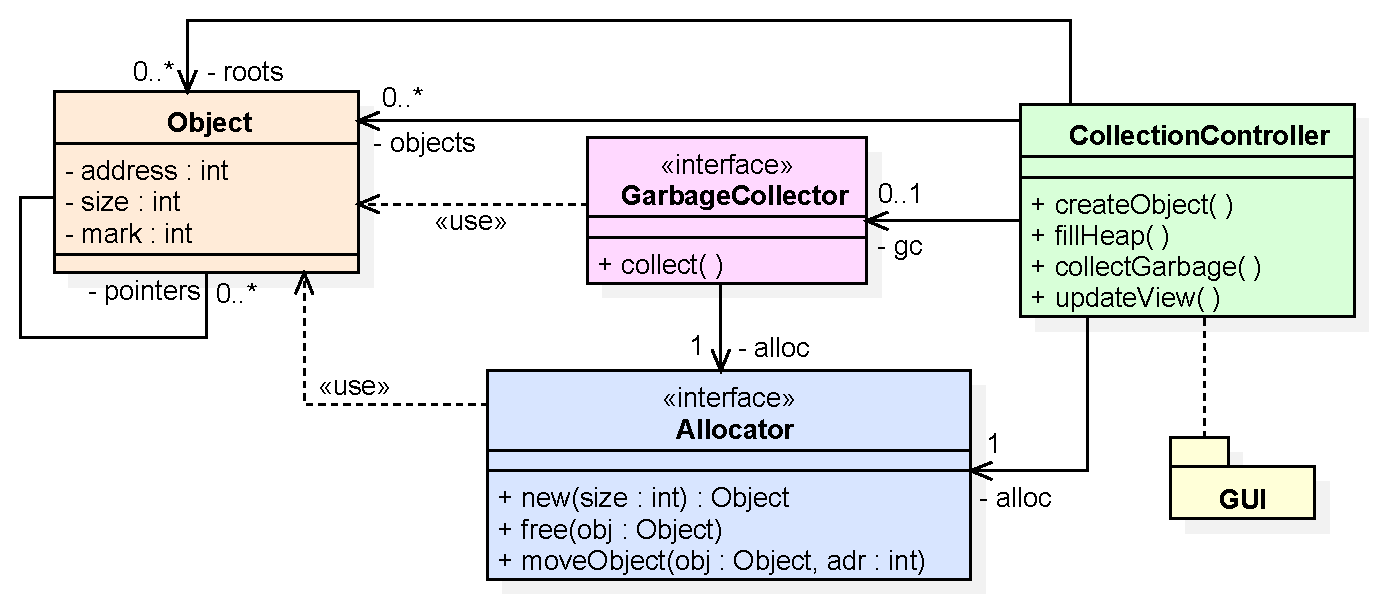
\includegraphics[scale=0.6]{img/uml/ch7-model.pdf}
	\caption[Klassendiagramm zur Modellierung von Mutator, Allokator und Kollektor]{Klassendiagramm zur Modellierung der Beziehung zwischen Mutator, Allokator und Kollektor. Im Rahmen der Implementation wurde dieses Modell um weitere Klassen, Methoden und Attribute ergänzt.}
	\label{fig:model}
\end{figure}

Heapobjekte werden als Instanzen einer Klasse \code{HeapObject} modelliert und beinhalten Speicheradresse (\code{address}), Größe (\code{size}), Markierungsinformation (\code{mark}) und eine Menge \code{pointers} an Referenzen auf weitere Instanzen von \code{HeapObject}, um die Menge \Pointers zu realisieren.
Ansonsten bieten sie keinerlei Funktionalität an.

Eine Instanz der Schnittstelle \code{Allocator} stellt die wesentlichen Dienste eines Allokators zu Verfügung.
Dazu zählt die Anforderung einer Speichermenge durch den Mutator mittels \code{new}, die Freigabe von Objekten und des durch sie belegten Speicherbereichs sowie das Verschieben eines Objekts.
Ersteres geschieht durch Übergabe der gewünschten Speichermenge und Rückgabe eines neu erzeugten Instanz von \code{HeapObject}, die die entsprechende Speicheradresse enthält.
Der Allokator ist diejenige Instanz, die Informationen über den Füllstand des Heaps und insbesondere über die Belegung einzelner Wörter besitzt.
Die Schnittstelle \code{GarbageCollector} beschreibt die Funktionalität eines Kollektors, welche im Wesentlichen aus der Durchführung eines Garbage-Collection-Zyklus (Methode \code{collect}) besteht.
Da eine Garbage Collection die Freigabe und Verschiebung von Objekten auslösen kann, verwaltet sie genau eine Instanz von \code{Allocator}.
Die Klasse \code{CollectionController} realisiert einerseits die Aufgabe des Mutators, das heißt die Anforderung von Speicher für neue Objekte sowie die (Simulation von) Referenzmanipulationen, die zur Verwaisung von Objekten führen.
Daher besitzt sie zwei Mengen von Heapobjekten \code{objects} und \code{roots}.
\code{objects} enthält dabei sämtliche Objekte des Heaps und \code{roots}\ -- entsprechend der Menge \Roots -- alle Basisobjekte.
Zudem verwaltet sie eine \code{Allocator}-Instanz, um Speicher anfordern zu können, sowie eine \code{GarbageCollector}-Instanz zur Auslösung der Garbage Collection.
Andererseits fungiert \code{CollectionController} als Steuerklasse, um über die GUI eingehende Benutzerinteraktionen umsetzen und delegieren zu können.

Die Idee ist nun, beim Start des Simulators zunächst eine Instanz der Klasse \code{CollectionController} erzeugen.
Diese legt wiederum -- je nach ausgewählter Garbage Collection -- eine geeignete \code{Allocator}-Instanz sowie einen \code{GarbageCollector} an.
Letzterer bekommt dabei den zuvor erzeugten Allokator übergeben, sodass Kollektor und Steuerklasse auf denselben simulierten Heap zugreifen.

\section{Implementation}
\label{sec:implementation}
Im nun folgenden Abschnitt wird vorgestellt, wie die obige Modellierung unter Beachtung der spezifizierten Anforderungen realisiert werden.
Im Sinne der Plattformunabhängigkeit wurde dazu die Programmiersprache \textit{Java} gewählt, wobei auf die \textit{Java Language Specification 9}\footnote{\url{https://docs.oracle.com/javase/specs/jls/se9/html/index.html}} zurückgegriffen wird.
Der gesamte Programmcode wurde über das Versionskontrollsystem \textit{Git}\footnote{\url{https://git-scm.com/}} verwaltet.
Um eine plattformunabhängige Entwicklung zu gewährleisten, wurde zudem das Build-Management-Tool \textit{Apache Maven}\footnote{\url{https://maven.apache.org/}} verwendet.
Dieses bildet die verschiedenen Arbeitsschritte der Entwicklung, wie etwa Kompilieren, Testen und Erzeugen von \code{JAR}-Dateien, auf automatisiert durchführbare Phasen ab und kümmert sich dabei eigenständig um Abhängigkeiten von externen Bibliotheken.
Zur Weiterentwicklung des Systems genügt somit ein Klonen des Git-Repositorys und eine Ausführung von Maven, um alle benötigten Abhängigkeiten beschaffen zu lassen.

Bei der Entwicklung der einzelnen Komponenten wurde grundsätzlich \textit{testgetrieben} vorgegangen.
Das bedeutet, dass zu jeder zu implementierenden Methode zunächst mehrere Testfälle erstellt werden, die das erwartete Verhalten des Programms beschreiben.
Einzige Ausnahme bilden hier Methoden, die mit GUI-Komponenten interagieren, da diese nur schwer automatisiert testbar sind.
Als Testframework wurde auf \textit{JUnit 5}\footnote{\url{https://junit.org/junit5/}} zurückgegriffen.

\newpage

\begin{figure}[H]
	\centering
	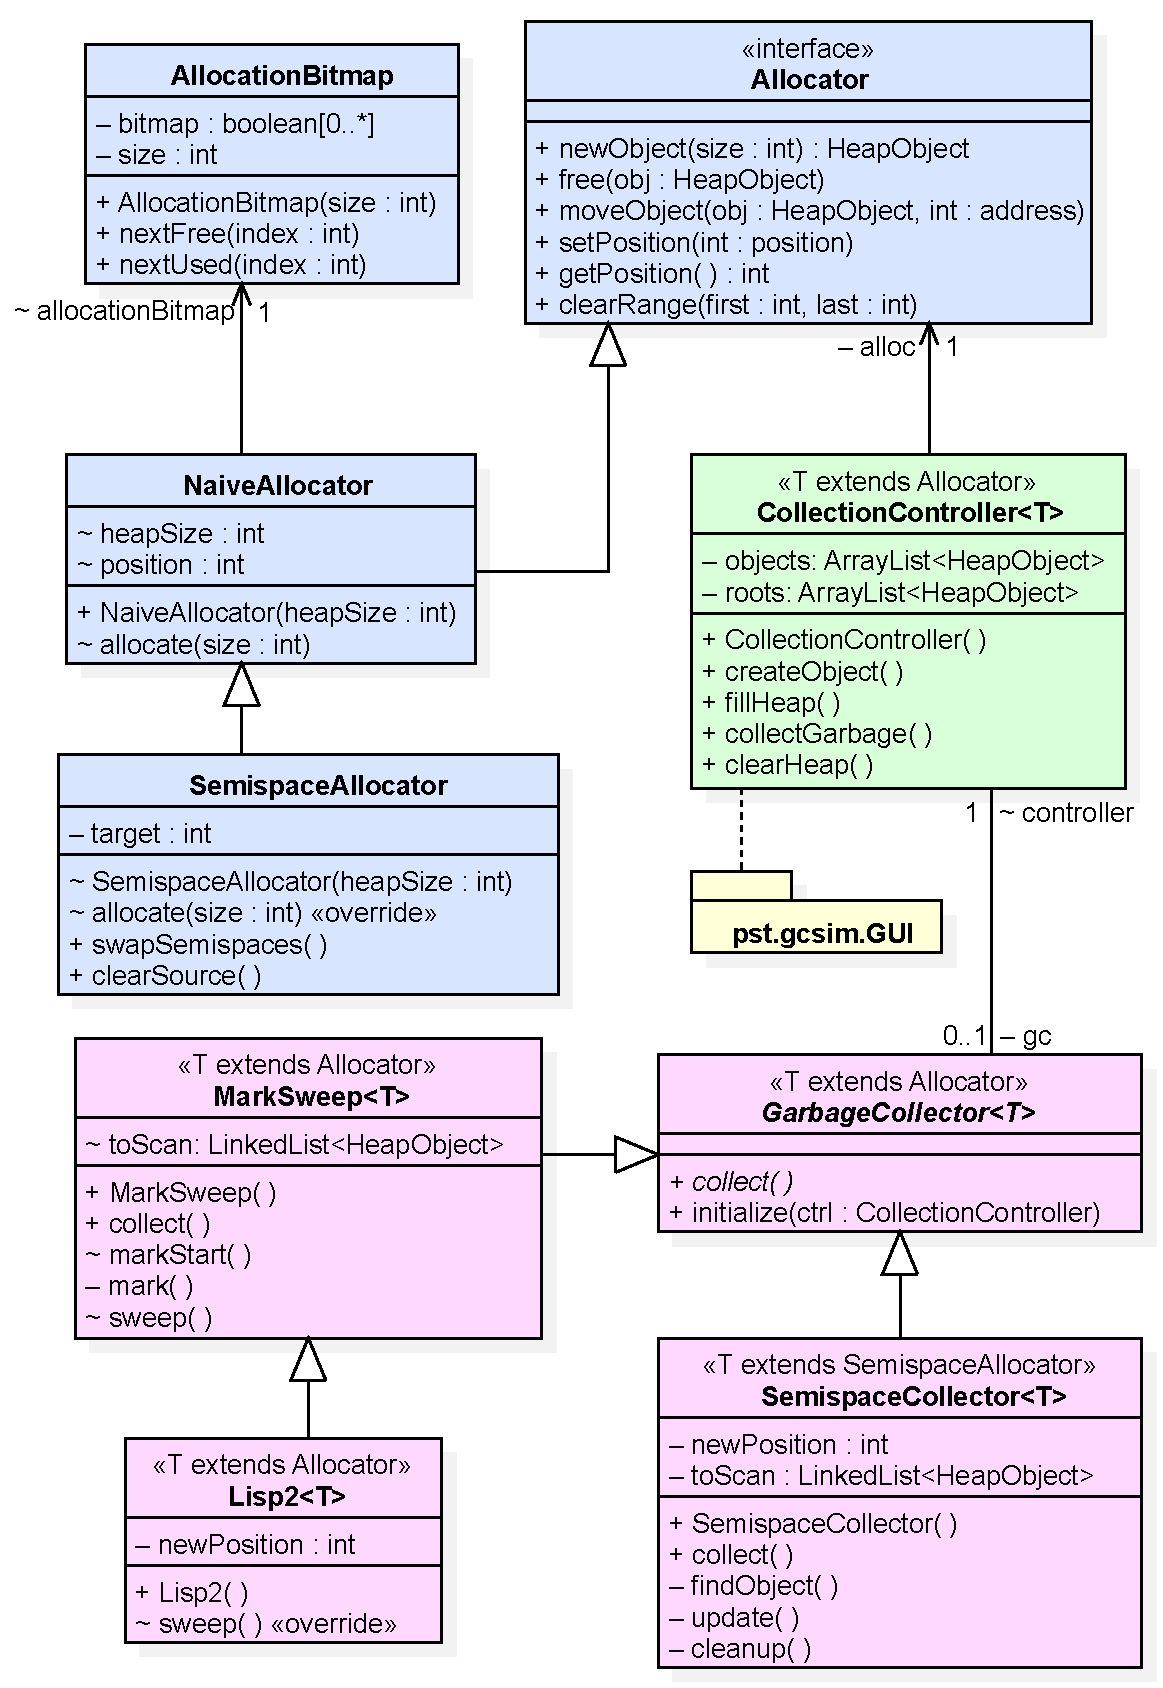
\includegraphics[scale=0.65]{img/uml/ch7-klassen.pdf}
	\caption[Klassendiagramm des realisierten Modells (Auszug)]{Klassendiagramm (Auszug) des realisierten Modells aus Abbildung~\ref{fig:model}.}
	\label{fig:implementation}
\end{figure}

\subsection{Allokator}
\label{sub:allocator}
Der Allokator verwaltet die Information, welche Wörter des simulierten Heaps belegt sind.
Aus diesem Grund wurde zunächst eine Klasse \code{AllocationBitmap} entworfen, die diese Information in einem \mintinline{java}{boolean}-Array speichert (siehe Abbildung~\ref{fig:implementation}).
Der $i$-te Eintrag dieses Arrays gibt an, ob das $i$-te Wort des Heaps durch ein Wort belegt (\mintinline{java}{true}) oder frei (\mintinline{java}{false}) ist.
Weiter stellt \code{AllocationBitmap} zwei Methoden \code{nextFree} und \code{nextUsed} zur Verfügung, welche ausgehend von einer übergebenen Speicheradresse die nächste freie bzw. belegte Stelle des Heaps liefern, indem das Array linear durchsucht wird.
Diese Methoden sind essenziell, um für eine angeforderte Speichermenge eine hinreichend große freie Stelle zu finden.

Als Konkretisierung der Schnittstelle \code{Allocator} wurde zunächst ein naiver Allokator entwickelt.
Dieser zeichnet sich dadurch aus, dass er -- ausgehend von einer Startposition -- mittels linearer Traversierung die nächstbeste freie Stelle findet, die die angeforderte Speichermenge aufnehmen kann.
Die Startposition ist dabei gegeben durch das Attribut \code{position}, welches stets die Adresse des ersten Worts hinter dem zuletzt angelegten Objekt enthält.

Das Herzstück der Klasse \code{NaiveAllocator} ist die Methode \code{allocate}, die intern durch \code{newObject} aufgerufen wird und das Auffinden einer geeigneten Position für ein neues Heapobjekt übernimmt (siehe Listing~\ref{java:naive-alloc}).
Diese Methode sucht zunächst unter Zuhilfenahme von \code{nextFree} und \code{nextUsed} der Reihe nach alle freien Stellen hinter \code{position} ab, bis eine genügend große gefunden oder das Ende des Heaps erreicht wurde (Zeile~7 bis~14).
Dabei wird auch berücksichtigt, dass sich hinter \code{position} eventuell kein freier Speicher befindet (Zeile~9f) oder ein freie Speicherbereich sich bis ans Heapende erstreckt (Zeile 12f).
Wird so ein hinreichend großer Bereich freien Speichers gefunden, wird dieser entsprechend der angeforderten Speichermenge als belegt markiert und die Anfangsadresse des Bereichs zurückgegeben (Zeile~18 bis 22).
Andernfalls wird auf analoge Weise der Bereich vor \code{position} durchsucht.
Sollte auch hierbei kein geeigneter Speicherbereich gefunden werden können, wird als Ergebnis \code{-1} zurückgegeben, was \code{newObject} dazu veranlasst, kein neues Objekt zu erzeugen.

\begin{listing}[h]
\inputminted[]{java}{code/NaiveAlloc-allocate.java}
\caption[Methode \code{allocate} der Klasse \code{NaiveAllocator}]{Auszug aus der Methode \code{allocate} der Klasse \code{NaiveAllocator}.}
\label{java:naive-alloc}
\end{listing}

Der \code{SemispaceAllocator} wurde zur Realisierung des Halbraumverfahrens nach \textsc{Fenichel}, \textsc{Yochelson} und \textsc{Cheney} (siehe Abschnitt~\ref{sec:copying}) entwickelt.
Die Allokation läuft hier weitestgehend analog zum \code{NaiveAllocator} ab, allerdings wird der Allokationsversuch auf den aktuellen Zielhalbraum beschränkt, dessen Beginn im Attribut \code{target} notiert ist.
Zusätzlich steht eine Methode \code{swapSemispaces} zur Verfügung, die die Rolle der beiden Halbräume tauscht, sowie eine Methode \code{clearSource}, die einen Halbraum in Gänze als unbelegt markiert.
\cleardoublepage

\chapter{Fazit}
Zusammenfassen, was in dieser Arbeit passiert ist.
Und, dass es noch viel mehr gibt.
Und ob der Visualisierer etwas taugt oder nicht.
%!TEX root = ../thesis.tex
\cleardoublepage
\thispagestyle{empty}

\vspace*{4.0cm}
\begin{flushright}
	\thesispartlabelfont Anhang
	{\color{ctcolorpartline}%
				\hspace*{-200pt}\rule[45pt]{600pt}{2pt}}
\end{flushright}

\setcounter{chapter}{0}
\renewcommand\thechapter{\Alph{chapter}}
\addcontentsline{toc}{part}{Anhang}

%!TEX root = ../../thesis.tex
\chapter{Beispiel zur verborgenen Referenzzählung}
\label{cha:ulterior-example}

Es sei die folgende Konstellation von Objekten in \Nursery und \Mature gegeben.
Zur Wahrung der Übersichtlichkeit sind Referenzen von \Nursery nach \Mature \textcolor{ctcolormain}{blau}, Referenzen von \Mature nach \Nursery \textcolor{ctcoloraccessory}{purpur} und Referenzen innerhalb von \Nursery \textbf{schwarz} einzgezeichnet.
Die Objekte \Var{b} und \Var{C} seien über Referenzen aus \Roots erreichbar.
In der unteren rechten Ecke eines Objekts wird der Referenzzähler angezeigt.
\Var{A} und \Var{B} seien über Referenzen innerhalb von \Mature erreichbar, besitzen also einen positiven Referenzzählerwert, der hier nicht konkret angegeben wird.
Da diese Referenzen für Algorithmus~\ref{algo:ulterior-rc} nicht relevant sind, wurden sie in der Abbildung fortgelassen.
Ebenso wurd auf die Darstellung ausgehender Referenzen bereits kopierter Objekte verzichtet.

\begin{center}
	\includestandalone[scale=1.2]{img/tikz/A-ulterior-example01}
\end{center}

Zunächst werden alle von \Roots ausgehenden Referenzen verfolgt, wobei die Objekte \Var{b} und \Var{C} entdeckt werden.
\Var{b} wird daher nach \Mature kopiert und der Referenzzähler erhöht.
Die Kopie \Var{b'} wird zu \Var{toDo} hinzugefügt, um später \Var{b} auf ausgehende Referenzen überprüfen zu können.
Da sich \Var{C} bereits in \Mature befindet, wird lediglich dessen Zähler inkrementiert.
Damit sind alle Referenzen von Basisobjekten abgearbeitet und die entsprechenden Referenzzähler von Heapobjekten angepasst.

\begin{center}
	\includestandalone[scale=1.2]{img/tikz/A-ulterior-example02}
\end{center}

Nun werden alle Referenzen von \Mature nach \Nursery verfolgt, die in \Var{log} verzeichnet sind.
Daher werden die Objekte \Var{g} und \Var{f} nach \Mature kopiert, ihre Kopien zu \Var{toDo} hinzugefügt und die Referenzzähler inkrementiert.

\begin{center}
	\includestandalone[scale=1.2]{img/tikz/A-ulterior-example03}
	
	\includestandalone[scale=1.2]{img/tikz/A-ulterior-example04}
\end{center}

Zuletzt erfolgt die Abarbeitung von \Var{toDo}.
\Var{b'} enthält eine Referenz auf das bereits kopierte Objekt \Var{f}, daher genügt es, diese Referenz anzupassen und den Referenzzähler von \Var{f'} zu erhöhen.

\begin{center}
	\includestandalone[scale=1.2]{img/tikz/A-ulterior-example05}
\end{center}

Objekt \Var{g'} besitzt eine Referenz auf \Var{c}, sodass auch dieses Objekt nach \Mature kopiert wird.

\begin{center}
	\includestandalone[scale=1.2]{img/tikz/A-ulterior-example06}
\end{center}

\Var{f'} enthält eine Referenz auf das Objekt \Var{D}, das sich bereits in \Mature befindet, sodass hier wieder ausreicht, die Referenz anzupassen und den Referenzzähler von \Var{D} zu inkrementieren.
Objekt \Var{c}, das von \Var{f'} referenziert wird, wird kopiert.

\begin{center}
	\includestandalone[scale=1.2]{img/tikz/A-ulterior-example07}
\end{center}

Die Objekte \Var{e'} und \Var{c'} weisen keine Referenzen auf andere Objekte auf, sodass mit ihrer Abarbeitung \Var{toDo} geleert wird.
Es verbleiben \Var{a} und \Var{d} in \Nursery, die nicht kopiert wurden, unerreichbar sind und somit entfernt werden.
Zugleich wird auch \Var{E} freigegeben, da sein Referenzzähler $0$ beträgt.
Nachdem die Referenzzähler von \Var{C} und \Var{b'} um die Referenzen aus \Roots korrigiert wurden, terminiert der Algorithmus.

\begin{center}
	\includestandalone[scale=1.2]{img/tikz/A-ulterior-example08}
\end{center}

%!TEX root = ../../thesis.tex
% Author: Phil Steinhorst, p.st@wwu.de

% --------------------------
% Back matter
% --------------------------
\addtocontents{toc}{\vspace{1em}}
{%
\setstretch{1.1}
\renewcommand{\bibfont}{\normalfont\small}
\setlength{\biblabelsep}{0pt}
\setlength{\bibitemsep}{0.5\baselineskip plus 0.5\baselineskip}
\printbibliography
}

\vfill

Diese Masterarbeit wurde mit \LaTeXe unter Verwendung der Vorlage \textit{Clean Thesis} von Ricardo Langner gesetzt.
Für mehr Informationen siehe \url{http://cleanthesis.der-ric.de/}.

\cleardoublepage

\chapter*{Abbildungsverzeichnis}
\addcontentsline{toc}{chapter}{Abbildungsverzeichnis}
\renewcommand\listfigurename{}
\vspace*{-2.35cm}
\listoffigures
\cleardoublepage

\chapter*{Tabellenverzeichnis}
\addcontentsline{toc}{chapter}{Tabellenverzeichnis}
\renewcommand\listtablename{}
\vspace*{-2.35cm}
\listoftables
\cleardoublepage

% !TEX root = ../../thesis.tex
% Author: Phil Steinhorst, p.st@wwu.de
\addcontentsline{toc}{chapter}{Eigenständigkeitserklärung}
\chapter*{Eigenständigkeitserklärung}
\label{sec:declaration}
Hiermit versichere ich, dass die vorliegende Masterarbeit mit dem Titel \textit{\thesisTitle} selbstständig verfasst worden ist, dass keine anderen Quellen und Hilfsmittel als die angegebenen benutzt worden sind und dass die Stellen der Arbeit, die anderen Werken -- auch elektronischen Medien -- dem Wortlaut oder Sinn nach entnommen wurden, auf jeden Fall unter Angabe der Quelle als Entlehnung kenntlich gemacht worden sind.

Ich erkläre mich mit einem Abgleich der Arbeit mit anderen Texten zwecks Auffindung von Übereinstimmungen sowie mit einer zu diesem Zweck vorzunehmenden Speicherung der Arbeit in eine Datenbank einverstanden.

\vspace*{2cm}

\begin{minipage}{0.5\textwidth}
	\begin{flushleft} \large
		\underline{\hspace{6cm}} \\
		{\footnotesize (Ort, Datum)}
	\end{flushleft}
\end{minipage}
~
\begin{minipage}{0.5\textwidth}
	\begin{flushright} \large
		\underline{\hspace{6cm}} \\
		{\footnotesize (Unterschrift)}
	\end{flushright}
\end{minipage}\\[0.5cm]
%\clearpage
%\newpage
%\mbox{}
\end{document}
